% Options for packages loaded elsewhere
\PassOptionsToPackage{unicode}{hyperref}
\PassOptionsToPackage{hyphens}{url}
%
\documentclass[
]{article}
\usepackage{amsmath,amssymb}
\usepackage{lmodern}
\usepackage{iftex}
\ifPDFTeX
  \usepackage[T1]{fontenc}
  \usepackage[utf8]{inputenc}
  \usepackage{textcomp} % provide euro and other symbols
\else % if luatex or xetex
  \usepackage{unicode-math}
  \defaultfontfeatures{Scale=MatchLowercase}
  \defaultfontfeatures[\rmfamily]{Ligatures=TeX,Scale=1}
\fi
% Use upquote if available, for straight quotes in verbatim environments
\IfFileExists{upquote.sty}{\usepackage{upquote}}{}
\IfFileExists{microtype.sty}{% use microtype if available
  \usepackage[]{microtype}
  \UseMicrotypeSet[protrusion]{basicmath} % disable protrusion for tt fonts
}{}
\makeatletter
\@ifundefined{KOMAClassName}{% if non-KOMA class
  \IfFileExists{parskip.sty}{%
    \usepackage{parskip}
  }{% else
    \setlength{\parindent}{0pt}
    \setlength{\parskip}{6pt plus 2pt minus 1pt}}
}{% if KOMA class
  \KOMAoptions{parskip=half}}
\makeatother
\usepackage{xcolor}
\usepackage[margin=1in]{geometry}
\usepackage{graphicx}
\makeatletter
\def\maxwidth{\ifdim\Gin@nat@width>\linewidth\linewidth\else\Gin@nat@width\fi}
\def\maxheight{\ifdim\Gin@nat@height>\textheight\textheight\else\Gin@nat@height\fi}
\makeatother
% Scale images if necessary, so that they will not overflow the page
% margins by default, and it is still possible to overwrite the defaults
% using explicit options in \includegraphics[width, height, ...]{}
\setkeys{Gin}{width=\maxwidth,height=\maxheight,keepaspectratio}
% Set default figure placement to htbp
\makeatletter
\def\fps@figure{htbp}
\makeatother
\setlength{\emergencystretch}{3em} % prevent overfull lines
\providecommand{\tightlist}{%
  \setlength{\itemsep}{0pt}\setlength{\parskip}{0pt}}
\setcounter{secnumdepth}{-\maxdimen} % remove section numbering
\usepackage{multirow}
\usepackage{multicol}
\usepackage{colortbl}
\usepackage{hhline}
\usepackage{longtable}
\usepackage{float}
\usepackage{wrapfig}
\usepackage{array}
\usepackage{hyperref}
\ifLuaTeX
  \usepackage{selnolig}  % disable illegal ligatures
\fi
\IfFileExists{bookmark.sty}{\usepackage{bookmark}}{\usepackage{hyperref}}
\IfFileExists{xurl.sty}{\usepackage{xurl}}{} % add URL line breaks if available
\urlstyle{same} % disable monospaced font for URLs
\hypersetup{
  pdftitle={WIP: Suffolk Annual Waste Monitoring Report 21/22},
  hidelinks,
  pdfcreator={LaTeX via pandoc}}

\title{WIP: Suffolk Annual Waste Monitoring Report 21/22}
\author{}
\date{\vspace{-2.5em}}

\begin{document}
\maketitle

\newpage

\hypertarget{introduction}{%
\section{Introduction}\label{introduction}}

The Suffolk Minerals \& Waste Local Plan was adopted in July 2020. The
Plan contains a Vision explaining how the County will meet its statutory
obligation for the supply of aggregates and the sustainable management
of waste.

It contains policies for determining planning application for minerals
and waste development and identifies sites for future development for
these uses.

It is important to understand whether the policies in the Plan are being
delivered as intended and the extent to which the waste arisings and
movements that were forecast are correct. Because of the nature of waste
data, such forecasts will never be exact, but trends can be identified
and broad conclusions reached.

The Plan identifies sites that are suitable for the management of waste
and this Monitoring Report will examine whether such sites have been
taken forward for this use, or whether the policies should be amended in
a future Plan.

The Local Plan contains a Policy Monitoring Framework which identifies
the Performance Indicators that will be used to monitor the Plan which
are the number of times that the relevant policies are triggered in the
decision-making process.

Suffolk County Council also has a Development Management Local
Monitoring and Enforcement Plan, adopted in 2016. This sets out how the
Council deals with the monitoring of developments as they are delivered
including site visits to ensure that planning conditions are being
carried out as intended.

This report looks at the effectiveness of the waste policies in
delivering the policy outcomes in the Plan. In particular it examines
whether Suffolk is net self-sufficient in the management of the waste
arising with the Plan Area or whether additional waste management
facilities are required to achieve this.

\hypertarget{coronavirus-covid-19-the-impact-of-the-pandemic-on-local-authority-waste-collection-and-services}{%
\subsection{Coronavirus (COVID-19): The impact of the pandemic on local
authority waste collection and
services}\label{coronavirus-covid-19-the-impact-of-the-pandemic-on-local-authority-waste-collection-and-services}}

When reading this report, and especially when comparing annual totals
between 2020/21 and 2021/22, the context of the pandemic should be taken
into account.

The COVID-19 pandemic, which commenced in March 2020, caused disruption
to local authority waste collection services. Services were heavily
disrupted during April to June 2020.

As restrictions eased through the summer and into the autumn of 2020,
local authorities and businesses acclimatised to working under lockdown
conditions, and there was less disruption to services in the remainder
of 2020. During 2021 lockdown restrictions were eased and despite
further waves of infection there was less disruption to waste services.

Wider issues, such as the state of the economy during the pandemic will
also have had an effect on the amount of waste generated.

A
\href{https://www.instituteforgovernment.org.uk/sites/default/files/2022-12/timeline-coronavirus-lockdown-december-2021.pdf}{full
timeline of the UK government coronavirus lockdown} is available. A more
in-depth analysis of the impact of the COVID-19 pandemic on waste
services is given in the
\href{https://www.gov.uk/government/statistics/local-authority-collected-waste-management-annual-results-202122/local-authority-collected-waste-management-annual-results-202122\#coronavirus-covid-19-the-impact-of-the-pandemic-on-local-authority-waste-collection-and-services}{Local
authority collected waste management - annual results 2021/22 report}
from the Department for Environment Food \& Rural Affairs (DEFRA).

\newpage

\hypertarget{methodology}{%
\section{Methodology}\label{methodology}}

\hypertarget{data-sources}{%
\subsection{Data Sources}\label{data-sources}}

\begin{itemize}
\tightlist
\item
  The Local Authority Collected Waste annual results found under
  \href{https://www.gov.uk/government/statistical-data-sets/env18-local-authority-collected-waste-annual-results-tables-202122}{ENV18
  - Local Authority Collected Waste}, produced by DEFRA, for Section 3.
  These annual results are published alongside a
  \href{https://www.gov.uk/government/statistics/local-authority-collected-waste-management-annual-results-202122/local-authority-collected-waste-management-annual-results-202122\#coronavirus-covid-19-the-impact-of-the-pandemic-on-local-authority-waste-collection-and-services}{national
  statistical report}.
\item
  The
  \href{https://www.data.gov.uk/dataset/0e0c12d8-24f6-461f-b4bc-f6d6a5bf2de5/wastedataflow-local-authority-waste-management}{WasteDataFlow
  - Local Authority waste management} dataset, covering collection and
  recycling of waste based on a quarterly survey from local authorities,
  for section 3.3.
\item
  The
  \href{https://find-data-beta.cloudapps.digital/dataset/d409b2ba-796c-4436-82c7-eb1831a9ef25/2019-waste-data-interrogator}{Waste
  Data Interrogator 2019},
  \href{https://www.data.gov.uk/dataset/bb40d091-a346-4b75-aa54-df7d347bed93/2020-waste-data-interrogator}{2020}
  and
  \href{https://www.data.gov.uk/dataset/d8a12b93-03ef-4fbf-9a43-1ca7a054479c/2021-waste-data-interrogator}{2021},
  produced by the Environment Agency, for Sections 4 and 5.
\item
  The
  \href{https://www.data.gov.uk/dataset/237825cb-dc10-4c53-8446-1bcd35614c12/remaining-landfill-capacity}{Remaining
  Landfill Capacity 2019-2021} dataset produced by the Environment
  Agency for Section 4.3.
\end{itemize}

\hypertarget{code}{%
\subsection{Code}\label{code}}

This report was generated in R Markdown. The source code for this
report, all figures and calculations are provided in a
\href{https://github.com/SCC-Planning/wamreport}{Github repository}.
Full documentation is provided, and will allow other local authorities
in England to generate their own annual waste monitoring report by
adapting the code.

\newpage

\hypertarget{waste-managed-in-suffolk}{%
\section{Waste Managed in Suffolk}\label{waste-managed-in-suffolk}}

\hypertarget{local-authority-collected-waste}{%
\subsection{Local Authority Collected
Waste}\label{local-authority-collected-waste}}

The total amount of Local Authority Collected Waste (LACW) in Suffolk,
after a reduction dip in 2020-21, has increased again to a similar level
as before the pandemic as shown in Figure @ref(fig:totallocalauthority):

\begin{figure}
\centering
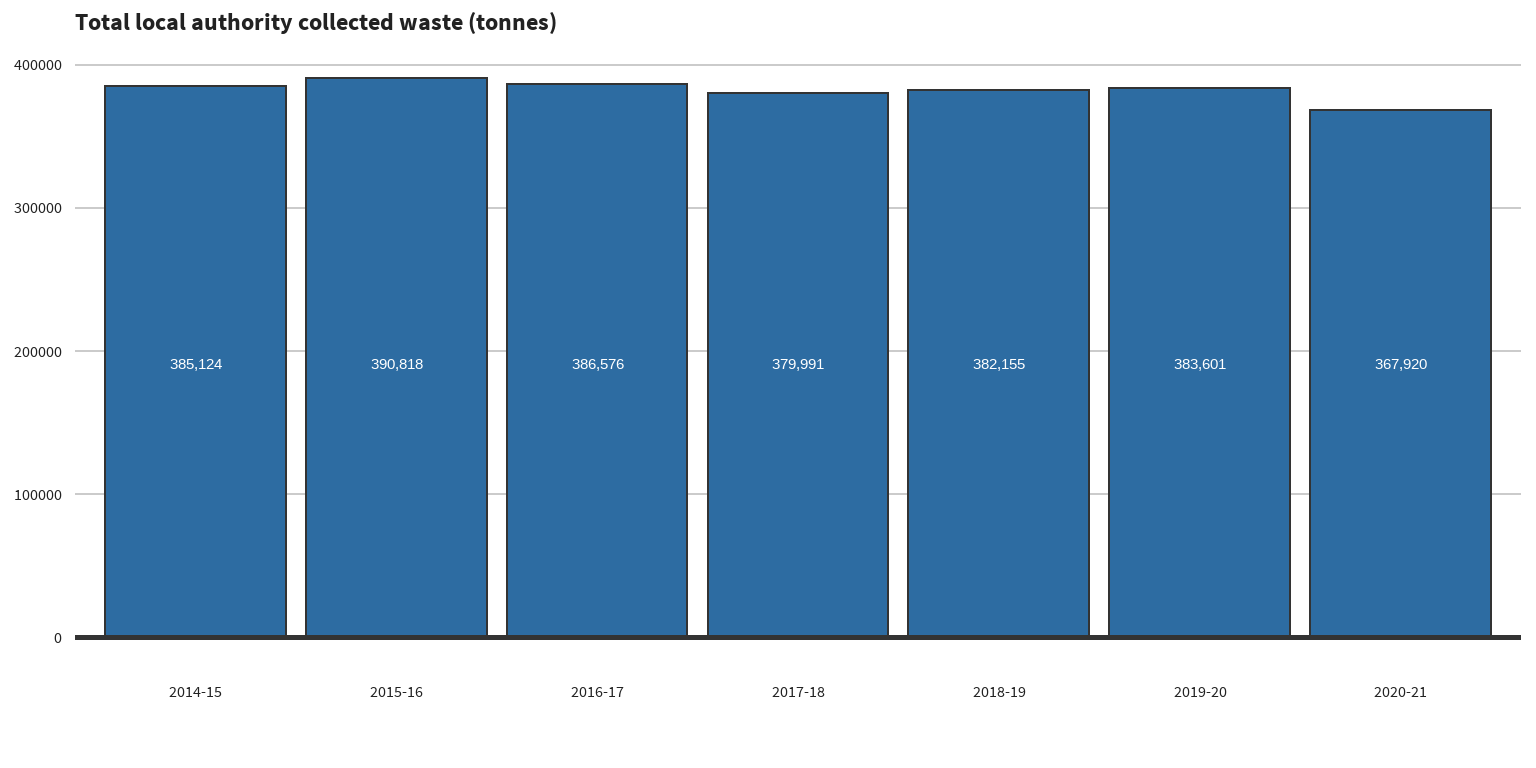
\includegraphics{index_files/figure-latex/totallocalauthority-1.pdf}
\caption{\label{fig:totallocalauthority}Source:
\href{https://www.gov.uk/government/statistical-data-sets/env18-local-authority-collected-waste-annual-results-tables}{ENV18
- Local Authority Collected Waste}}
\end{figure}

Household waste arising has also returned to a level similar to that
before 2020-21, as shown in Figure @ref(fig:householdwaste).

This is in line of expectation, and similar to the national picture,
which saw household waste increase with the easing of lockdown in Spring
2021.

Consumption overall may have reduced as a result of lower economic
activity in 2020-21, and returned to previous levels as economic
activity has ramped up again in 2021-22.

\begin{figure}
\centering
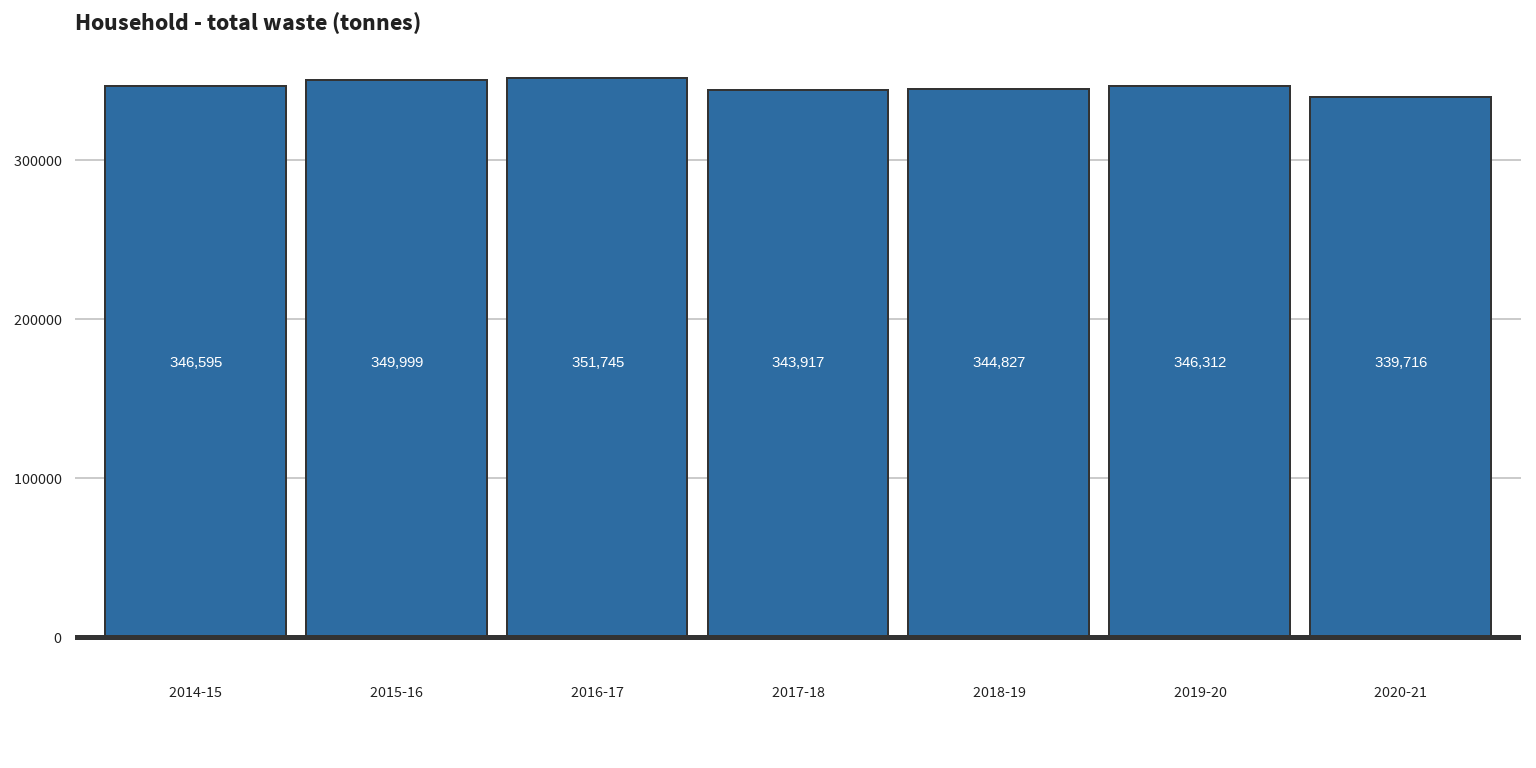
\includegraphics{index_files/figure-latex/householdwaste-1.pdf}
\caption{Source:
\href{https://www.gov.uk/government/statistical-data-sets/env18-local-authority-collected-waste-annual-results-tables}{ENV18
- Local Authority Collected Waste}}
\end{figure}

\hypertarget{waste-sent-to-recycling-and-recycling-rates}{%
\subsection{Waste sent to Recycling and Recycling
Rates}\label{waste-sent-to-recycling-and-recycling-rates}}

The amount of LACW sent for recycling has steadily reduced between
2015-16 and 2020-21, as shown in Figure @ref(fig:sentforrecycling). In
2021-22 however, there is again an increase in the amount of household
waste set for recycling/composting/reuse. It should be noted however
that it is still a smaller when compared to 2019-20, pre-pandemic.

\begin{figure}
\centering
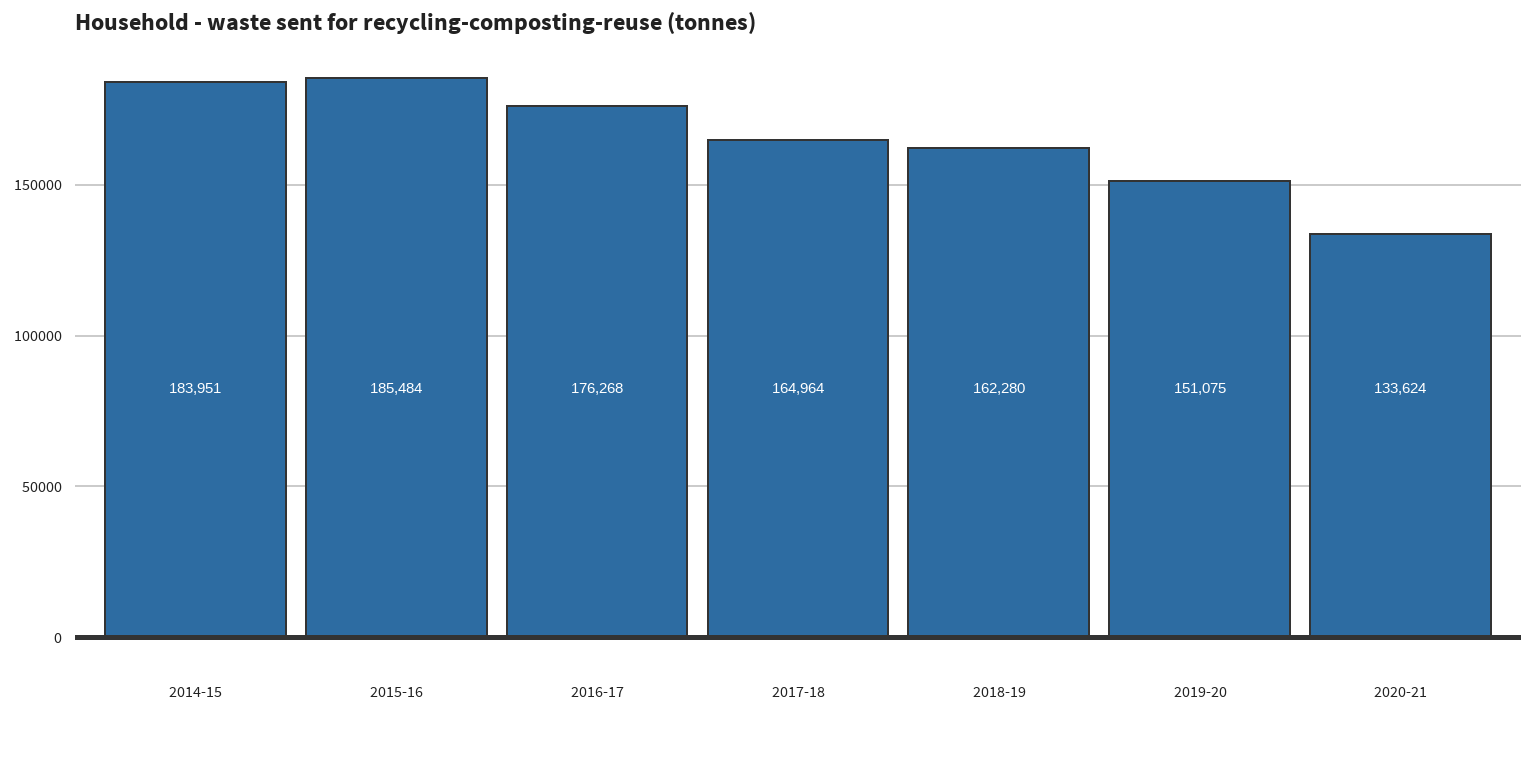
\includegraphics{index_files/figure-latex/sentforrecycling-1.pdf}
\caption{Source:
\href{https://www.gov.uk/government/statistical-data-sets/env18-local-authority-collected-waste-annual-results-tables}{ENV18
- Local Authority Collected Waste}}
\end{figure}

Suffolk historically had one of the highest recycling rates in England
but this has reduced in all the Suffolk Districts over the past seven
years as shown in Table @ref(tab:recyclingrates). It should be noted
that the recycling rate in Suffolk is now lower than the official
recycling rate in England as a whole (44.1\%).

Compared to last year, the recycling rate as a percentage has stayed
constant. This indicates that, although in absolute tonnage more
household waste has been sent for recycling/composting/reuse in 2021-22,
as shown in Table @ref(fig:sentforrecycling), this is a result the total
local authority collected waste increasing and not due to an increase in
the recycling rates.

\providecommand{\docline}[3]{\noalign{\global\setlength{\arrayrulewidth}{#1}}\arrayrulecolor[HTML]{#2}\cline{#3}}

\setlength{\tabcolsep}{0pt}

\renewcommand*{\arraystretch}{1.5}

\begin{longtable}[c]{cc}

\caption{\textcolor[HTML]{000000}{\fontsize{11}{13}\selectfont{Source:\ [ENV18\ -\ Local\ Authority\ Collected\ Waste](https://www.gov.uk/government/statistical-data-sets/env18-local-authority-collected-waste-annual-results-tables)}}}\\

\hhline{>{\arrayrulecolor[HTML]{666666}\global\arrayrulewidth=2pt}->{\arrayrulecolor[HTML]{666666}\global\arrayrulewidth=2pt}-}

\multicolumn{1}{!{\color[HTML]{000000}\vrule width 0pt}>{}l}{\textcolor[HTML]{000000}{\fontsize{11}{11}\selectfont{\textbf{Financial\ Year}}}} & \multicolumn{1}{!{\color[HTML]{000000}\vrule width 0pt}>{}r!{\color[HTML]{000000}\vrule width 0pt}}{\textcolor[HTML]{000000}{\fontsize{11}{11}\selectfont{\textbf{\%\ sent\ for\ recycling}}}} \\

\hhline{>{\arrayrulecolor[HTML]{666666}\global\arrayrulewidth=2pt}->{\arrayrulecolor[HTML]{666666}\global\arrayrulewidth=2pt}-}\endhead



\multicolumn{1}{!{\color[HTML]{000000}\vrule width 0pt}>{}l}{\textcolor[HTML]{000000}{\fontsize{11}{11}\selectfont{2014-15}}} & \multicolumn{1}{!{\color[HTML]{000000}\vrule width 0pt}>{}r!{\color[HTML]{000000}\vrule width 0pt}}{\textcolor[HTML]{000000}{\fontsize{11}{11}\selectfont{51.7}}} \\

\hhline{>{\arrayrulecolor[HTML]{666666}\global\arrayrulewidth=0.5pt}->{\arrayrulecolor[HTML]{666666}\global\arrayrulewidth=0.5pt}-}



\multicolumn{1}{!{\color[HTML]{000000}\vrule width 0pt}>{}l}{\textcolor[HTML]{000000}{\fontsize{11}{11}\selectfont{2015-16}}} & \multicolumn{1}{!{\color[HTML]{000000}\vrule width 0pt}>{}r!{\color[HTML]{000000}\vrule width 0pt}}{\textcolor[HTML]{000000}{\fontsize{11}{11}\selectfont{51.7}}} \\

\hhline{>{\arrayrulecolor[HTML]{666666}\global\arrayrulewidth=0.5pt}->{\arrayrulecolor[HTML]{666666}\global\arrayrulewidth=0.5pt}-}



\multicolumn{1}{!{\color[HTML]{000000}\vrule width 0pt}>{}l}{\textcolor[HTML]{000000}{\fontsize{11}{11}\selectfont{2016-17}}} & \multicolumn{1}{!{\color[HTML]{000000}\vrule width 0pt}>{}r!{\color[HTML]{000000}\vrule width 0pt}}{\textcolor[HTML]{000000}{\fontsize{11}{11}\selectfont{48.1}}} \\

\hhline{>{\arrayrulecolor[HTML]{666666}\global\arrayrulewidth=0.5pt}->{\arrayrulecolor[HTML]{666666}\global\arrayrulewidth=0.5pt}-}



\multicolumn{1}{!{\color[HTML]{000000}\vrule width 0pt}>{}l}{\textcolor[HTML]{000000}{\fontsize{11}{11}\selectfont{2017-18}}} & \multicolumn{1}{!{\color[HTML]{000000}\vrule width 0pt}>{}r!{\color[HTML]{000000}\vrule width 0pt}}{\textcolor[HTML]{000000}{\fontsize{11}{11}\selectfont{46.1}}} \\

\hhline{>{\arrayrulecolor[HTML]{666666}\global\arrayrulewidth=0.5pt}->{\arrayrulecolor[HTML]{666666}\global\arrayrulewidth=0.5pt}-}



\multicolumn{1}{!{\color[HTML]{000000}\vrule width 0pt}>{}l}{\textcolor[HTML]{000000}{\fontsize{11}{11}\selectfont{2018-19}}} & \multicolumn{1}{!{\color[HTML]{000000}\vrule width 0pt}>{}r!{\color[HTML]{000000}\vrule width 0pt}}{\textcolor[HTML]{000000}{\fontsize{11}{11}\selectfont{45.3}}} \\

\hhline{>{\arrayrulecolor[HTML]{666666}\global\arrayrulewidth=0.5pt}->{\arrayrulecolor[HTML]{666666}\global\arrayrulewidth=0.5pt}-}



\multicolumn{1}{!{\color[HTML]{000000}\vrule width 0pt}>{}l}{\textcolor[HTML]{000000}{\fontsize{11}{11}\selectfont{2019-20}}} & \multicolumn{1}{!{\color[HTML]{000000}\vrule width 0pt}>{}r!{\color[HTML]{000000}\vrule width 0pt}}{\textcolor[HTML]{000000}{\fontsize{11}{11}\selectfont{42.1}}} \\

\hhline{>{\arrayrulecolor[HTML]{666666}\global\arrayrulewidth=0.5pt}->{\arrayrulecolor[HTML]{666666}\global\arrayrulewidth=0.5pt}-}



\multicolumn{1}{!{\color[HTML]{000000}\vrule width 0pt}>{}l}{\textcolor[HTML]{000000}{\fontsize{11}{11}\selectfont{2020-21}}} & \multicolumn{1}{!{\color[HTML]{000000}\vrule width 0pt}>{}r!{\color[HTML]{000000}\vrule width 0pt}}{\textcolor[HTML]{000000}{\fontsize{11}{11}\selectfont{38.3}}} \\

\hhline{>{\arrayrulecolor[HTML]{666666}\global\arrayrulewidth=0.5pt}->{\arrayrulecolor[HTML]{666666}\global\arrayrulewidth=0.5pt}-}



\multicolumn{1}{!{\color[HTML]{000000}\vrule width 0pt}>{}l}{\textcolor[HTML]{000000}{\fontsize{11}{11}\selectfont{2021-22}}} & \multicolumn{1}{!{\color[HTML]{000000}\vrule width 0pt}>{}r!{\color[HTML]{000000}\vrule width 0pt}}{\textcolor[HTML]{000000}{\fontsize{11}{11}\selectfont{38.3}}} \\

\hhline{>{\arrayrulecolor[HTML]{666666}\global\arrayrulewidth=2pt}->{\arrayrulecolor[HTML]{666666}\global\arrayrulewidth=2pt}-}



\end{longtable}

The LACW recycling rate is shown in Figure
@ref(fig:districtrecyclingratedistricts) for each of the Suffolk
Districts. These have been subject to some reorganisaition in recent
years and so the graphs below show the rates for the combines councils
before each merger and the current district. It is possible that the
process of re-organisation has disrupted services to some extent.

From 2019 - 20, Suffolk Coastal District Council and Waveney District
Council merged to become East Suffolk Council, and Forest Heath District
Council and St Edmundsbury Borough Council merged to become West Suffolk
Council. Their figures have been aggregated in their respective
Councils.

\begin{figure}
\centering
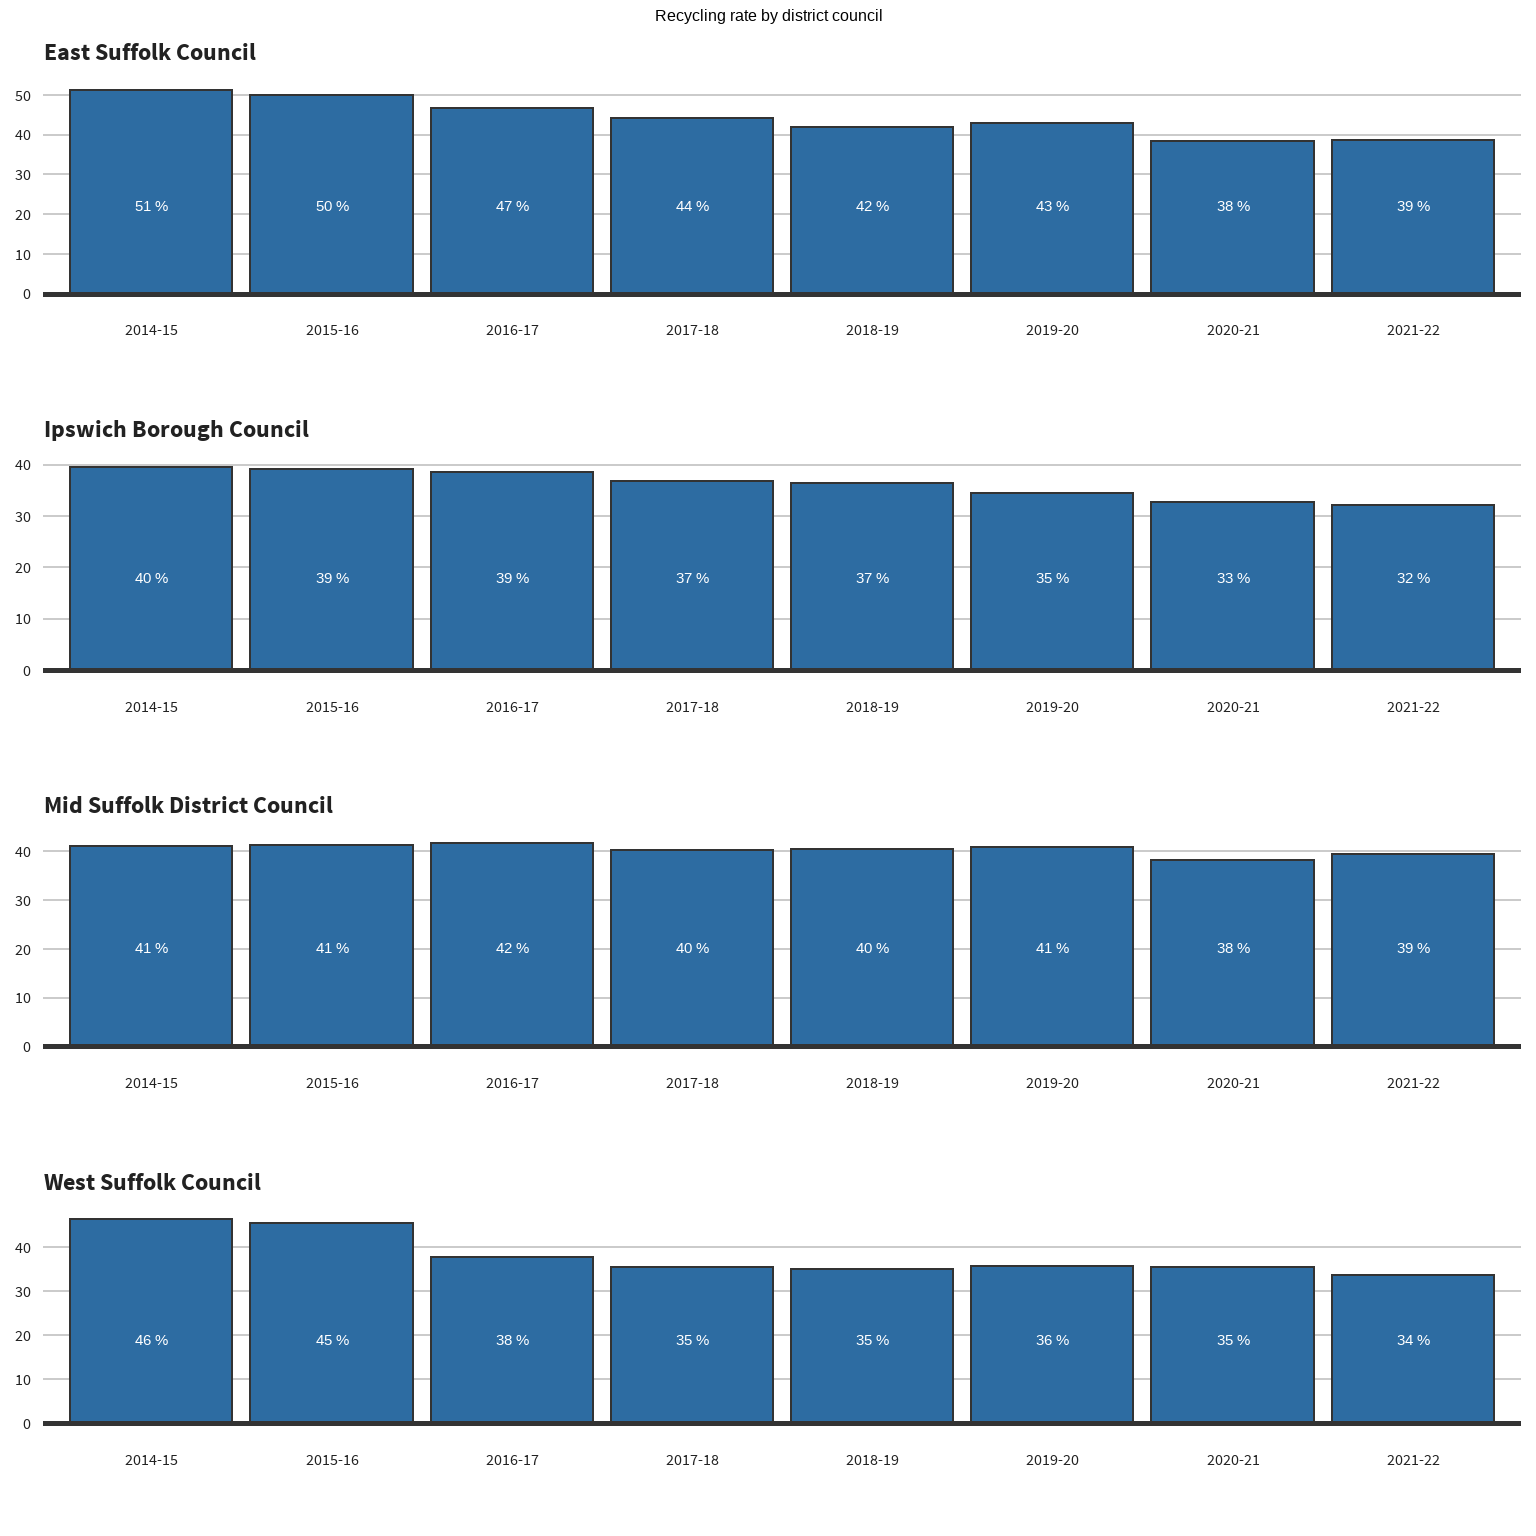
\includegraphics{index_files/figure-latex/districtrecyclingratedistricts-1.pdf}
\caption{Source:
\href{https://www.gov.uk/government/statistical-data-sets/env18-local-authority-collected-waste-annual-results-tables}{ENV18
- Local Authority Collected Waste}}
\end{figure}

\hypertarget{case-study-food-waste-collection}{%
\subsection{Case Study: Food Waste
Collection}\label{case-study-food-waste-collection}}

Currently no food waste is collected separately in Suffolk. However, as
part of the Environment Act 2021 authorities will be expected to collect
food waste separately at least once a week. Authorities which do not
have an existing food waste collection contract in place, will be
expected to make arrangements by the 2024/25 financial year at the
latest.

Although food waste is not collected in Suffolk, there are 119
authorities in England that already collect food waste separately. To
try and estimate how much food waste we might expect to arise, we can
look at how much food waste is collected as a percentage of the total
waste collected by these authorities.

To get an impression of the performance of neighbouring authorities,
Table @ref(tab:foodwastenearby) provides a summary of some of the
neighbouring authorities that already collect food waste separately, and
their food waste collection rates.

\providecommand{\docline}[3]{\noalign{\global\setlength{\arrayrulewidth}{#1}}\arrayrulecolor[HTML]{#2}\cline{#3}}

\setlength{\tabcolsep}{0pt}

\renewcommand*{\arraystretch}{1.5}

\begin{longtable}[c]{cccc}

\caption{\textcolor[HTML]{000000}{\fontsize{11}{13}\selectfont{Source:\ [WasteDataFlow\ -\ Local\ Authority\ waste\ management](https://www.data.gov.uk/dataset/0e0c12d8-24f6-461f-b4bc-f6d6a5bf2de5/wastedataflow-local-authority-waste-management)}}}\\

\hhline{>{\arrayrulecolor[HTML]{666666}\global\arrayrulewidth=2pt}->{\arrayrulecolor[HTML]{666666}\global\arrayrulewidth=2pt}->{\arrayrulecolor[HTML]{666666}\global\arrayrulewidth=2pt}->{\arrayrulecolor[HTML]{666666}\global\arrayrulewidth=2pt}-}

\multicolumn{4}{!{\color[HTML]{000000}\vrule width 0pt}>{}l!{\color[HTML]{000000}\vrule width 0pt}}{\textcolor[HTML]{000000}{\fontsize{11}{11}\selectfont{\textbf{Food\ Waste\ Collection\ Rates\ in\ selected\ authorities\ near\ Suffolk,\ 2021-22}}}} \\

\hhline{>{\arrayrulecolor[HTML]{666666}\global\arrayrulewidth=0.5pt}->{\arrayrulecolor[HTML]{666666}\global\arrayrulewidth=0.5pt}->{\arrayrulecolor[HTML]{666666}\global\arrayrulewidth=0.5pt}->{\arrayrulecolor[HTML]{666666}\global\arrayrulewidth=0.5pt}-}



\multicolumn{1}{!{\color[HTML]{000000}\vrule width 0pt}>{}l}{\textcolor[HTML]{000000}{\fontsize{11}{11}\selectfont{\textbf{Authority}}}} & \multicolumn{1}{!{\color[HTML]{000000}\vrule width 0pt}>{}r}{\textcolor[HTML]{000000}{\fontsize{11}{11}\selectfont{\textbf{Food\ Waste\ Collected\ (in\ t)}}}} & \multicolumn{1}{!{\color[HTML]{000000}\vrule width 0pt}>{}r}{\textcolor[HTML]{000000}{\fontsize{11}{11}\selectfont{\textbf{Total\ Household\ Waste\ Collected\ (in\ t)}}}} & \multicolumn{1}{!{\color[HTML]{000000}\vrule width 0pt}>{}r!{\color[HTML]{000000}\vrule width 0pt}}{\textcolor[HTML]{000000}{\fontsize{11}{11}\selectfont{\textbf{\%\ Food\ Waste\ of\ Total\ Collected}}}} \\

\hhline{>{\arrayrulecolor[HTML]{666666}\global\arrayrulewidth=2pt}->{\arrayrulecolor[HTML]{666666}\global\arrayrulewidth=2pt}->{\arrayrulecolor[HTML]{666666}\global\arrayrulewidth=2pt}->{\arrayrulecolor[HTML]{666666}\global\arrayrulewidth=2pt}-}\endhead



\multicolumn{1}{!{\color[HTML]{000000}\vrule width 0pt}>{}l}{\textcolor[HTML]{000000}{\fontsize{11}{11}\selectfont{Cambridge\ City\ and\ South\ Cambs\ Councils}}} & \multicolumn{1}{!{\color[HTML]{000000}\vrule width 0pt}>{}r}{\textcolor[HTML]{000000}{\fontsize{11}{11}\selectfont{1,042.84}}} & \multicolumn{1}{!{\color[HTML]{000000}\vrule width 0pt}>{}r}{\textcolor[HTML]{000000}{\fontsize{11}{11}\selectfont{107,230}}} & \multicolumn{1}{!{\color[HTML]{000000}\vrule width 0pt}>{}r!{\color[HTML]{000000}\vrule width 0pt}}{\textcolor[HTML]{000000}{\fontsize{11}{11}\selectfont{0.97\%}}} \\

\hhline{>{\arrayrulecolor[HTML]{666666}\global\arrayrulewidth=0.5pt}->{\arrayrulecolor[HTML]{666666}\global\arrayrulewidth=0.5pt}->{\arrayrulecolor[HTML]{666666}\global\arrayrulewidth=0.5pt}->{\arrayrulecolor[HTML]{666666}\global\arrayrulewidth=0.5pt}-}



\multicolumn{1}{!{\color[HTML]{000000}\vrule width 0pt}>{}l}{\textcolor[HTML]{000000}{\fontsize{11}{11}\selectfont{Colchester\ Borough\ Council}}} & \multicolumn{1}{!{\color[HTML]{000000}\vrule width 0pt}>{}r}{\textcolor[HTML]{000000}{\fontsize{11}{11}\selectfont{6,509.92}}} & \multicolumn{1}{!{\color[HTML]{000000}\vrule width 0pt}>{}r}{\textcolor[HTML]{000000}{\fontsize{11}{11}\selectfont{64,333}}} & \multicolumn{1}{!{\color[HTML]{000000}\vrule width 0pt}>{}r!{\color[HTML]{000000}\vrule width 0pt}}{\textcolor[HTML]{000000}{\fontsize{11}{11}\selectfont{10.12\%}}} \\

\hhline{>{\arrayrulecolor[HTML]{666666}\global\arrayrulewidth=0.5pt}->{\arrayrulecolor[HTML]{666666}\global\arrayrulewidth=0.5pt}->{\arrayrulecolor[HTML]{666666}\global\arrayrulewidth=0.5pt}->{\arrayrulecolor[HTML]{666666}\global\arrayrulewidth=0.5pt}-}



\multicolumn{1}{!{\color[HTML]{000000}\vrule width 0pt}>{}l}{\textcolor[HTML]{000000}{\fontsize{11}{11}\selectfont{Kings\ Lynn\ and\ West\ Norfolk\ Borough\ Council}}} & \multicolumn{1}{!{\color[HTML]{000000}\vrule width 0pt}>{}r}{\textcolor[HTML]{000000}{\fontsize{11}{11}\selectfont{1,178.06}}} & \multicolumn{1}{!{\color[HTML]{000000}\vrule width 0pt}>{}r}{\textcolor[HTML]{000000}{\fontsize{11}{11}\selectfont{64,404}}} & \multicolumn{1}{!{\color[HTML]{000000}\vrule width 0pt}>{}r!{\color[HTML]{000000}\vrule width 0pt}}{\textcolor[HTML]{000000}{\fontsize{11}{11}\selectfont{1.83\%}}} \\

\hhline{>{\arrayrulecolor[HTML]{666666}\global\arrayrulewidth=0.5pt}->{\arrayrulecolor[HTML]{666666}\global\arrayrulewidth=0.5pt}->{\arrayrulecolor[HTML]{666666}\global\arrayrulewidth=0.5pt}->{\arrayrulecolor[HTML]{666666}\global\arrayrulewidth=0.5pt}-}



\multicolumn{1}{!{\color[HTML]{000000}\vrule width 0pt}>{}l}{\textcolor[HTML]{000000}{\fontsize{11}{11}\selectfont{Maldon\ District\ Council}}} & \multicolumn{1}{!{\color[HTML]{000000}\vrule width 0pt}>{}r}{\textcolor[HTML]{000000}{\fontsize{11}{11}\selectfont{2,440.14}}} & \multicolumn{1}{!{\color[HTML]{000000}\vrule width 0pt}>{}r}{\textcolor[HTML]{000000}{\fontsize{11}{11}\selectfont{25,859}}} & \multicolumn{1}{!{\color[HTML]{000000}\vrule width 0pt}>{}r!{\color[HTML]{000000}\vrule width 0pt}}{\textcolor[HTML]{000000}{\fontsize{11}{11}\selectfont{9.44\%}}} \\

\hhline{>{\arrayrulecolor[HTML]{666666}\global\arrayrulewidth=0.5pt}->{\arrayrulecolor[HTML]{666666}\global\arrayrulewidth=0.5pt}->{\arrayrulecolor[HTML]{666666}\global\arrayrulewidth=0.5pt}->{\arrayrulecolor[HTML]{666666}\global\arrayrulewidth=0.5pt}-}



\multicolumn{1}{!{\color[HTML]{000000}\vrule width 0pt}>{}l}{\textcolor[HTML]{000000}{\fontsize{11}{11}\selectfont{Norwich\ City\ Council}}} & \multicolumn{1}{!{\color[HTML]{000000}\vrule width 0pt}>{}r}{\textcolor[HTML]{000000}{\fontsize{11}{11}\selectfont{3,405.96}}} & \multicolumn{1}{!{\color[HTML]{000000}\vrule width 0pt}>{}r}{\textcolor[HTML]{000000}{\fontsize{11}{11}\selectfont{47,121}}} & \multicolumn{1}{!{\color[HTML]{000000}\vrule width 0pt}>{}r!{\color[HTML]{000000}\vrule width 0pt}}{\textcolor[HTML]{000000}{\fontsize{11}{11}\selectfont{7.23\%}}} \\

\hhline{>{\arrayrulecolor[HTML]{666666}\global\arrayrulewidth=0.5pt}->{\arrayrulecolor[HTML]{666666}\global\arrayrulewidth=0.5pt}->{\arrayrulecolor[HTML]{666666}\global\arrayrulewidth=0.5pt}->{\arrayrulecolor[HTML]{666666}\global\arrayrulewidth=0.5pt}-}



\multicolumn{1}{!{\color[HTML]{000000}\vrule width 0pt}>{}l}{\textcolor[HTML]{000000}{\fontsize{11}{11}\selectfont{Peterborough\ City\ Council}}} & \multicolumn{1}{!{\color[HTML]{000000}\vrule width 0pt}>{}r}{\textcolor[HTML]{000000}{\fontsize{11}{11}\selectfont{5,404.20}}} & \multicolumn{1}{!{\color[HTML]{000000}\vrule width 0pt}>{}r}{\textcolor[HTML]{000000}{\fontsize{11}{11}\selectfont{86,036}}} & \multicolumn{1}{!{\color[HTML]{000000}\vrule width 0pt}>{}r!{\color[HTML]{000000}\vrule width 0pt}}{\textcolor[HTML]{000000}{\fontsize{11}{11}\selectfont{6.28\%}}} \\

\hhline{>{\arrayrulecolor[HTML]{666666}\global\arrayrulewidth=0.5pt}->{\arrayrulecolor[HTML]{666666}\global\arrayrulewidth=0.5pt}->{\arrayrulecolor[HTML]{666666}\global\arrayrulewidth=0.5pt}->{\arrayrulecolor[HTML]{666666}\global\arrayrulewidth=0.5pt}-}



\multicolumn{1}{!{\color[HTML]{000000}\vrule width 0pt}>{}l}{\textcolor[HTML]{000000}{\fontsize{11}{11}\selectfont{Tendring\ District\ Council}}} & \multicolumn{1}{!{\color[HTML]{000000}\vrule width 0pt}>{}r}{\textcolor[HTML]{000000}{\fontsize{11}{11}\selectfont{4,318.76}}} & \multicolumn{1}{!{\color[HTML]{000000}\vrule width 0pt}>{}r}{\textcolor[HTML]{000000}{\fontsize{11}{11}\selectfont{52,857}}} & \multicolumn{1}{!{\color[HTML]{000000}\vrule width 0pt}>{}r!{\color[HTML]{000000}\vrule width 0pt}}{\textcolor[HTML]{000000}{\fontsize{11}{11}\selectfont{8.17\%}}} \\

\hhline{>{\arrayrulecolor[HTML]{666666}\global\arrayrulewidth=2pt}->{\arrayrulecolor[HTML]{666666}\global\arrayrulewidth=2pt}->{\arrayrulecolor[HTML]{666666}\global\arrayrulewidth=2pt}->{\arrayrulecolor[HTML]{666666}\global\arrayrulewidth=2pt}-}



\end{longtable}

The national picture is showin in summary statistics, which are provided
here in Table @ref(tab:foodwastesummary).

\providecommand{\docline}[3]{\noalign{\global\setlength{\arrayrulewidth}{#1}}\arrayrulecolor[HTML]{#2}\cline{#3}}

\setlength{\tabcolsep}{0pt}

\renewcommand*{\arraystretch}{1.5}

\begin{longtable}[c]{cc}

\caption{\textcolor[HTML]{000000}{\fontsize{11}{13}\selectfont{Source:\ [WasteDataFlow\ -\ Local\ Authority\ waste\ management](https://www.data.gov.uk/dataset/0e0c12d8-24f6-461f-b4bc-f6d6a5bf2de5/wastedataflow-local-authority-waste-management)}}}\\

\hhline{>{\arrayrulecolor[HTML]{666666}\global\arrayrulewidth=2pt}->{\arrayrulecolor[HTML]{666666}\global\arrayrulewidth=2pt}-}

\multicolumn{2}{!{\color[HTML]{000000}\vrule width 0pt}>{}l!{\color[HTML]{000000}\vrule width 0pt}}{\textcolor[HTML]{000000}{\fontsize{11}{11}\selectfont{\textbf{Statistics\ for\ Food\ Waste\ as\ a\ percentage\ of\ total\ household\ waste\ collected,\ England\ 2021-22}}}} \\

\hhline{>{\arrayrulecolor[HTML]{666666}\global\arrayrulewidth=0.5pt}->{\arrayrulecolor[HTML]{666666}\global\arrayrulewidth=0.5pt}-}



\multicolumn{1}{!{\color[HTML]{000000}\vrule width 0pt}>{}l}{\textcolor[HTML]{000000}{\fontsize{11}{11}\selectfont{\textbf{Summary\ Statistic}}}} & \multicolumn{1}{!{\color[HTML]{000000}\vrule width 0pt}>{}r!{\color[HTML]{000000}\vrule width 0pt}}{\textcolor[HTML]{000000}{\fontsize{11}{11}\selectfont{\textbf{Food\ waste\ collection\ rate}}}} \\

\hhline{>{\arrayrulecolor[HTML]{666666}\global\arrayrulewidth=2pt}->{\arrayrulecolor[HTML]{666666}\global\arrayrulewidth=2pt}-}\endhead



\multicolumn{1}{!{\color[HTML]{000000}\vrule width 0pt}>{}l}{\textcolor[HTML]{000000}{\fontsize{11}{11}\selectfont{Min.}}} & \multicolumn{1}{!{\color[HTML]{000000}\vrule width 0pt}>{}r!{\color[HTML]{000000}\vrule width 0pt}}{\textcolor[HTML]{000000}{\fontsize{11}{11}\selectfont{0.06\%}}} \\

\hhline{>{\arrayrulecolor[HTML]{666666}\global\arrayrulewidth=0.5pt}->{\arrayrulecolor[HTML]{666666}\global\arrayrulewidth=0.5pt}-}



\multicolumn{1}{!{\color[HTML]{000000}\vrule width 0pt}>{}l}{\textcolor[HTML]{000000}{\fontsize{11}{11}\selectfont{1st\ Qu.}}} & \multicolumn{1}{!{\color[HTML]{000000}\vrule width 0pt}>{}r!{\color[HTML]{000000}\vrule width 0pt}}{\textcolor[HTML]{000000}{\fontsize{11}{11}\selectfont{4.44\%}}} \\

\hhline{>{\arrayrulecolor[HTML]{666666}\global\arrayrulewidth=0.5pt}->{\arrayrulecolor[HTML]{666666}\global\arrayrulewidth=0.5pt}-}



\multicolumn{1}{!{\color[HTML]{000000}\vrule width 0pt}>{}l}{\textcolor[HTML]{000000}{\fontsize{11}{11}\selectfont{Median}}} & \multicolumn{1}{!{\color[HTML]{000000}\vrule width 0pt}>{}r!{\color[HTML]{000000}\vrule width 0pt}}{\textcolor[HTML]{000000}{\fontsize{11}{11}\selectfont{7.30\%}}} \\

\hhline{>{\arrayrulecolor[HTML]{666666}\global\arrayrulewidth=0.5pt}->{\arrayrulecolor[HTML]{666666}\global\arrayrulewidth=0.5pt}-}



\multicolumn{1}{!{\color[HTML]{000000}\vrule width 0pt}>{}l}{\textcolor[HTML]{000000}{\fontsize{11}{11}\selectfont{Mean}}} & \multicolumn{1}{!{\color[HTML]{000000}\vrule width 0pt}>{}r!{\color[HTML]{000000}\vrule width 0pt}}{\textcolor[HTML]{000000}{\fontsize{11}{11}\selectfont{6.71\%}}} \\

\hhline{>{\arrayrulecolor[HTML]{666666}\global\arrayrulewidth=0.5pt}->{\arrayrulecolor[HTML]{666666}\global\arrayrulewidth=0.5pt}-}



\multicolumn{1}{!{\color[HTML]{000000}\vrule width 0pt}>{}l}{\textcolor[HTML]{000000}{\fontsize{11}{11}\selectfont{3rd\ Qu.}}} & \multicolumn{1}{!{\color[HTML]{000000}\vrule width 0pt}>{}r!{\color[HTML]{000000}\vrule width 0pt}}{\textcolor[HTML]{000000}{\fontsize{11}{11}\selectfont{8.97\%}}} \\

\hhline{>{\arrayrulecolor[HTML]{666666}\global\arrayrulewidth=0.5pt}->{\arrayrulecolor[HTML]{666666}\global\arrayrulewidth=0.5pt}-}



\multicolumn{1}{!{\color[HTML]{000000}\vrule width 0pt}>{}l}{\textcolor[HTML]{000000}{\fontsize{11}{11}\selectfont{Max.}}} & \multicolumn{1}{!{\color[HTML]{000000}\vrule width 0pt}>{}r!{\color[HTML]{000000}\vrule width 0pt}}{\textcolor[HTML]{000000}{\fontsize{11}{11}\selectfont{15.40\%}}} \\

\hhline{>{\arrayrulecolor[HTML]{666666}\global\arrayrulewidth=2pt}->{\arrayrulecolor[HTML]{666666}\global\arrayrulewidth=2pt}-}



\end{longtable}

The mean recycling rate of food waste across all authorities that
collect it is \textbf{6.71\%}, with a minimum rate of \textbf{0.06\%}
and a maximum rate of \textbf{15.4\%}. The 1st quartile and 3rd quartile
indicate that, in simple terms, the rate for most authorities lies
between \textbf{4.44 - 8.97 \%}.

An exact number cannot be predicted. Therefore, using the summary
statistics in Table @ref(tab:foodwastesummary), we can estimate a likely
range of food waste tonnage that might arise when food waste is
collected separately.

By multiplying the total household waste collected in each of the
districts, by the national food waste collection rates above, an
estimated range is given in Figure @ref(fig:foodwastepredicted).

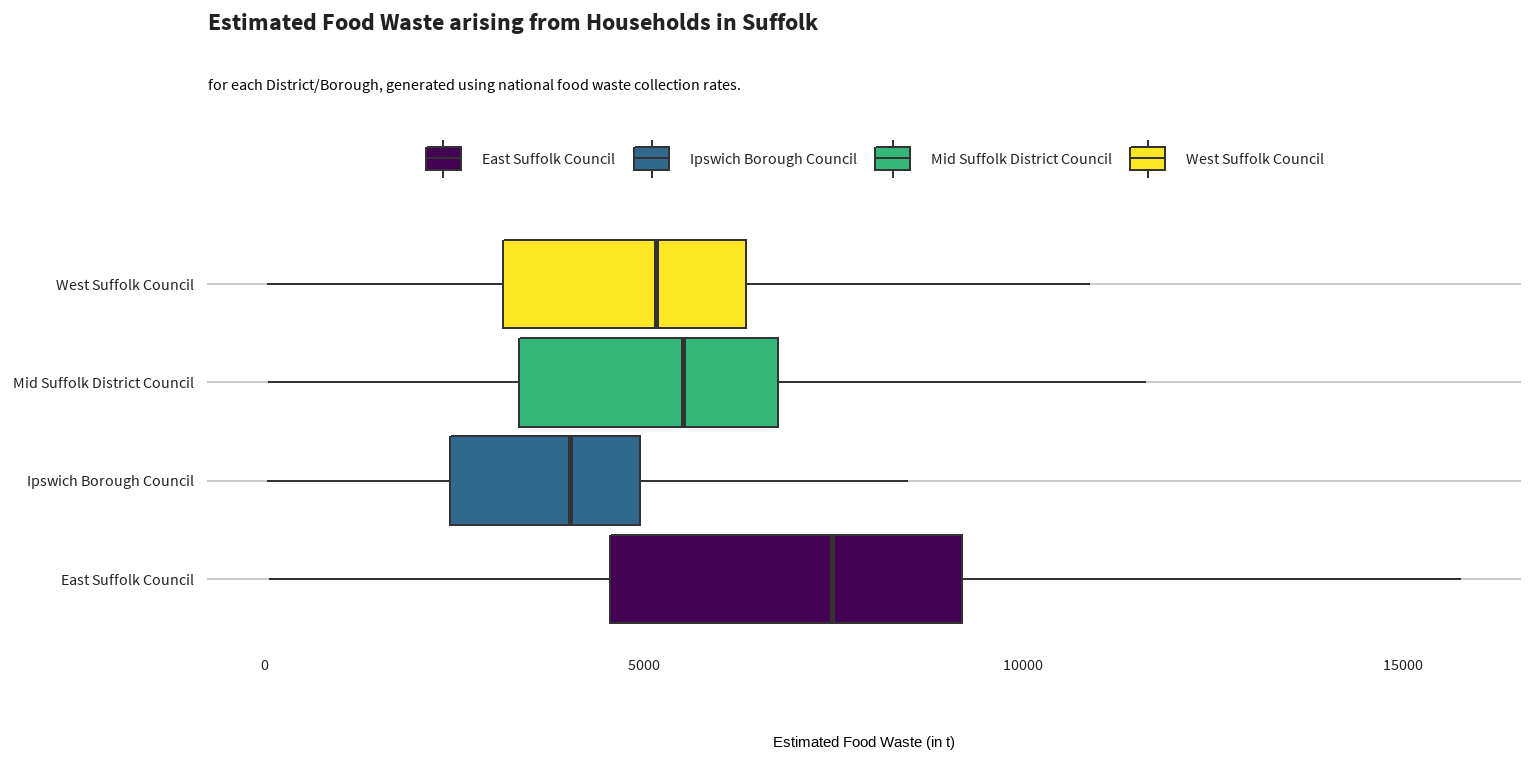
\includegraphics{index_files/figure-latex/foodwastepredicted-1.pdf} The
totals displayed in Figure @ref(fig:foodwastepredicted) are stated in
Table @ref(tab:foodwasteestimate). This shows the estimated tonnage of
food waste, where the lowest estimate is equivalent to the lowest food
waste collection rate in England, low is equivalent to the 1st quartile
in the England etc.

\providecommand{\docline}[3]{\noalign{\global\setlength{\arrayrulewidth}{#1}}\arrayrulecolor[HTML]{#2}\cline{#3}}

\setlength{\tabcolsep}{0pt}

\renewcommand*{\arraystretch}{1.5}

\begin{longtable}[c]{cccccc}

\caption{\textcolor[HTML]{000000}{\fontsize{11}{13}\selectfont{Source:\ [WasteDataFlow\ -\ Local\ Authority\ waste\ management](https://www.data.gov.uk/dataset/0e0c12d8-24f6-461f-b4bc-f6d6a5bf2de5/wastedataflow-local-authority-waste-management)}}}\\

\hhline{>{\arrayrulecolor[HTML]{666666}\global\arrayrulewidth=2pt}->{\arrayrulecolor[HTML]{666666}\global\arrayrulewidth=2pt}->{\arrayrulecolor[HTML]{666666}\global\arrayrulewidth=2pt}->{\arrayrulecolor[HTML]{666666}\global\arrayrulewidth=2pt}->{\arrayrulecolor[HTML]{666666}\global\arrayrulewidth=2pt}->{\arrayrulecolor[HTML]{666666}\global\arrayrulewidth=2pt}-}

\multicolumn{6}{!{\color[HTML]{000000}\vrule width 0pt}>{}l!{\color[HTML]{000000}\vrule width 0pt}}{\textcolor[HTML]{000000}{\fontsize{11}{11}\selectfont{\textbf{Estimated\ Food\ Waste\ arising\ from\ Households\ in\ Suffolk,\ England\ 2021-22\ (tonnes)}}}} \\

\hhline{>{\arrayrulecolor[HTML]{666666}\global\arrayrulewidth=0.5pt}->{\arrayrulecolor[HTML]{666666}\global\arrayrulewidth=0.5pt}->{\arrayrulecolor[HTML]{666666}\global\arrayrulewidth=0.5pt}->{\arrayrulecolor[HTML]{666666}\global\arrayrulewidth=0.5pt}->{\arrayrulecolor[HTML]{666666}\global\arrayrulewidth=0.5pt}->{\arrayrulecolor[HTML]{666666}\global\arrayrulewidth=0.5pt}-}



\multicolumn{1}{!{\color[HTML]{000000}\vrule width 0pt}>{}l}{\textcolor[HTML]{000000}{\fontsize{11}{11}\selectfont{\textbf{Authority}}}} & \multicolumn{1}{!{\color[HTML]{000000}\vrule width 0pt}>{}r}{\textcolor[HTML]{000000}{\fontsize{11}{11}\selectfont{\textbf{Lowest\ Estimate}}}} & \multicolumn{1}{!{\color[HTML]{000000}\vrule width 0pt}>{}r}{\textcolor[HTML]{000000}{\fontsize{11}{11}\selectfont{\textbf{Low\ Estimate}}}} & \multicolumn{1}{!{\color[HTML]{000000}\vrule width 0pt}>{}r}{\textcolor[HTML]{000000}{\fontsize{11}{11}\selectfont{\textbf{Median\ Estimate}}}} & \multicolumn{1}{!{\color[HTML]{000000}\vrule width 0pt}>{}r}{\textcolor[HTML]{000000}{\fontsize{11}{11}\selectfont{\textbf{High\ Estimate}}}} & \multicolumn{1}{!{\color[HTML]{000000}\vrule width 0pt}>{}r!{\color[HTML]{000000}\vrule width 0pt}}{\textcolor[HTML]{000000}{\fontsize{11}{11}\selectfont{\textbf{Highest\ Estimate}}}} \\

\hhline{>{\arrayrulecolor[HTML]{666666}\global\arrayrulewidth=2pt}->{\arrayrulecolor[HTML]{666666}\global\arrayrulewidth=2pt}->{\arrayrulecolor[HTML]{666666}\global\arrayrulewidth=2pt}->{\arrayrulecolor[HTML]{666666}\global\arrayrulewidth=2pt}->{\arrayrulecolor[HTML]{666666}\global\arrayrulewidth=2pt}->{\arrayrulecolor[HTML]{666666}\global\arrayrulewidth=2pt}-}\endhead



\multicolumn{1}{!{\color[HTML]{000000}\vrule width 0pt}>{}l}{\textcolor[HTML]{000000}{\fontsize{11}{11}\selectfont{East\ Suffolk\ Council}}} & \multicolumn{1}{!{\color[HTML]{000000}\vrule width 0pt}>{}r}{\textcolor[HTML]{000000}{\fontsize{11}{11}\selectfont{61}}} & \multicolumn{1}{!{\color[HTML]{000000}\vrule width 0pt}>{}r}{\textcolor[HTML]{000000}{\fontsize{11}{11}\selectfont{4,548}}} & \multicolumn{1}{!{\color[HTML]{000000}\vrule width 0pt}>{}r}{\textcolor[HTML]{000000}{\fontsize{11}{11}\selectfont{7,478}}} & \multicolumn{1}{!{\color[HTML]{000000}\vrule width 0pt}>{}r}{\textcolor[HTML]{000000}{\fontsize{11}{11}\selectfont{9,187}}} & \multicolumn{1}{!{\color[HTML]{000000}\vrule width 0pt}>{}r!{\color[HTML]{000000}\vrule width 0pt}}{\textcolor[HTML]{000000}{\fontsize{11}{11}\selectfont{15,766}}} \\

\hhline{>{\arrayrulecolor[HTML]{666666}\global\arrayrulewidth=0.5pt}->{\arrayrulecolor[HTML]{666666}\global\arrayrulewidth=0.5pt}->{\arrayrulecolor[HTML]{666666}\global\arrayrulewidth=0.5pt}->{\arrayrulecolor[HTML]{666666}\global\arrayrulewidth=0.5pt}->{\arrayrulecolor[HTML]{666666}\global\arrayrulewidth=0.5pt}->{\arrayrulecolor[HTML]{666666}\global\arrayrulewidth=0.5pt}-}



\multicolumn{1}{!{\color[HTML]{000000}\vrule width 0pt}>{}l}{\textcolor[HTML]{000000}{\fontsize{11}{11}\selectfont{Ipswich\ Borough\ Council}}} & \multicolumn{1}{!{\color[HTML]{000000}\vrule width 0pt}>{}r}{\textcolor[HTML]{000000}{\fontsize{11}{11}\selectfont{33}}} & \multicolumn{1}{!{\color[HTML]{000000}\vrule width 0pt}>{}r}{\textcolor[HTML]{000000}{\fontsize{11}{11}\selectfont{2,448}}} & \multicolumn{1}{!{\color[HTML]{000000}\vrule width 0pt}>{}r}{\textcolor[HTML]{000000}{\fontsize{11}{11}\selectfont{4,024}}} & \multicolumn{1}{!{\color[HTML]{000000}\vrule width 0pt}>{}r}{\textcolor[HTML]{000000}{\fontsize{11}{11}\selectfont{4,944}}} & \multicolumn{1}{!{\color[HTML]{000000}\vrule width 0pt}>{}r!{\color[HTML]{000000}\vrule width 0pt}}{\textcolor[HTML]{000000}{\fontsize{11}{11}\selectfont{8,484}}} \\

\hhline{>{\arrayrulecolor[HTML]{666666}\global\arrayrulewidth=0.5pt}->{\arrayrulecolor[HTML]{666666}\global\arrayrulewidth=0.5pt}->{\arrayrulecolor[HTML]{666666}\global\arrayrulewidth=0.5pt}->{\arrayrulecolor[HTML]{666666}\global\arrayrulewidth=0.5pt}->{\arrayrulecolor[HTML]{666666}\global\arrayrulewidth=0.5pt}->{\arrayrulecolor[HTML]{666666}\global\arrayrulewidth=0.5pt}-}



\multicolumn{1}{!{\color[HTML]{000000}\vrule width 0pt}>{}l}{\textcolor[HTML]{000000}{\fontsize{11}{11}\selectfont{Mid\ Suffolk\ District\ Council}}} & \multicolumn{1}{!{\color[HTML]{000000}\vrule width 0pt}>{}r}{\textcolor[HTML]{000000}{\fontsize{11}{11}\selectfont{45}}} & \multicolumn{1}{!{\color[HTML]{000000}\vrule width 0pt}>{}r}{\textcolor[HTML]{000000}{\fontsize{11}{11}\selectfont{3,351}}} & \multicolumn{1}{!{\color[HTML]{000000}\vrule width 0pt}>{}r}{\textcolor[HTML]{000000}{\fontsize{11}{11}\selectfont{5,510}}} & \multicolumn{1}{!{\color[HTML]{000000}\vrule width 0pt}>{}r}{\textcolor[HTML]{000000}{\fontsize{11}{11}\selectfont{6,769}}} & \multicolumn{1}{!{\color[HTML]{000000}\vrule width 0pt}>{}r!{\color[HTML]{000000}\vrule width 0pt}}{\textcolor[HTML]{000000}{\fontsize{11}{11}\selectfont{11,616}}} \\

\hhline{>{\arrayrulecolor[HTML]{666666}\global\arrayrulewidth=0.5pt}->{\arrayrulecolor[HTML]{666666}\global\arrayrulewidth=0.5pt}->{\arrayrulecolor[HTML]{666666}\global\arrayrulewidth=0.5pt}->{\arrayrulecolor[HTML]{666666}\global\arrayrulewidth=0.5pt}->{\arrayrulecolor[HTML]{666666}\global\arrayrulewidth=0.5pt}->{\arrayrulecolor[HTML]{666666}\global\arrayrulewidth=0.5pt}-}



\multicolumn{1}{!{\color[HTML]{000000}\vrule width 0pt}>{}l}{\textcolor[HTML]{000000}{\fontsize{11}{11}\selectfont{West\ Suffolk\ Council}}} & \multicolumn{1}{!{\color[HTML]{000000}\vrule width 0pt}>{}r}{\textcolor[HTML]{000000}{\fontsize{11}{11}\selectfont{42}}} & \multicolumn{1}{!{\color[HTML]{000000}\vrule width 0pt}>{}r}{\textcolor[HTML]{000000}{\fontsize{11}{11}\selectfont{3,138}}} & \multicolumn{1}{!{\color[HTML]{000000}\vrule width 0pt}>{}r}{\textcolor[HTML]{000000}{\fontsize{11}{11}\selectfont{5,160}}} & \multicolumn{1}{!{\color[HTML]{000000}\vrule width 0pt}>{}r}{\textcolor[HTML]{000000}{\fontsize{11}{11}\selectfont{6,339}}} & \multicolumn{1}{!{\color[HTML]{000000}\vrule width 0pt}>{}r!{\color[HTML]{000000}\vrule width 0pt}}{\textcolor[HTML]{000000}{\fontsize{11}{11}\selectfont{10,879}}} \\

\hhline{>{\arrayrulecolor[HTML]{666666}\global\arrayrulewidth=0.5pt}->{\arrayrulecolor[HTML]{666666}\global\arrayrulewidth=0.5pt}->{\arrayrulecolor[HTML]{666666}\global\arrayrulewidth=0.5pt}->{\arrayrulecolor[HTML]{666666}\global\arrayrulewidth=0.5pt}->{\arrayrulecolor[HTML]{666666}\global\arrayrulewidth=0.5pt}->{\arrayrulecolor[HTML]{666666}\global\arrayrulewidth=0.5pt}-}



\multicolumn{1}{!{\color[HTML]{000000}\vrule width 0pt}>{}l}{\textcolor[HTML]{000000}{\fontsize{11}{11}\selectfont{\textbf{Suffolk\ Total}}}} & \multicolumn{1}{!{\color[HTML]{000000}\vrule width 0pt}>{}r}{\textcolor[HTML]{000000}{\fontsize{11}{11}\selectfont{\textbf{180}}}} & \multicolumn{1}{!{\color[HTML]{000000}\vrule width 0pt}>{}r}{\textcolor[HTML]{000000}{\fontsize{11}{11}\selectfont{\textbf{13,485}}}} & \multicolumn{1}{!{\color[HTML]{000000}\vrule width 0pt}>{}r}{\textcolor[HTML]{000000}{\fontsize{11}{11}\selectfont{\textbf{22,172}}}} & \multicolumn{1}{!{\color[HTML]{000000}\vrule width 0pt}>{}r}{\textcolor[HTML]{000000}{\fontsize{11}{11}\selectfont{\textbf{27,238}}}} & \multicolumn{1}{!{\color[HTML]{000000}\vrule width 0pt}>{}r!{\color[HTML]{000000}\vrule width 0pt}}{\textcolor[HTML]{000000}{\fontsize{11}{11}\selectfont{\textbf{46,745}}}} \\

\hhline{>{\arrayrulecolor[HTML]{666666}\global\arrayrulewidth=2pt}->{\arrayrulecolor[HTML]{666666}\global\arrayrulewidth=2pt}->{\arrayrulecolor[HTML]{666666}\global\arrayrulewidth=2pt}->{\arrayrulecolor[HTML]{666666}\global\arrayrulewidth=2pt}->{\arrayrulecolor[HTML]{666666}\global\arrayrulewidth=2pt}->{\arrayrulecolor[HTML]{666666}\global\arrayrulewidth=2pt}-}



\end{longtable}

It is therefore estimated that Suffolk will need at the very least a
capacity of \textbf{13,485 t}, but to decrease the likelihood the food
waste stream does not exceed capacity, a capacity between \textbf{22,172
t - 27,238 t} would be more desirable. Any applications that would take
capacity over \textbf{46,745 t}, would need to provide a robust evidence
base that there is a requirement for that capacity, as this is
equivalent to the highest food waste collection rate in England as of
2021-22.

To provide this capacity for recycling food waste, a likely destination
will be anaerobic digestion plants. The Anaerobic Digestion and
Bioresources Association (ADBA) have published a report outlining how
local authorities can comply with changes in the law. ADBA's report can
be found
\href{https://adbioresources.org/food-waste-recycling-and-ad/}{here}.

AD plants receive a range of waste streams, and not all AD plants will
be able to take household food waste. Any existing AD capacity, may
therefore not equal to ``free'' capacity for food waste, and the
additional capacity stated above may still be required as an addition.
Suffolk's current composition and volume of AD treatment waste received
will be covered in Section 4.

\newpage

\hypertarget{waste-capacity}{%
\section{Waste Capacity}\label{waste-capacity}}

\hypertarget{waste-treatment}{%
\subsection{Waste Treatment}\label{waste-treatment}}

The capacity of waste management infrastructure has been calculated
using the throughput of the facilities in the Plan Area as recorded in
the Waste Data Interrogator. Shown in Table @ref(tab:wastecapacity) The
amount of waste managed in all facilities in Suffolk increased from 2019
to 2020 and in particular the amount of waste managed at the Energy from
Waste facility at Great Blakenham increased following the grant of
planning permission to enable it to manage 295,000 tonnes per annum, an
increase from the original capacity of 269,000 tonnes per annum.

\providecommand{\docline}[3]{\noalign{\global\setlength{\arrayrulewidth}{#1}}\arrayrulecolor[HTML]{#2}\cline{#3}}

\setlength{\tabcolsep}{0pt}

\renewcommand*{\arraystretch}{1.5}

\begin{longtable}[c]{cccc}

\caption{\textcolor[HTML]{000000}{\fontsize{11}{13}\selectfont{Source:\ [Waste\ Data\ Interrogator\ 2019](https://find-data-beta.cloudapps.digital/dataset/d409b2ba-796c-4436-82c7-eb1831a9ef25/2019-waste-data-interrogator),\ [2020](https://www.data.gov.uk/dataset/bb40d091-a346-4b75-aa54-df7d347bed93/2020-waste-data-interrogator)\ and\ [2021](https://www.data.gov.uk/dataset/d8a12b93-03ef-4fbf-9a43-1ca7a054479c/2021-waste-data-interrogator).}}}\\

\hhline{>{\arrayrulecolor[HTML]{666666}\global\arrayrulewidth=2pt}->{\arrayrulecolor[HTML]{666666}\global\arrayrulewidth=2pt}->{\arrayrulecolor[HTML]{666666}\global\arrayrulewidth=2pt}->{\arrayrulecolor[HTML]{666666}\global\arrayrulewidth=2pt}-}

\multicolumn{4}{!{\color[HTML]{000000}\vrule width 0pt}>{}l!{\color[HTML]{000000}\vrule width 0pt}}{\textcolor[HTML]{000000}{\fontsize{11}{11}\selectfont{\textbf{Waste\ treated\ in\ facilities\ in\ Suffolk\ in\ 2019,\ 2020\ and\ 2021\ (tonnes)}}}} \\

\hhline{>{\arrayrulecolor[HTML]{666666}\global\arrayrulewidth=0.5pt}->{\arrayrulecolor[HTML]{666666}\global\arrayrulewidth=0.5pt}->{\arrayrulecolor[HTML]{666666}\global\arrayrulewidth=0.5pt}->{\arrayrulecolor[HTML]{666666}\global\arrayrulewidth=0.5pt}-}



\multicolumn{1}{!{\color[HTML]{000000}\vrule width 0pt}>{}l}{\textcolor[HTML]{000000}{\fontsize{11}{11}\selectfont{\textbf{Category}}}} & \multicolumn{1}{!{\color[HTML]{000000}\vrule width 0pt}>{}l}{\textcolor[HTML]{000000}{\fontsize{11}{11}\selectfont{\textbf{2019}}}} & \multicolumn{1}{!{\color[HTML]{000000}\vrule width 0pt}>{}l}{\textcolor[HTML]{000000}{\fontsize{11}{11}\selectfont{\textbf{2020}}}} & \multicolumn{1}{!{\color[HTML]{000000}\vrule width 0pt}>{}l!{\color[HTML]{000000}\vrule width 0pt}}{\textcolor[HTML]{000000}{\fontsize{11}{11}\selectfont{\textbf{2021}}}} \\

\hhline{>{\arrayrulecolor[HTML]{666666}\global\arrayrulewidth=2pt}->{\arrayrulecolor[HTML]{666666}\global\arrayrulewidth=2pt}->{\arrayrulecolor[HTML]{666666}\global\arrayrulewidth=2pt}->{\arrayrulecolor[HTML]{666666}\global\arrayrulewidth=2pt}-}\endhead



\multicolumn{4}{!{\color[HTML]{FFFFFF}\vrule width 0pt}>{}l!{\color[HTML]{FFFFFF}\vrule width 0pt}}{\textcolor[HTML]{000000}{\textsuperscript{\fontsize{11}{11}\selectfont{*}}}\textcolor[HTML]{000000}{\fontsize{11}{11}\selectfont{Previous\ reports\ have\ included\ figures\ for\ 'Mobile\ Plants'\ sites.\ EA\ have\ removed\ geographical\ descriptors\ for\ this\ Category,\ so\ it\ can\ no\ longer\ be\ reported\ on\ County\ level.\ Therefore\ totals\ may\ be\ down\ from\ previous\ reports.}}} \\

\endfoot



\multicolumn{1}{!{\color[HTML]{000000}\vrule width 0pt}>{}l}{\textcolor[HTML]{000000}{\fontsize{11}{11}\selectfont{Incineration}}} & \multicolumn{1}{!{\color[HTML]{000000}\vrule width 0pt}>{}l}{\textcolor[HTML]{000000}{\fontsize{11}{11}\selectfont{\ \ 328,245}}} & \multicolumn{1}{!{\color[HTML]{000000}\vrule width 0pt}>{}l}{\textcolor[HTML]{000000}{\fontsize{11}{11}\selectfont{\ \ 428,929}}} & \multicolumn{1}{!{\color[HTML]{000000}\vrule width 0pt}>{}l!{\color[HTML]{000000}\vrule width 0pt}}{\textcolor[HTML]{000000}{\fontsize{11}{11}\selectfont{\ \ 422,705}}} \\

\hhline{>{\arrayrulecolor[HTML]{666666}\global\arrayrulewidth=0.5pt}->{\arrayrulecolor[HTML]{666666}\global\arrayrulewidth=0.5pt}->{\arrayrulecolor[HTML]{666666}\global\arrayrulewidth=0.5pt}->{\arrayrulecolor[HTML]{666666}\global\arrayrulewidth=0.5pt}-}



\multicolumn{1}{!{\color[HTML]{000000}\vrule width 0pt}>{}l}{\textcolor[HTML]{000000}{\fontsize{11}{11}\selectfont{MRS}}} & \multicolumn{1}{!{\color[HTML]{000000}\vrule width 0pt}>{}l}{\textcolor[HTML]{000000}{\fontsize{11}{11}\selectfont{\ \ 143,655}}} & \multicolumn{1}{!{\color[HTML]{000000}\vrule width 0pt}>{}l}{\textcolor[HTML]{000000}{\fontsize{11}{11}\selectfont{\ \ 120,825}}} & \multicolumn{1}{!{\color[HTML]{000000}\vrule width 0pt}>{}l!{\color[HTML]{000000}\vrule width 0pt}}{\textcolor[HTML]{000000}{\fontsize{11}{11}\selectfont{\ \ 145,303}}} \\

\hhline{>{\arrayrulecolor[HTML]{666666}\global\arrayrulewidth=0.5pt}->{\arrayrulecolor[HTML]{666666}\global\arrayrulewidth=0.5pt}->{\arrayrulecolor[HTML]{666666}\global\arrayrulewidth=0.5pt}->{\arrayrulecolor[HTML]{666666}\global\arrayrulewidth=0.5pt}-}



\multicolumn{1}{!{\color[HTML]{000000}\vrule width 0pt}>{}l}{\textcolor[HTML]{000000}{\fontsize{11}{11}\selectfont{On/In\ Land}}} & \multicolumn{1}{!{\color[HTML]{000000}\vrule width 0pt}>{}l}{\textcolor[HTML]{000000}{\fontsize{11}{11}\selectfont{\ \ 213,174}}} & \multicolumn{1}{!{\color[HTML]{000000}\vrule width 0pt}>{}l}{\textcolor[HTML]{000000}{\fontsize{11}{11}\selectfont{\ \ 452,482}}} & \multicolumn{1}{!{\color[HTML]{000000}\vrule width 0pt}>{}l!{\color[HTML]{000000}\vrule width 0pt}}{\textcolor[HTML]{000000}{\fontsize{11}{11}\selectfont{\ \ 342,948}}} \\

\hhline{>{\arrayrulecolor[HTML]{666666}\global\arrayrulewidth=0.5pt}->{\arrayrulecolor[HTML]{666666}\global\arrayrulewidth=0.5pt}->{\arrayrulecolor[HTML]{666666}\global\arrayrulewidth=0.5pt}->{\arrayrulecolor[HTML]{666666}\global\arrayrulewidth=0.5pt}-}



\multicolumn{1}{!{\color[HTML]{000000}\vrule width 0pt}>{}l}{\textcolor[HTML]{000000}{\fontsize{11}{11}\selectfont{Transfer}}} & \multicolumn{1}{!{\color[HTML]{000000}\vrule width 0pt}>{}l}{\textcolor[HTML]{000000}{\fontsize{11}{11}\selectfont{\ \ 522,783}}} & \multicolumn{1}{!{\color[HTML]{000000}\vrule width 0pt}>{}l}{\textcolor[HTML]{000000}{\fontsize{11}{11}\selectfont{\ \ 426,002}}} & \multicolumn{1}{!{\color[HTML]{000000}\vrule width 0pt}>{}l!{\color[HTML]{000000}\vrule width 0pt}}{\textcolor[HTML]{000000}{\fontsize{11}{11}\selectfont{\ \ 488,177}}} \\

\hhline{>{\arrayrulecolor[HTML]{666666}\global\arrayrulewidth=0.5pt}->{\arrayrulecolor[HTML]{666666}\global\arrayrulewidth=0.5pt}->{\arrayrulecolor[HTML]{666666}\global\arrayrulewidth=0.5pt}->{\arrayrulecolor[HTML]{666666}\global\arrayrulewidth=0.5pt}-}



\multicolumn{1}{!{\color[HTML]{000000}\vrule width 0pt}>{}l}{\textcolor[HTML]{000000}{\fontsize{11}{11}\selectfont{Treatment}}} & \multicolumn{1}{!{\color[HTML]{000000}\vrule width 0pt}>{}l}{\textcolor[HTML]{000000}{\fontsize{11}{11}\selectfont{1,354,311}}} & \multicolumn{1}{!{\color[HTML]{000000}\vrule width 0pt}>{}l}{\textcolor[HTML]{000000}{\fontsize{11}{11}\selectfont{1,503,929}}} & \multicolumn{1}{!{\color[HTML]{000000}\vrule width 0pt}>{}l!{\color[HTML]{000000}\vrule width 0pt}}{\textcolor[HTML]{000000}{\fontsize{11}{11}\selectfont{1,629,778}}} \\

\hhline{>{\arrayrulecolor[HTML]{666666}\global\arrayrulewidth=0.5pt}->{\arrayrulecolor[HTML]{666666}\global\arrayrulewidth=0.5pt}->{\arrayrulecolor[HTML]{666666}\global\arrayrulewidth=0.5pt}->{\arrayrulecolor[HTML]{666666}\global\arrayrulewidth=0.5pt}-}



\multicolumn{1}{!{\color[HTML]{000000}\vrule width 0pt}>{}l}{\textcolor[HTML]{000000}{\fontsize{11}{11}\selectfont{Use\ of\ Waste}}} & \multicolumn{1}{!{\color[HTML]{000000}\vrule width 0pt}>{}l}{\textcolor[HTML]{000000}{\fontsize{11}{11}\selectfont{\ \ \ \ \ \ \ \ 0}}} & \multicolumn{1}{!{\color[HTML]{000000}\vrule width 0pt}>{}l}{\textcolor[HTML]{000000}{\fontsize{11}{11}\selectfont{\ \ \ \ \ \ \ \ 0}}} & \multicolumn{1}{!{\color[HTML]{000000}\vrule width 0pt}>{}l!{\color[HTML]{000000}\vrule width 0pt}}{\textcolor[HTML]{000000}{\fontsize{11}{11}\selectfont{\ \ \ \ 2,043}}} \\

\hhline{>{\arrayrulecolor[HTML]{666666}\global\arrayrulewidth=0.5pt}->{\arrayrulecolor[HTML]{666666}\global\arrayrulewidth=0.5pt}->{\arrayrulecolor[HTML]{666666}\global\arrayrulewidth=0.5pt}->{\arrayrulecolor[HTML]{666666}\global\arrayrulewidth=0.5pt}-}



\multicolumn{1}{!{\color[HTML]{000000}\vrule width 0pt}>{}l}{\textcolor[HTML]{000000}{\fontsize{11}{11}\selectfont{\textbf{Total\ waste\ treated\ in\ Suffolk}}}\textcolor[HTML]{000000}{\textsuperscript{\fontsize{11}{11}\selectfont{\textbf{*}}}}} & \multicolumn{1}{!{\color[HTML]{000000}\vrule width 0pt}>{}l}{\textcolor[HTML]{000000}{\fontsize{11}{11}\selectfont{\textbf{2,562,168}}}} & \multicolumn{1}{!{\color[HTML]{000000}\vrule width 0pt}>{}l}{\textcolor[HTML]{000000}{\fontsize{11}{11}\selectfont{\textbf{2,932,167}}}} & \multicolumn{1}{!{\color[HTML]{000000}\vrule width 0pt}>{}l!{\color[HTML]{000000}\vrule width 0pt}}{\textcolor[HTML]{000000}{\fontsize{11}{11}\selectfont{\textbf{3,030,954}}}} \\

\hhline{>{\arrayrulecolor[HTML]{666666}\global\arrayrulewidth=2pt}->{\arrayrulecolor[HTML]{666666}\global\arrayrulewidth=2pt}->{\arrayrulecolor[HTML]{666666}\global\arrayrulewidth=2pt}->{\arrayrulecolor[HTML]{666666}\global\arrayrulewidth=2pt}-}



\end{longtable}

Total waste treated in Table @ref(tab:wastecapacity) does not include
landfill. Figure @ref(fig:wastecapacityplot) shows Landfill alongside
other categories, to give an idea of scale.

\begin{figure}
\centering
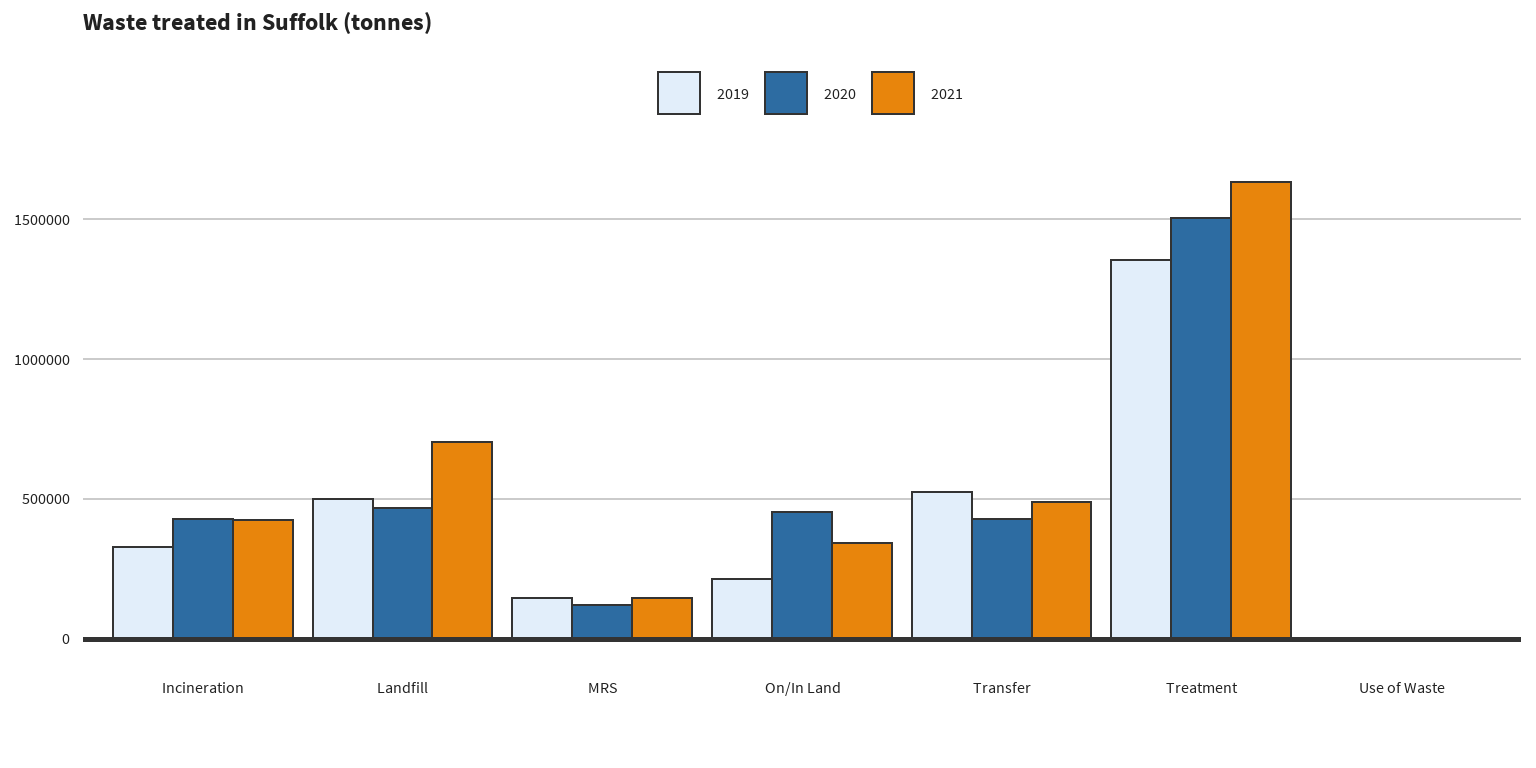
\includegraphics{index_files/figure-latex/wastecapacityplot-1.pdf}
\caption{Source:
\href{https://find-data-beta.cloudapps.digital/dataset/d409b2ba-796c-4436-82c7-eb1831a9ef25/2019-waste-data-interrogator}{Waste
Data Interrogator 2019},
\href{https://www.data.gov.uk/dataset/bb40d091-a346-4b75-aa54-df7d347bed93/2020-waste-data-interrogator}{2020}
and
\href{https://www.data.gov.uk/dataset/d8a12b93-03ef-4fbf-9a43-1ca7a054479c/2021-waste-data-interrogator}{2021}.}
\end{figure}

\hypertarget{waste-to-anaerobic-digestion}{%
\subsubsection{Waste to Anaerobic
Digestion}\label{waste-to-anaerobic-digestion}}

Following on from the Case Study: Food Waste Collection, current
anaerobic digestion treatment in Suffolk is presented in Table
@ref(tab:tabad).

\providecommand{\docline}[3]{\noalign{\global\setlength{\arrayrulewidth}{#1}}\arrayrulecolor[HTML]{#2}\cline{#3}}

\setlength{\tabcolsep}{0pt}

\renewcommand*{\arraystretch}{1.5}

\begin{longtable}[c]{cccc}

\caption{\textcolor[HTML]{000000}{\fontsize{11}{13}\selectfont{Source:\ [Waste\ Data\ Interrogator\ 2019](https://find-data-beta.cloudapps.digital/dataset/d409b2ba-796c-4436-82c7-eb1831a9ef25/2019-waste-data-interrogator),\ [2020](https://www.data.gov.uk/dataset/bb40d091-a346-4b75-aa54-df7d347bed93/2020-waste-data-interrogator)\ and\ [2021](https://www.data.gov.uk/dataset/d8a12b93-03ef-4fbf-9a43-1ca7a054479c/2021-waste-data-interrogator).}}}\\

\hhline{>{\arrayrulecolor[HTML]{666666}\global\arrayrulewidth=2pt}->{\arrayrulecolor[HTML]{666666}\global\arrayrulewidth=2pt}->{\arrayrulecolor[HTML]{666666}\global\arrayrulewidth=2pt}->{\arrayrulecolor[HTML]{666666}\global\arrayrulewidth=2pt}-}

\multicolumn{4}{!{\color[HTML]{000000}\vrule width 0pt}>{}l!{\color[HTML]{000000}\vrule width 0pt}}{\textcolor[HTML]{000000}{\fontsize{11}{11}\selectfont{\textbf{Waste\ treated\ in\ anaerobic\ digestion\ plants\ in\ Suffolk\ in\ 2019,\ 2020\ and\ 2021\ (tonnes)}}}} \\

\hhline{>{\arrayrulecolor[HTML]{666666}\global\arrayrulewidth=0.5pt}->{\arrayrulecolor[HTML]{666666}\global\arrayrulewidth=0.5pt}->{\arrayrulecolor[HTML]{666666}\global\arrayrulewidth=0.5pt}->{\arrayrulecolor[HTML]{666666}\global\arrayrulewidth=0.5pt}-}



\multicolumn{1}{!{\color[HTML]{000000}\vrule width 0pt}>{}l}{\textcolor[HTML]{000000}{\fontsize{11}{11}\selectfont{\textbf{Site\ Name}}}} & \multicolumn{1}{!{\color[HTML]{000000}\vrule width 0pt}>{}l}{\textcolor[HTML]{000000}{\fontsize{11}{11}\selectfont{\textbf{2019}}}} & \multicolumn{1}{!{\color[HTML]{000000}\vrule width 0pt}>{}l}{\textcolor[HTML]{000000}{\fontsize{11}{11}\selectfont{\textbf{2020}}}} & \multicolumn{1}{!{\color[HTML]{000000}\vrule width 0pt}>{}l!{\color[HTML]{000000}\vrule width 0pt}}{\textcolor[HTML]{000000}{\fontsize{11}{11}\selectfont{\textbf{2021}}}} \\

\hhline{>{\arrayrulecolor[HTML]{666666}\global\arrayrulewidth=2pt}->{\arrayrulecolor[HTML]{666666}\global\arrayrulewidth=2pt}->{\arrayrulecolor[HTML]{666666}\global\arrayrulewidth=2pt}->{\arrayrulecolor[HTML]{666666}\global\arrayrulewidth=2pt}-}\endhead



\multicolumn{1}{!{\color[HTML]{000000}\vrule width 0pt}>{}l}{\textcolor[HTML]{000000}{\fontsize{11}{11}\selectfont{Barley\ Brigg\ Biogas\ Ltd}}} & \multicolumn{1}{!{\color[HTML]{000000}\vrule width 0pt}>{}l}{\textcolor[HTML]{000000}{\fontsize{11}{11}\selectfont{16,434}}} & \multicolumn{1}{!{\color[HTML]{000000}\vrule width 0pt}>{}l}{\textcolor[HTML]{000000}{\fontsize{11}{11}\selectfont{15,348}}} & \multicolumn{1}{!{\color[HTML]{000000}\vrule width 0pt}>{}l!{\color[HTML]{000000}\vrule width 0pt}}{\textcolor[HTML]{000000}{\fontsize{11}{11}\selectfont{16,385}}} \\

\hhline{>{\arrayrulecolor[HTML]{666666}\global\arrayrulewidth=0.5pt}->{\arrayrulecolor[HTML]{666666}\global\arrayrulewidth=0.5pt}->{\arrayrulecolor[HTML]{666666}\global\arrayrulewidth=0.5pt}->{\arrayrulecolor[HTML]{666666}\global\arrayrulewidth=0.5pt}-}



\multicolumn{1}{!{\color[HTML]{000000}\vrule width 0pt}>{}l}{\textcolor[HTML]{000000}{\fontsize{11}{11}\selectfont{Bay\ Farm\ AD\ Site\ -\ EPR/JP3900BT}}} & \multicolumn{1}{!{\color[HTML]{000000}\vrule width 0pt}>{}l}{\textcolor[HTML]{000000}{\fontsize{11}{11}\selectfont{\ 2,162}}} & \multicolumn{1}{!{\color[HTML]{000000}\vrule width 0pt}>{}l}{\textcolor[HTML]{000000}{\fontsize{11}{11}\selectfont{\ 8,233}}} & \multicolumn{1}{!{\color[HTML]{000000}\vrule width 0pt}>{}l!{\color[HTML]{000000}\vrule width 0pt}}{\textcolor[HTML]{000000}{\fontsize{11}{11}\selectfont{\ 7,622}}} \\

\hhline{>{\arrayrulecolor[HTML]{666666}\global\arrayrulewidth=0.5pt}->{\arrayrulecolor[HTML]{666666}\global\arrayrulewidth=0.5pt}->{\arrayrulecolor[HTML]{666666}\global\arrayrulewidth=0.5pt}->{\arrayrulecolor[HTML]{666666}\global\arrayrulewidth=0.5pt}-}



\multicolumn{1}{!{\color[HTML]{000000}\vrule width 0pt}>{}l}{\textcolor[HTML]{000000}{\fontsize{11}{11}\selectfont{Bay\ Farm\ AD\ Site\ EPR/WP3433QC}}} & \multicolumn{1}{!{\color[HTML]{000000}\vrule width 0pt}>{}l}{\textcolor[HTML]{000000}{\fontsize{11}{11}\selectfont{\ 7,515}}} & \multicolumn{1}{!{\color[HTML]{000000}\vrule width 0pt}>{}l}{\textcolor[HTML]{000000}{\fontsize{11}{11}\selectfont{\ \ \ \ \ 0}}} & \multicolumn{1}{!{\color[HTML]{000000}\vrule width 0pt}>{}l!{\color[HTML]{000000}\vrule width 0pt}}{\textcolor[HTML]{000000}{\fontsize{11}{11}\selectfont{\ \ \ \ \ 0}}} \\

\hhline{>{\arrayrulecolor[HTML]{666666}\global\arrayrulewidth=0.5pt}->{\arrayrulecolor[HTML]{666666}\global\arrayrulewidth=0.5pt}->{\arrayrulecolor[HTML]{666666}\global\arrayrulewidth=0.5pt}->{\arrayrulecolor[HTML]{666666}\global\arrayrulewidth=0.5pt}-}



\multicolumn{1}{!{\color[HTML]{000000}\vrule width 0pt}>{}l}{\textcolor[HTML]{000000}{\fontsize{11}{11}\selectfont{Symonds\ Farm\ Anaerobic\ Digestion\ Plant}}} & \multicolumn{1}{!{\color[HTML]{000000}\vrule width 0pt}>{}l}{\textcolor[HTML]{000000}{\fontsize{11}{11}\selectfont{\ \ \ 223}}} & \multicolumn{1}{!{\color[HTML]{000000}\vrule width 0pt}>{}l}{\textcolor[HTML]{000000}{\fontsize{11}{11}\selectfont{\ \ \ 889}}} & \multicolumn{1}{!{\color[HTML]{000000}\vrule width 0pt}>{}l!{\color[HTML]{000000}\vrule width 0pt}}{\textcolor[HTML]{000000}{\fontsize{11}{11}\selectfont{\ \ \ 591}}} \\

\hhline{>{\arrayrulecolor[HTML]{666666}\global\arrayrulewidth=2pt}->{\arrayrulecolor[HTML]{666666}\global\arrayrulewidth=2pt}->{\arrayrulecolor[HTML]{666666}\global\arrayrulewidth=2pt}->{\arrayrulecolor[HTML]{666666}\global\arrayrulewidth=2pt}-}



\end{longtable}

The tonnage of waste treated in 2021, totals \textbf{24,597t}. All waste
treated here is classed as ``animal faeces, urine and manure (including
spoiled straw), effluent, collected separately and treated off-site''.
These sites therefore do not currently accept municipal food waste, nor
may they be suitable to do so.

\hypertarget{waste-to-landfill}{%
\subsection{Waste to Landfill}\label{waste-to-landfill}}

Figure @ref(fig:wastetolandfill) shows active Landfill sites. There is
only one active landfill site receiving non-hazardous waste in Suffolk
and this is Masons Landfill site which is operated by Valencia Waste
Management.

Other large recipients of waste to landfill are Shrublands Quarry and
Lawn Farm Quarry, both of which receive significant quantities of inert
waste.

\begin{figure}
\centering
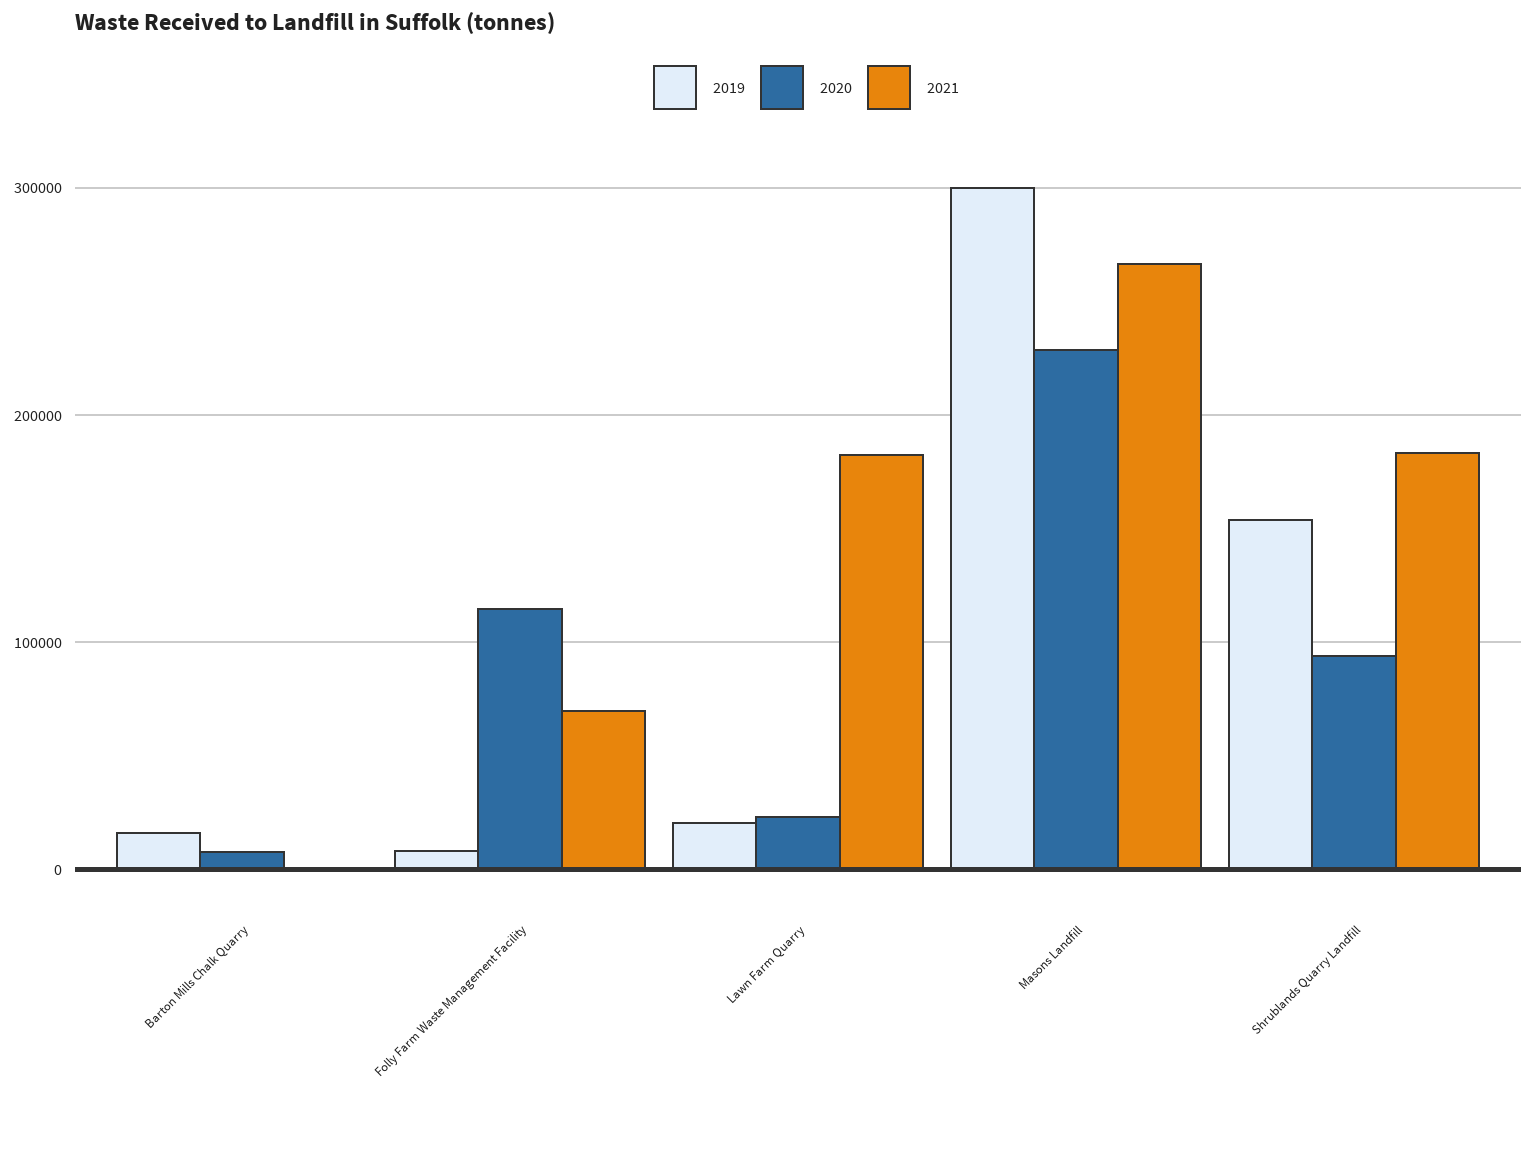
\includegraphics{index_files/figure-latex/wastetolandfill-1.pdf}
\caption{Source:
\href{https://find-data-beta.cloudapps.digital/dataset/d409b2ba-796c-4436-82c7-eb1831a9ef25/2019-waste-data-interrogator}{Waste
Data Interrogator 2019},
\href{https://www.data.gov.uk/dataset/bb40d091-a346-4b75-aa54-df7d347bed93/2020-waste-data-interrogator}{2020}
and
\href{https://www.data.gov.uk/dataset/d8a12b93-03ef-4fbf-9a43-1ca7a054479c/2021-waste-data-interrogator}{2021}.}
\end{figure}

\hypertarget{remaining-landfill-capacity}{%
\subsection{Remaining landfill
capacity}\label{remaining-landfill-capacity}}

Permitted landfill operators have a condition in their permits to report
the remaining landfill void (capacity) of their sites at the end of the
calendar year. Operators can claim commercial confidentiality. See Table
@ref(tab:tablc)

\providecommand{\docline}[3]{\noalign{\global\setlength{\arrayrulewidth}{#1}}\arrayrulecolor[HTML]{#2}\cline{#3}}

\setlength{\tabcolsep}{0pt}

\renewcommand*{\arraystretch}{1.5}

\begin{longtable}[c]{cccccc}

\caption{\textcolor[HTML]{000000}{\fontsize{11}{13}\selectfont{Source:\ [Remaining\ Landfill\ Capacity\ 2019,\ 2020\ and\ 2021.](https://www.data.gov.uk/dataset/237825cb-dc10-4c53-8446-1bcd35614c12/remaining-landfill-capacity)}}}\\

\hhline{>{\arrayrulecolor[HTML]{666666}\global\arrayrulewidth=2pt}->{\arrayrulecolor[HTML]{666666}\global\arrayrulewidth=2pt}->{\arrayrulecolor[HTML]{666666}\global\arrayrulewidth=2pt}->{\arrayrulecolor[HTML]{666666}\global\arrayrulewidth=2pt}->{\arrayrulecolor[HTML]{666666}\global\arrayrulewidth=2pt}->{\arrayrulecolor[HTML]{666666}\global\arrayrulewidth=2pt}-}

\multicolumn{6}{!{\color[HTML]{000000}\vrule width 0pt}>{}l!{\color[HTML]{000000}\vrule width 0pt}}{\textcolor[HTML]{000000}{\fontsize{11}{11}\selectfont{\textbf{Remaining\ landfill\ capacity\ reported\ in\ Suffolk\ (cubic\ metres)}}}} \\

\hhline{>{\arrayrulecolor[HTML]{666666}\global\arrayrulewidth=0.5pt}->{\arrayrulecolor[HTML]{666666}\global\arrayrulewidth=0.5pt}->{\arrayrulecolor[HTML]{666666}\global\arrayrulewidth=0.5pt}->{\arrayrulecolor[HTML]{666666}\global\arrayrulewidth=0.5pt}->{\arrayrulecolor[HTML]{666666}\global\arrayrulewidth=0.5pt}->{\arrayrulecolor[HTML]{666666}\global\arrayrulewidth=0.5pt}-}



\multicolumn{1}{!{\color[HTML]{000000}\vrule width 0pt}>{}l}{\textcolor[HTML]{000000}{\fontsize{11}{11}\selectfont{\textbf{Operator}}}} & \multicolumn{1}{!{\color[HTML]{000000}\vrule width 0pt}>{}l}{\textcolor[HTML]{000000}{\fontsize{11}{11}\selectfont{\textbf{Facility}}}} & \multicolumn{1}{!{\color[HTML]{000000}\vrule width 0pt}>{}l}{\textcolor[HTML]{000000}{\fontsize{11}{11}\selectfont{\textbf{Site\ Type}}}} & \multicolumn{1}{!{\color[HTML]{000000}\vrule width 0pt}>{}r}{\textcolor[HTML]{000000}{\fontsize{11}{11}\selectfont{\textbf{2019}}}} & \multicolumn{1}{!{\color[HTML]{000000}\vrule width 0pt}>{}r}{\textcolor[HTML]{000000}{\fontsize{11}{11}\selectfont{\textbf{2020}}}} & \multicolumn{1}{!{\color[HTML]{000000}\vrule width 0pt}>{}r!{\color[HTML]{000000}\vrule width 0pt}}{\textcolor[HTML]{000000}{\fontsize{11}{11}\selectfont{\textbf{2021}}}} \\

\hhline{>{\arrayrulecolor[HTML]{666666}\global\arrayrulewidth=2pt}->{\arrayrulecolor[HTML]{666666}\global\arrayrulewidth=2pt}->{\arrayrulecolor[HTML]{666666}\global\arrayrulewidth=2pt}->{\arrayrulecolor[HTML]{666666}\global\arrayrulewidth=2pt}->{\arrayrulecolor[HTML]{666666}\global\arrayrulewidth=2pt}->{\arrayrulecolor[HTML]{666666}\global\arrayrulewidth=2pt}-}\endhead



\multicolumn{1}{!{\color[HTML]{000000}\vrule width 0pt}>{}l}{\textcolor[HTML]{000000}{\fontsize{11}{11}\selectfont{Brett\ Aggregates\ Ltd}}} & \multicolumn{1}{!{\color[HTML]{000000}\vrule width 0pt}>{}l}{\textcolor[HTML]{000000}{\fontsize{11}{11}\selectfont{Shrublands\ Quarry}}} & \multicolumn{1}{!{\color[HTML]{000000}\vrule width 0pt}>{}l}{\textcolor[HTML]{000000}{\fontsize{11}{11}\selectfont{L05\ -\ Inert\ Landfill}}} & \multicolumn{1}{!{\color[HTML]{000000}\vrule width 0pt}>{}r}{\textcolor[HTML]{000000}{\fontsize{11}{11}\selectfont{771,500}}} & \multicolumn{1}{!{\color[HTML]{000000}\vrule width 0pt}>{}r}{\textcolor[HTML]{000000}{\fontsize{11}{11}\selectfont{634,934}}} & \multicolumn{1}{!{\color[HTML]{000000}\vrule width 0pt}>{}r!{\color[HTML]{000000}\vrule width 0pt}}{\textcolor[HTML]{000000}{\fontsize{11}{11}\selectfont{532,650}}} \\

\hhline{>{\arrayrulecolor[HTML]{666666}\global\arrayrulewidth=0.5pt}->{\arrayrulecolor[HTML]{666666}\global\arrayrulewidth=0.5pt}->{\arrayrulecolor[HTML]{666666}\global\arrayrulewidth=0.5pt}->{\arrayrulecolor[HTML]{666666}\global\arrayrulewidth=0.5pt}->{\arrayrulecolor[HTML]{666666}\global\arrayrulewidth=0.5pt}->{\arrayrulecolor[HTML]{666666}\global\arrayrulewidth=0.5pt}-}



\multicolumn{1}{!{\color[HTML]{000000}\vrule width 0pt}>{}l}{\textcolor[HTML]{000000}{\fontsize{11}{11}\selectfont{Aggmax\ Ltd}}} & \multicolumn{1}{!{\color[HTML]{000000}\vrule width 0pt}>{}l}{\textcolor[HTML]{000000}{\fontsize{11}{11}\selectfont{Lawn\ Farm\ Quarry}}} & \multicolumn{1}{!{\color[HTML]{000000}\vrule width 0pt}>{}l}{\textcolor[HTML]{000000}{\fontsize{11}{11}\selectfont{L05\ -\ Inert\ Landfill}}} & \multicolumn{1}{!{\color[HTML]{000000}\vrule width 0pt}>{}r}{\textcolor[HTML]{000000}{\fontsize{11}{11}\selectfont{1,330,000}}} & \multicolumn{1}{!{\color[HTML]{000000}\vrule width 0pt}>{}r}{\textcolor[HTML]{000000}{\fontsize{11}{11}\selectfont{1,330,000}}} & \multicolumn{1}{!{\color[HTML]{000000}\vrule width 0pt}>{}r!{\color[HTML]{000000}\vrule width 0pt}}{\textcolor[HTML]{000000}{\fontsize{11}{11}\selectfont{1,330,000}}} \\

\hhline{>{\arrayrulecolor[HTML]{666666}\global\arrayrulewidth=0.5pt}->{\arrayrulecolor[HTML]{666666}\global\arrayrulewidth=0.5pt}->{\arrayrulecolor[HTML]{666666}\global\arrayrulewidth=0.5pt}->{\arrayrulecolor[HTML]{666666}\global\arrayrulewidth=0.5pt}->{\arrayrulecolor[HTML]{666666}\global\arrayrulewidth=0.5pt}->{\arrayrulecolor[HTML]{666666}\global\arrayrulewidth=0.5pt}-}



\multicolumn{1}{!{\color[HTML]{000000}\vrule width 0pt}>{}l}{\textcolor[HTML]{000000}{\fontsize{11}{11}\selectfont{Cemex\ Uk\ Materials\ Ltd}}} & \multicolumn{1}{!{\color[HTML]{000000}\vrule width 0pt}>{}l}{\textcolor[HTML]{000000}{\fontsize{11}{11}\selectfont{Cartwrights\ Covert\ Landfill}}} & \multicolumn{1}{!{\color[HTML]{000000}\vrule width 0pt}>{}l}{\textcolor[HTML]{000000}{\fontsize{11}{11}\selectfont{L05\ -\ Inert\ Landfill}}} & \multicolumn{1}{!{\color[HTML]{000000}\vrule width 0pt}>{}r}{\textcolor[HTML]{000000}{\fontsize{11}{11}\selectfont{178,000}}} & \multicolumn{1}{!{\color[HTML]{000000}\vrule width 0pt}>{}r}{\textcolor[HTML]{000000}{\fontsize{11}{11}\selectfont{178,000}}} & \multicolumn{1}{!{\color[HTML]{000000}\vrule width 0pt}>{}r!{\color[HTML]{000000}\vrule width 0pt}}{\textcolor[HTML]{000000}{\fontsize{11}{11}\selectfont{178,000}}} \\

\hhline{>{\arrayrulecolor[HTML]{666666}\global\arrayrulewidth=0.5pt}->{\arrayrulecolor[HTML]{666666}\global\arrayrulewidth=0.5pt}->{\arrayrulecolor[HTML]{666666}\global\arrayrulewidth=0.5pt}->{\arrayrulecolor[HTML]{666666}\global\arrayrulewidth=0.5pt}->{\arrayrulecolor[HTML]{666666}\global\arrayrulewidth=0.5pt}->{\arrayrulecolor[HTML]{666666}\global\arrayrulewidth=0.5pt}-}



\multicolumn{1}{!{\color[HTML]{000000}\vrule width 0pt}>{}l}{\textcolor[HTML]{000000}{\fontsize{11}{11}\selectfont{Sewells\ Reservoir\ Construction\ Ltd}}} & \multicolumn{1}{!{\color[HTML]{000000}\vrule width 0pt}>{}l}{\textcolor[HTML]{000000}{\fontsize{11}{11}\selectfont{Barton\ Mills\ Chalk\ Quarry}}} & \multicolumn{1}{!{\color[HTML]{000000}\vrule width 0pt}>{}l}{\textcolor[HTML]{000000}{\fontsize{11}{11}\selectfont{L05\ -\ Inert\ Landfill}}} & \multicolumn{1}{!{\color[HTML]{000000}\vrule width 0pt}>{}r}{\textcolor[HTML]{000000}{\fontsize{11}{11}\selectfont{1,050,000}}} & \multicolumn{1}{!{\color[HTML]{000000}\vrule width 0pt}>{}r}{\textcolor[HTML]{000000}{\fontsize{11}{11}\selectfont{1,050,000}}} & \multicolumn{1}{!{\color[HTML]{000000}\vrule width 0pt}>{}r!{\color[HTML]{000000}\vrule width 0pt}}{\textcolor[HTML]{000000}{\fontsize{11}{11}\selectfont{1,050,000}}} \\

\hhline{>{\arrayrulecolor[HTML]{666666}\global\arrayrulewidth=0.5pt}->{\arrayrulecolor[HTML]{666666}\global\arrayrulewidth=0.5pt}->{\arrayrulecolor[HTML]{666666}\global\arrayrulewidth=0.5pt}->{\arrayrulecolor[HTML]{666666}\global\arrayrulewidth=0.5pt}->{\arrayrulecolor[HTML]{666666}\global\arrayrulewidth=0.5pt}->{\arrayrulecolor[HTML]{666666}\global\arrayrulewidth=0.5pt}-}



\multicolumn{1}{!{\color[HTML]{000000}\vrule width 0pt}>{}l}{\textcolor[HTML]{000000}{\fontsize{11}{11}\selectfont{Viridor\ Waste\ Management\ Ltd}}} & \multicolumn{1}{!{\color[HTML]{000000}\vrule width 0pt}>{}l}{\textcolor[HTML]{000000}{\fontsize{11}{11}\selectfont{MASONS\ LANDFILL}}} & \multicolumn{1}{!{\color[HTML]{000000}\vrule width 0pt}>{}l}{\textcolor[HTML]{000000}{\fontsize{11}{11}\selectfont{L02\ -\ Non\ Hazardous\ Landfill\ With\ SNRHW\ cell}}} & \multicolumn{1}{!{\color[HTML]{000000}\vrule width 0pt}>{}r}{\textcolor[HTML]{000000}{\fontsize{11}{11}\selectfont{2,490,000}}} & \multicolumn{1}{!{\color[HTML]{000000}\vrule width 0pt}>{}r}{\textcolor[HTML]{000000}{\fontsize{11}{11}\selectfont{2,839,864}}} & \multicolumn{1}{!{\color[HTML]{000000}\vrule width 0pt}>{}r!{\color[HTML]{000000}\vrule width 0pt}}{\textcolor[HTML]{000000}{\fontsize{11}{11}\selectfont{2,604,173}}} \\

\hhline{>{\arrayrulecolor[HTML]{666666}\global\arrayrulewidth=0.5pt}->{\arrayrulecolor[HTML]{666666}\global\arrayrulewidth=0.5pt}->{\arrayrulecolor[HTML]{666666}\global\arrayrulewidth=0.5pt}->{\arrayrulecolor[HTML]{666666}\global\arrayrulewidth=0.5pt}->{\arrayrulecolor[HTML]{666666}\global\arrayrulewidth=0.5pt}->{\arrayrulecolor[HTML]{666666}\global\arrayrulewidth=0.5pt}-}



\multicolumn{1}{!{\color[HTML]{000000}\vrule width 0pt}>{}l}{\textcolor[HTML]{000000}{\fontsize{11}{11}\selectfont{Shotley\ Holdings\ Ltd}}} & \multicolumn{1}{!{\color[HTML]{000000}\vrule width 0pt}>{}l}{\textcolor[HTML]{000000}{\fontsize{11}{11}\selectfont{Folly\ Farm\ Landfill}}} & \multicolumn{1}{!{\color[HTML]{000000}\vrule width 0pt}>{}l}{\textcolor[HTML]{000000}{\fontsize{11}{11}\selectfont{L02\ -\ Non\ Hazardous\ Landfill\ With\ SNRHW\ cell}}} & \multicolumn{1}{!{\color[HTML]{000000}\vrule width 0pt}>{}r}{\textcolor[HTML]{000000}{\fontsize{11}{11}\selectfont{575,639}}} & \multicolumn{1}{!{\color[HTML]{000000}\vrule width 0pt}>{}r}{\textcolor[HTML]{000000}{\fontsize{11}{11}\selectfont{561,222}}} & \multicolumn{1}{!{\color[HTML]{000000}\vrule width 0pt}>{}r!{\color[HTML]{000000}\vrule width 0pt}}{\textcolor[HTML]{000000}{\fontsize{11}{11}\selectfont{474,946}}} \\

\hhline{>{\arrayrulecolor[HTML]{666666}\global\arrayrulewidth=2pt}->{\arrayrulecolor[HTML]{666666}\global\arrayrulewidth=2pt}->{\arrayrulecolor[HTML]{666666}\global\arrayrulewidth=2pt}->{\arrayrulecolor[HTML]{666666}\global\arrayrulewidth=2pt}->{\arrayrulecolor[HTML]{666666}\global\arrayrulewidth=2pt}->{\arrayrulecolor[HTML]{666666}\global\arrayrulewidth=2pt}-}



\end{longtable}

In Figure @ref(fig:landfillcapacityplot) Landfill capacity change is
shown between 2019 and 2021, for sites where there is capacity.

\begin{figure}
\centering
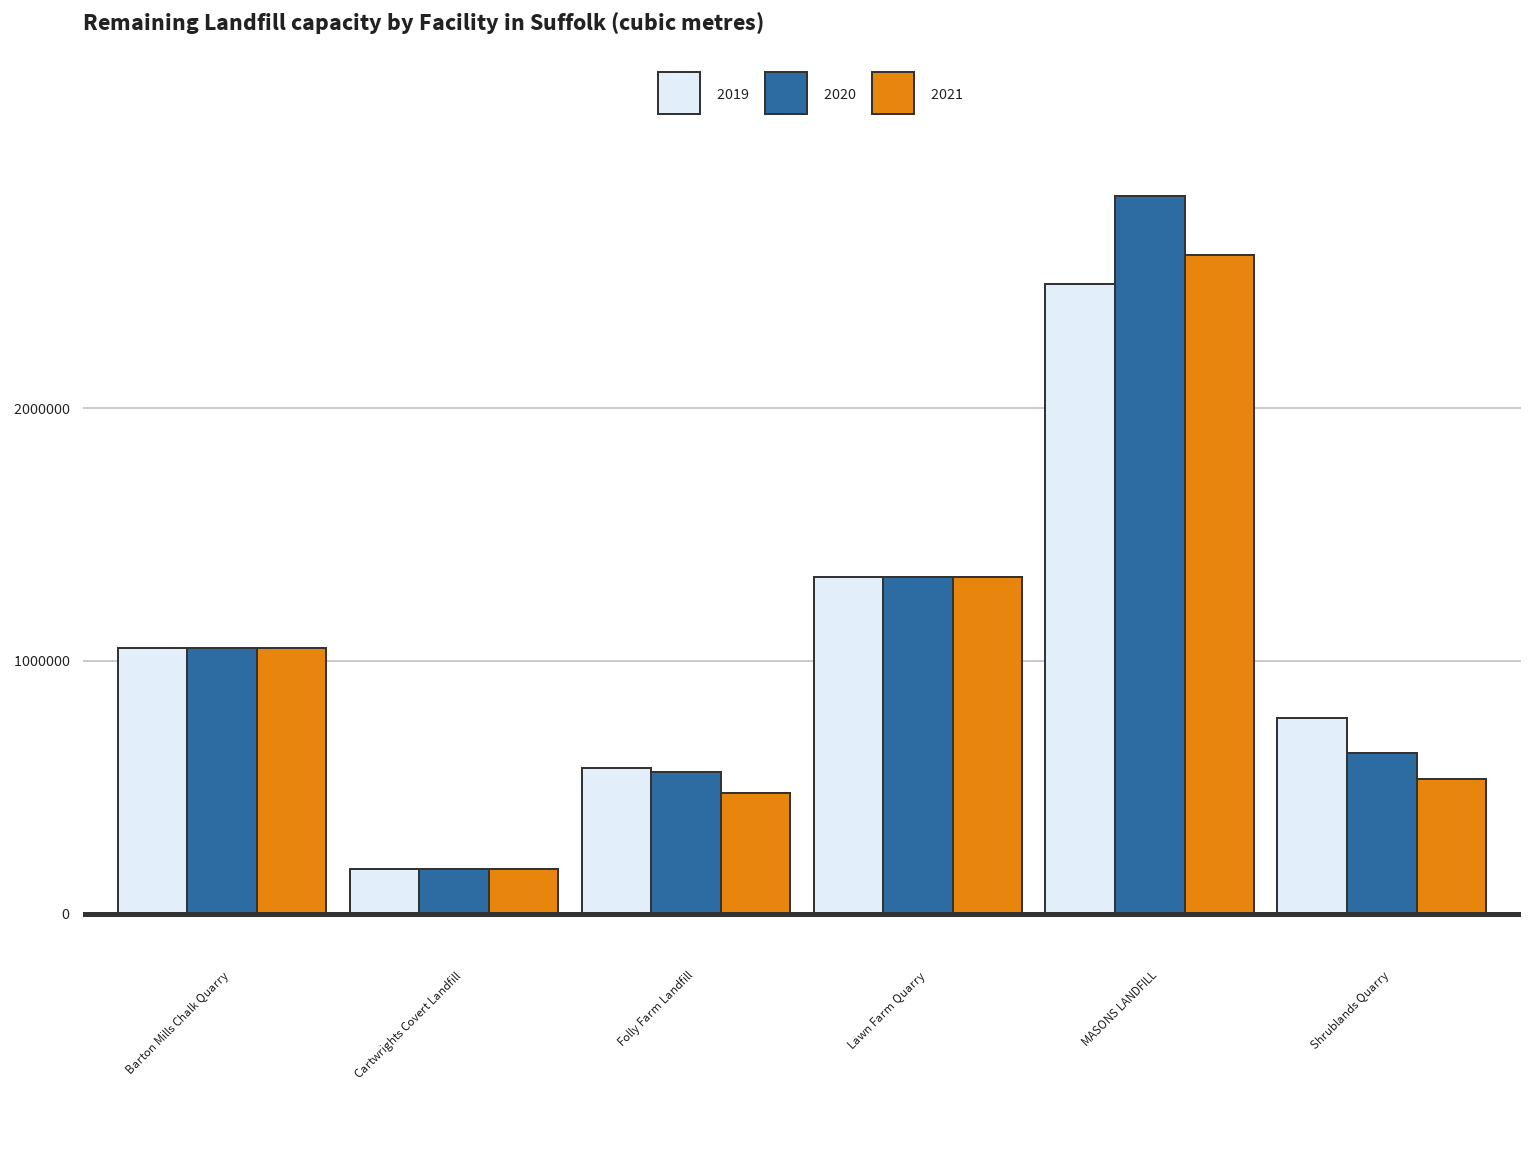
\includegraphics{index_files/figure-latex/landfillcapacityplot-1.pdf}
\caption{Source:
\href{https://www.data.gov.uk/dataset/237825cb-dc10-4c53-8446-1bcd35614c12/remaining-landfill-capacity}{Remaining
Landfill Capacity 2019, 2020 and 2021}}
\end{figure}

\newpage

\hypertarget{waste-movements}{%
\section{Waste Movements}\label{waste-movements}}

\hypertarget{waste-managed-in-suffolk-from-other-waste-planning-authorities}{%
\subsection{Waste Managed in Suffolk from other Waste Planning
Authorities}\label{waste-managed-in-suffolk-from-other-waste-planning-authorities}}

To determine whether Suffolk achieves its goal of net self-sufficiency
in the management of waste arising wihin the Plan Area, we can look at
the movement of waste in and out of the County.

Table @ref(tab:tab1) shows all waste managed in Suffolk, and the Waste
Planning Authority (WPA) from which the waste originated. It shows the
figures for Suffolk, all our nearest neighbours, as well as `All Other
WPAs' combined.

\providecommand{\docline}[3]{\noalign{\global\setlength{\arrayrulewidth}{#1}}\arrayrulecolor[HTML]{#2}\cline{#3}}

\setlength{\tabcolsep}{0pt}

\renewcommand*{\arraystretch}{1.5}

\begin{longtable}[c]{cccc}

\caption{\textcolor[HTML]{000000}{\fontsize{11}{13}\selectfont{Source:\ [Waste\ Data\ Interrogator\ 2019](https://find-data-beta.cloudapps.digital/dataset/d409b2ba-796c-4436-82c7-eb1831a9ef25/2019-waste-data-interrogator),\ [2020](https://www.data.gov.uk/dataset/bb40d091-a346-4b75-aa54-df7d347bed93/2020-waste-data-interrogator)\ and\ [2021](https://www.data.gov.uk/dataset/d8a12b93-03ef-4fbf-9a43-1ca7a054479c/2021-waste-data-interrogator).}}}\\

\hhline{>{\arrayrulecolor[HTML]{666666}\global\arrayrulewidth=2pt}->{\arrayrulecolor[HTML]{666666}\global\arrayrulewidth=2pt}->{\arrayrulecolor[HTML]{666666}\global\arrayrulewidth=2pt}->{\arrayrulecolor[HTML]{666666}\global\arrayrulewidth=2pt}-}

\multicolumn{4}{!{\color[HTML]{000000}\vrule width 0pt}>{}l!{\color[HTML]{000000}\vrule width 0pt}}{\textcolor[HTML]{000000}{\fontsize{11}{11}\selectfont{\textbf{All\ waste\ managed\ in\ Suffolk\ (tonnes)}}}} \\

\hhline{>{\arrayrulecolor[HTML]{666666}\global\arrayrulewidth=0.5pt}->{\arrayrulecolor[HTML]{666666}\global\arrayrulewidth=0.5pt}->{\arrayrulecolor[HTML]{666666}\global\arrayrulewidth=0.5pt}->{\arrayrulecolor[HTML]{666666}\global\arrayrulewidth=0.5pt}-}



\multicolumn{1}{!{\color[HTML]{000000}\vrule width 0pt}>{}l}{\textcolor[HTML]{000000}{\fontsize{11}{11}\selectfont{\textbf{Origin\ WPA}}}} & \multicolumn{1}{!{\color[HTML]{000000}\vrule width 0pt}>{}l}{\textcolor[HTML]{000000}{\fontsize{11}{11}\selectfont{\textbf{2019}}}} & \multicolumn{1}{!{\color[HTML]{000000}\vrule width 0pt}>{}l}{\textcolor[HTML]{000000}{\fontsize{11}{11}\selectfont{\textbf{2020}}}} & \multicolumn{1}{!{\color[HTML]{000000}\vrule width 0pt}>{}l!{\color[HTML]{000000}\vrule width 0pt}}{\textcolor[HTML]{000000}{\fontsize{11}{11}\selectfont{\textbf{2021}}}} \\

\hhline{>{\arrayrulecolor[HTML]{666666}\global\arrayrulewidth=2pt}->{\arrayrulecolor[HTML]{666666}\global\arrayrulewidth=2pt}->{\arrayrulecolor[HTML]{666666}\global\arrayrulewidth=2pt}->{\arrayrulecolor[HTML]{666666}\global\arrayrulewidth=2pt}-}\endhead



\multicolumn{1}{!{\color[HTML]{000000}\vrule width 0pt}>{}l}{\textcolor[HTML]{000000}{\fontsize{11}{11}\selectfont{Suffolk}}} & \multicolumn{1}{!{\color[HTML]{000000}\vrule width 0pt}>{}l}{\textcolor[HTML]{000000}{\fontsize{11}{11}\selectfont{2,331,864}}} & \multicolumn{1}{!{\color[HTML]{000000}\vrule width 0pt}>{}l}{\textcolor[HTML]{000000}{\fontsize{11}{11}\selectfont{2,457,668}}} & \multicolumn{1}{!{\color[HTML]{000000}\vrule width 0pt}>{}l!{\color[HTML]{000000}\vrule width 0pt}}{\textcolor[HTML]{000000}{\fontsize{11}{11}\selectfont{2,737,551}}} \\

\hhline{>{\arrayrulecolor[HTML]{666666}\global\arrayrulewidth=0.5pt}->{\arrayrulecolor[HTML]{666666}\global\arrayrulewidth=0.5pt}->{\arrayrulecolor[HTML]{666666}\global\arrayrulewidth=0.5pt}->{\arrayrulecolor[HTML]{666666}\global\arrayrulewidth=0.5pt}-}



\multicolumn{1}{!{\color[HTML]{000000}\vrule width 0pt}>{}l}{\textcolor[HTML]{000000}{\fontsize{11}{11}\selectfont{Norfolk}}} & \multicolumn{1}{!{\color[HTML]{000000}\vrule width 0pt}>{}l}{\textcolor[HTML]{000000}{\fontsize{11}{11}\selectfont{\ \ 216,900}}} & \multicolumn{1}{!{\color[HTML]{000000}\vrule width 0pt}>{}l}{\textcolor[HTML]{000000}{\fontsize{11}{11}\selectfont{\ \ 274,238}}} & \multicolumn{1}{!{\color[HTML]{000000}\vrule width 0pt}>{}l!{\color[HTML]{000000}\vrule width 0pt}}{\textcolor[HTML]{000000}{\fontsize{11}{11}\selectfont{\ \ 355,742}}} \\

\hhline{>{\arrayrulecolor[HTML]{666666}\global\arrayrulewidth=0.5pt}->{\arrayrulecolor[HTML]{666666}\global\arrayrulewidth=0.5pt}->{\arrayrulecolor[HTML]{666666}\global\arrayrulewidth=0.5pt}->{\arrayrulecolor[HTML]{666666}\global\arrayrulewidth=0.5pt}-}



\multicolumn{1}{!{\color[HTML]{000000}\vrule width 0pt}>{}l}{\textcolor[HTML]{000000}{\fontsize{11}{11}\selectfont{Essex}}} & \multicolumn{1}{!{\color[HTML]{000000}\vrule width 0pt}>{}l}{\textcolor[HTML]{000000}{\fontsize{11}{11}\selectfont{\ \ 184,172}}} & \multicolumn{1}{!{\color[HTML]{000000}\vrule width 0pt}>{}l}{\textcolor[HTML]{000000}{\fontsize{11}{11}\selectfont{\ \ 242,291}}} & \multicolumn{1}{!{\color[HTML]{000000}\vrule width 0pt}>{}l!{\color[HTML]{000000}\vrule width 0pt}}{\textcolor[HTML]{000000}{\fontsize{11}{11}\selectfont{\ \ 288,778}}} \\

\hhline{>{\arrayrulecolor[HTML]{666666}\global\arrayrulewidth=0.5pt}->{\arrayrulecolor[HTML]{666666}\global\arrayrulewidth=0.5pt}->{\arrayrulecolor[HTML]{666666}\global\arrayrulewidth=0.5pt}->{\arrayrulecolor[HTML]{666666}\global\arrayrulewidth=0.5pt}-}



\multicolumn{1}{!{\color[HTML]{000000}\vrule width 0pt}>{}l}{\textcolor[HTML]{000000}{\fontsize{11}{11}\selectfont{\textit{All\ Other\ WPAs}}}} & \multicolumn{1}{!{\color[HTML]{000000}\vrule width 0pt}>{}l}{\textcolor[HTML]{000000}{\fontsize{11}{11}\selectfont{\ \ 382,474}}} & \multicolumn{1}{!{\color[HTML]{000000}\vrule width 0pt}>{}l}{\textcolor[HTML]{000000}{\fontsize{11}{11}\selectfont{\ \ 225,617}}} & \multicolumn{1}{!{\color[HTML]{000000}\vrule width 0pt}>{}l!{\color[HTML]{000000}\vrule width 0pt}}{\textcolor[HTML]{000000}{\fontsize{11}{11}\selectfont{\ \ 211,342}}} \\

\hhline{>{\arrayrulecolor[HTML]{666666}\global\arrayrulewidth=0.5pt}->{\arrayrulecolor[HTML]{666666}\global\arrayrulewidth=0.5pt}->{\arrayrulecolor[HTML]{666666}\global\arrayrulewidth=0.5pt}->{\arrayrulecolor[HTML]{666666}\global\arrayrulewidth=0.5pt}-}



\multicolumn{1}{!{\color[HTML]{000000}\vrule width 0pt}>{}l}{\textcolor[HTML]{000000}{\fontsize{11}{11}\selectfont{Cambridgeshire}}} & \multicolumn{1}{!{\color[HTML]{000000}\vrule width 0pt}>{}l}{\textcolor[HTML]{000000}{\fontsize{11}{11}\selectfont{\ \ \ 87,527}}} & \multicolumn{1}{!{\color[HTML]{000000}\vrule width 0pt}>{}l}{\textcolor[HTML]{000000}{\fontsize{11}{11}\selectfont{\ \ 200,187}}} & \multicolumn{1}{!{\color[HTML]{000000}\vrule width 0pt}>{}l!{\color[HTML]{000000}\vrule width 0pt}}{\textcolor[HTML]{000000}{\fontsize{11}{11}\selectfont{\ \ 140,731}}} \\

\hhline{>{\arrayrulecolor[HTML]{666666}\global\arrayrulewidth=0.5pt}->{\arrayrulecolor[HTML]{666666}\global\arrayrulewidth=0.5pt}->{\arrayrulecolor[HTML]{666666}\global\arrayrulewidth=0.5pt}->{\arrayrulecolor[HTML]{666666}\global\arrayrulewidth=0.5pt}-}



\multicolumn{1}{!{\color[HTML]{000000}\vrule width 0pt}>{}l}{\textcolor[HTML]{000000}{\fontsize{11}{11}\selectfont{\textbf{Total\ waste\ managed\ origin\ outwith\ Suffolk}}}} & \multicolumn{1}{!{\color[HTML]{000000}\vrule width 0pt}>{}l}{\textcolor[HTML]{000000}{\fontsize{11}{11}\selectfont{\textbf{\ \ 871,073}}}} & \multicolumn{1}{!{\color[HTML]{000000}\vrule width 0pt}>{}l}{\textcolor[HTML]{000000}{\fontsize{11}{11}\selectfont{\textbf{\ \ 942,333}}}} & \multicolumn{1}{!{\color[HTML]{000000}\vrule width 0pt}>{}l!{\color[HTML]{000000}\vrule width 0pt}}{\textcolor[HTML]{000000}{\fontsize{11}{11}\selectfont{\textbf{\ \ 996,593}}}} \\

\hhline{>{\arrayrulecolor[HTML]{666666}\global\arrayrulewidth=0.5pt}->{\arrayrulecolor[HTML]{666666}\global\arrayrulewidth=0.5pt}->{\arrayrulecolor[HTML]{666666}\global\arrayrulewidth=0.5pt}->{\arrayrulecolor[HTML]{666666}\global\arrayrulewidth=0.5pt}-}



\multicolumn{1}{!{\color[HTML]{000000}\vrule width 0pt}>{}l}{\textcolor[HTML]{000000}{\fontsize{11}{11}\selectfont{\textbf{Total\ waste\ managed\ in\ Suffolk}}}} & \multicolumn{1}{!{\color[HTML]{000000}\vrule width 0pt}>{}l}{\textcolor[HTML]{000000}{\fontsize{11}{11}\selectfont{\textbf{3,202,937}}}} & \multicolumn{1}{!{\color[HTML]{000000}\vrule width 0pt}>{}l}{\textcolor[HTML]{000000}{\fontsize{11}{11}\selectfont{\textbf{3,400,001}}}} & \multicolumn{1}{!{\color[HTML]{000000}\vrule width 0pt}>{}l!{\color[HTML]{000000}\vrule width 0pt}}{\textcolor[HTML]{000000}{\fontsize{11}{11}\selectfont{\textbf{3,734,144}}}} \\

\hhline{>{\arrayrulecolor[HTML]{666666}\global\arrayrulewidth=2pt}->{\arrayrulecolor[HTML]{666666}\global\arrayrulewidth=2pt}->{\arrayrulecolor[HTML]{666666}\global\arrayrulewidth=2pt}->{\arrayrulecolor[HTML]{666666}\global\arrayrulewidth=2pt}-}



\end{longtable}

Table @ref(tab:tab2) is a further breakdown of Table @ref(tab:tab1)
showing all waste sent to landfill in Suffolk, and the WPA from which
the waste originated.

\providecommand{\docline}[3]{\noalign{\global\setlength{\arrayrulewidth}{#1}}\arrayrulecolor[HTML]{#2}\cline{#3}}

\setlength{\tabcolsep}{0pt}

\renewcommand*{\arraystretch}{1.5}

\begin{longtable}[c]{cccc}

\caption{\textcolor[HTML]{000000}{\fontsize{11}{13}\selectfont{Source:\ [Waste\ Data\ Interrogator\ 2019](https://find-data-beta.cloudapps.digital/dataset/d409b2ba-796c-4436-82c7-eb1831a9ef25/2019-waste-data-interrogator),\ [2020](https://www.data.gov.uk/dataset/bb40d091-a346-4b75-aa54-df7d347bed93/2020-waste-data-interrogator)\ and\ [2021](https://www.data.gov.uk/dataset/d8a12b93-03ef-4fbf-9a43-1ca7a054479c/2021-waste-data-interrogator).}}}\\

\hhline{>{\arrayrulecolor[HTML]{666666}\global\arrayrulewidth=2pt}->{\arrayrulecolor[HTML]{666666}\global\arrayrulewidth=2pt}->{\arrayrulecolor[HTML]{666666}\global\arrayrulewidth=2pt}->{\arrayrulecolor[HTML]{666666}\global\arrayrulewidth=2pt}-}

\multicolumn{4}{!{\color[HTML]{000000}\vrule width 0pt}>{}l!{\color[HTML]{000000}\vrule width 0pt}}{\textcolor[HTML]{000000}{\fontsize{11}{11}\selectfont{\textbf{Waste\ sent\ to\ landfill\ in\ Suffolk\ (tonnes)}}}} \\

\hhline{>{\arrayrulecolor[HTML]{666666}\global\arrayrulewidth=0.5pt}->{\arrayrulecolor[HTML]{666666}\global\arrayrulewidth=0.5pt}->{\arrayrulecolor[HTML]{666666}\global\arrayrulewidth=0.5pt}->{\arrayrulecolor[HTML]{666666}\global\arrayrulewidth=0.5pt}-}



\multicolumn{1}{!{\color[HTML]{000000}\vrule width 0pt}>{}l}{\textcolor[HTML]{000000}{\fontsize{11}{11}\selectfont{\textbf{Origin\ WPA}}}} & \multicolumn{1}{!{\color[HTML]{000000}\vrule width 0pt}>{}l}{\textcolor[HTML]{000000}{\fontsize{11}{11}\selectfont{\textbf{2019}}}} & \multicolumn{1}{!{\color[HTML]{000000}\vrule width 0pt}>{}l}{\textcolor[HTML]{000000}{\fontsize{11}{11}\selectfont{\textbf{2021}}}} & \multicolumn{1}{!{\color[HTML]{000000}\vrule width 0pt}>{}l!{\color[HTML]{000000}\vrule width 0pt}}{\textcolor[HTML]{000000}{\fontsize{11}{11}\selectfont{\textbf{2020}}}} \\

\hhline{>{\arrayrulecolor[HTML]{666666}\global\arrayrulewidth=2pt}->{\arrayrulecolor[HTML]{666666}\global\arrayrulewidth=2pt}->{\arrayrulecolor[HTML]{666666}\global\arrayrulewidth=2pt}->{\arrayrulecolor[HTML]{666666}\global\arrayrulewidth=2pt}-}\endhead



\multicolumn{1}{!{\color[HTML]{000000}\vrule width 0pt}>{}l}{\textcolor[HTML]{000000}{\fontsize{11}{11}\selectfont{Suffolk}}} & \multicolumn{1}{!{\color[HTML]{000000}\vrule width 0pt}>{}l}{\textcolor[HTML]{000000}{\fontsize{11}{11}\selectfont{257,482}}} & \multicolumn{1}{!{\color[HTML]{000000}\vrule width 0pt}>{}l}{\textcolor[HTML]{000000}{\fontsize{11}{11}\selectfont{527,918}}} & \multicolumn{1}{!{\color[HTML]{000000}\vrule width 0pt}>{}l!{\color[HTML]{000000}\vrule width 0pt}}{\textcolor[HTML]{000000}{\fontsize{11}{11}\selectfont{333,376}}} \\

\hhline{>{\arrayrulecolor[HTML]{666666}\global\arrayrulewidth=0.5pt}->{\arrayrulecolor[HTML]{666666}\global\arrayrulewidth=0.5pt}->{\arrayrulecolor[HTML]{666666}\global\arrayrulewidth=0.5pt}->{\arrayrulecolor[HTML]{666666}\global\arrayrulewidth=0.5pt}-}



\multicolumn{1}{!{\color[HTML]{000000}\vrule width 0pt}>{}l}{\textcolor[HTML]{000000}{\fontsize{11}{11}\selectfont{Essex}}} & \multicolumn{1}{!{\color[HTML]{000000}\vrule width 0pt}>{}l}{\textcolor[HTML]{000000}{\fontsize{11}{11}\selectfont{\ 37,736}}} & \multicolumn{1}{!{\color[HTML]{000000}\vrule width 0pt}>{}l}{\textcolor[HTML]{000000}{\fontsize{11}{11}\selectfont{121,344}}} & \multicolumn{1}{!{\color[HTML]{000000}\vrule width 0pt}>{}l!{\color[HTML]{000000}\vrule width 0pt}}{\textcolor[HTML]{000000}{\fontsize{11}{11}\selectfont{\ 88,094}}} \\

\hhline{>{\arrayrulecolor[HTML]{666666}\global\arrayrulewidth=0.5pt}->{\arrayrulecolor[HTML]{666666}\global\arrayrulewidth=0.5pt}->{\arrayrulecolor[HTML]{666666}\global\arrayrulewidth=0.5pt}->{\arrayrulecolor[HTML]{666666}\global\arrayrulewidth=0.5pt}-}



\multicolumn{1}{!{\color[HTML]{000000}\vrule width 0pt}>{}l}{\textcolor[HTML]{000000}{\fontsize{11}{11}\selectfont{Norfolk}}} & \multicolumn{1}{!{\color[HTML]{000000}\vrule width 0pt}>{}l}{\textcolor[HTML]{000000}{\fontsize{11}{11}\selectfont{\ 33,210}}} & \multicolumn{1}{!{\color[HTML]{000000}\vrule width 0pt}>{}l}{\textcolor[HTML]{000000}{\fontsize{11}{11}\selectfont{\ 48,907}}} & \multicolumn{1}{!{\color[HTML]{000000}\vrule width 0pt}>{}l!{\color[HTML]{000000}\vrule width 0pt}}{\textcolor[HTML]{000000}{\fontsize{11}{11}\selectfont{\ 40,438}}} \\

\hhline{>{\arrayrulecolor[HTML]{666666}\global\arrayrulewidth=0.5pt}->{\arrayrulecolor[HTML]{666666}\global\arrayrulewidth=0.5pt}->{\arrayrulecolor[HTML]{666666}\global\arrayrulewidth=0.5pt}->{\arrayrulecolor[HTML]{666666}\global\arrayrulewidth=0.5pt}-}



\multicolumn{1}{!{\color[HTML]{000000}\vrule width 0pt}>{}l}{\textcolor[HTML]{000000}{\fontsize{11}{11}\selectfont{\textit{All\ Other\ WPAs}}}} & \multicolumn{1}{!{\color[HTML]{000000}\vrule width 0pt}>{}l}{\textcolor[HTML]{000000}{\fontsize{11}{11}\selectfont{169,004}}} & \multicolumn{1}{!{\color[HTML]{000000}\vrule width 0pt}>{}l}{\textcolor[HTML]{000000}{\fontsize{11}{11}\selectfont{\ \ 4,190}}} & \multicolumn{1}{!{\color[HTML]{000000}\vrule width 0pt}>{}l!{\color[HTML]{000000}\vrule width 0pt}}{\textcolor[HTML]{000000}{\fontsize{11}{11}\selectfont{\ \ 5,902}}} \\

\hhline{>{\arrayrulecolor[HTML]{666666}\global\arrayrulewidth=0.5pt}->{\arrayrulecolor[HTML]{666666}\global\arrayrulewidth=0.5pt}->{\arrayrulecolor[HTML]{666666}\global\arrayrulewidth=0.5pt}->{\arrayrulecolor[HTML]{666666}\global\arrayrulewidth=0.5pt}-}



\multicolumn{1}{!{\color[HTML]{000000}\vrule width 0pt}>{}l}{\textcolor[HTML]{000000}{\fontsize{11}{11}\selectfont{Cambridgeshire}}} & \multicolumn{1}{!{\color[HTML]{000000}\vrule width 0pt}>{}l}{\textcolor[HTML]{000000}{\fontsize{11}{11}\selectfont{\ \ \ \ 531}}} & \multicolumn{1}{!{\color[HTML]{000000}\vrule width 0pt}>{}l}{\textcolor[HTML]{000000}{\fontsize{11}{11}\selectfont{\ \ \ \ \ 81}}} & \multicolumn{1}{!{\color[HTML]{000000}\vrule width 0pt}>{}l!{\color[HTML]{000000}\vrule width 0pt}}{\textcolor[HTML]{000000}{\fontsize{11}{11}\selectfont{\ \ \ \ \ \ 0}}} \\

\hhline{>{\arrayrulecolor[HTML]{666666}\global\arrayrulewidth=0.5pt}->{\arrayrulecolor[HTML]{666666}\global\arrayrulewidth=0.5pt}->{\arrayrulecolor[HTML]{666666}\global\arrayrulewidth=0.5pt}->{\arrayrulecolor[HTML]{666666}\global\arrayrulewidth=0.5pt}-}



\multicolumn{1}{!{\color[HTML]{000000}\vrule width 0pt}>{}l}{\textcolor[HTML]{000000}{\fontsize{11}{11}\selectfont{\textbf{Landfill\ total\ in\ Suffolk}}}} & \multicolumn{1}{!{\color[HTML]{000000}\vrule width 0pt}>{}l}{\textcolor[HTML]{000000}{\fontsize{11}{11}\selectfont{\textbf{497,963}}}} & \multicolumn{1}{!{\color[HTML]{000000}\vrule width 0pt}>{}l}{\textcolor[HTML]{000000}{\fontsize{11}{11}\selectfont{\textbf{467,810}}}} & \multicolumn{1}{!{\color[HTML]{000000}\vrule width 0pt}>{}l!{\color[HTML]{000000}\vrule width 0pt}}{\textcolor[HTML]{000000}{\fontsize{11}{11}\selectfont{\textbf{702,440}}}} \\

\hhline{>{\arrayrulecolor[HTML]{666666}\global\arrayrulewidth=2pt}->{\arrayrulecolor[HTML]{666666}\global\arrayrulewidth=2pt}->{\arrayrulecolor[HTML]{666666}\global\arrayrulewidth=2pt}->{\arrayrulecolor[HTML]{666666}\global\arrayrulewidth=2pt}-}



\end{longtable}

\hypertarget{waste-from-suffolk-managed-in-other-waste-planning-authorities}{%
\subsection{Waste from Suffolk managed in other Waste Planning
Authorities}\label{waste-from-suffolk-managed-in-other-waste-planning-authorities}}

The total amount of waste sent \textbf{from} Suffolk to other WPAs is
relatively modest as shown in Table @ref(tab:tab3). Norfolk is by far
the largest recipient of waste sent from Suffolk. This is in large part
due to waste sent to Thetford Power Station, on the county border. This
is explored in more detail in Table @ref(tab:tab5).

\providecommand{\docline}[3]{\noalign{\global\setlength{\arrayrulewidth}{#1}}\arrayrulecolor[HTML]{#2}\cline{#3}}

\setlength{\tabcolsep}{0pt}

\renewcommand*{\arraystretch}{1.5}

\begin{longtable}[c]{cccc}

\caption{\textcolor[HTML]{000000}{\fontsize{11}{13}\selectfont{Source:\ [Waste\ Data\ Interrogator\ 2019](https://find-data-beta.cloudapps.digital/dataset/d409b2ba-796c-4436-82c7-eb1831a9ef25/2019-waste-data-interrogator),\ [2020](https://www.data.gov.uk/dataset/bb40d091-a346-4b75-aa54-df7d347bed93/2020-waste-data-interrogator)\ and\ [2021](https://www.data.gov.uk/dataset/d8a12b93-03ef-4fbf-9a43-1ca7a054479c/2021-waste-data-interrogator).}}}\\

\hhline{>{\arrayrulecolor[HTML]{666666}\global\arrayrulewidth=2pt}->{\arrayrulecolor[HTML]{666666}\global\arrayrulewidth=2pt}->{\arrayrulecolor[HTML]{666666}\global\arrayrulewidth=2pt}->{\arrayrulecolor[HTML]{666666}\global\arrayrulewidth=2pt}-}

\multicolumn{4}{!{\color[HTML]{000000}\vrule width 0pt}>{}l!{\color[HTML]{000000}\vrule width 0pt}}{\textcolor[HTML]{000000}{\fontsize{11}{11}\selectfont{\textbf{Waste\ sent\ to\ other\ authorities\ from\ Suffolk\ (tonnes)}}}} \\

\hhline{>{\arrayrulecolor[HTML]{666666}\global\arrayrulewidth=0.5pt}->{\arrayrulecolor[HTML]{666666}\global\arrayrulewidth=0.5pt}->{\arrayrulecolor[HTML]{666666}\global\arrayrulewidth=0.5pt}->{\arrayrulecolor[HTML]{666666}\global\arrayrulewidth=0.5pt}-}



\multicolumn{1}{!{\color[HTML]{000000}\vrule width 0pt}>{}l}{\textcolor[HTML]{000000}{\fontsize{11}{11}\selectfont{\textbf{Facility\ WPA}}}} & \multicolumn{1}{!{\color[HTML]{000000}\vrule width 0pt}>{}l}{\textcolor[HTML]{000000}{\fontsize{11}{11}\selectfont{\textbf{2019}}}} & \multicolumn{1}{!{\color[HTML]{000000}\vrule width 0pt}>{}l}{\textcolor[HTML]{000000}{\fontsize{11}{11}\selectfont{\textbf{2020}}}} & \multicolumn{1}{!{\color[HTML]{000000}\vrule width 0pt}>{}l!{\color[HTML]{000000}\vrule width 0pt}}{\textcolor[HTML]{000000}{\fontsize{11}{11}\selectfont{\textbf{2021}}}} \\

\hhline{>{\arrayrulecolor[HTML]{666666}\global\arrayrulewidth=2pt}->{\arrayrulecolor[HTML]{666666}\global\arrayrulewidth=2pt}->{\arrayrulecolor[HTML]{666666}\global\arrayrulewidth=2pt}->{\arrayrulecolor[HTML]{666666}\global\arrayrulewidth=2pt}-}\endhead



\multicolumn{1}{!{\color[HTML]{000000}\vrule width 0pt}>{}l}{\textcolor[HTML]{000000}{\fontsize{11}{11}\selectfont{Norfolk}}} & \multicolumn{1}{!{\color[HTML]{000000}\vrule width 0pt}>{}l}{\textcolor[HTML]{000000}{\fontsize{11}{11}\selectfont{502,092}}} & \multicolumn{1}{!{\color[HTML]{000000}\vrule width 0pt}>{}l}{\textcolor[HTML]{000000}{\fontsize{11}{11}\selectfont{406,114}}} & \multicolumn{1}{!{\color[HTML]{000000}\vrule width 0pt}>{}l!{\color[HTML]{000000}\vrule width 0pt}}{\textcolor[HTML]{000000}{\fontsize{11}{11}\selectfont{\ \ 719,857}}} \\

\hhline{>{\arrayrulecolor[HTML]{666666}\global\arrayrulewidth=0.5pt}->{\arrayrulecolor[HTML]{666666}\global\arrayrulewidth=0.5pt}->{\arrayrulecolor[HTML]{666666}\global\arrayrulewidth=0.5pt}->{\arrayrulecolor[HTML]{666666}\global\arrayrulewidth=0.5pt}-}



\multicolumn{1}{!{\color[HTML]{000000}\vrule width 0pt}>{}l}{\textcolor[HTML]{000000}{\fontsize{11}{11}\selectfont{Other}}} & \multicolumn{1}{!{\color[HTML]{000000}\vrule width 0pt}>{}l}{\textcolor[HTML]{000000}{\fontsize{11}{11}\selectfont{\ 76,843}}} & \multicolumn{1}{!{\color[HTML]{000000}\vrule width 0pt}>{}l}{\textcolor[HTML]{000000}{\fontsize{11}{11}\selectfont{273,501}}} & \multicolumn{1}{!{\color[HTML]{000000}\vrule width 0pt}>{}l!{\color[HTML]{000000}\vrule width 0pt}}{\textcolor[HTML]{000000}{\fontsize{11}{11}\selectfont{\ \ 263,268}}} \\

\hhline{>{\arrayrulecolor[HTML]{666666}\global\arrayrulewidth=0.5pt}->{\arrayrulecolor[HTML]{666666}\global\arrayrulewidth=0.5pt}->{\arrayrulecolor[HTML]{666666}\global\arrayrulewidth=0.5pt}->{\arrayrulecolor[HTML]{666666}\global\arrayrulewidth=0.5pt}-}



\multicolumn{1}{!{\color[HTML]{000000}\vrule width 0pt}>{}l}{\textcolor[HTML]{000000}{\fontsize{11}{11}\selectfont{Cambridgeshire}}} & \multicolumn{1}{!{\color[HTML]{000000}\vrule width 0pt}>{}l}{\textcolor[HTML]{000000}{\fontsize{11}{11}\selectfont{126,927}}} & \multicolumn{1}{!{\color[HTML]{000000}\vrule width 0pt}>{}l}{\textcolor[HTML]{000000}{\fontsize{11}{11}\selectfont{\ 92,979}}} & \multicolumn{1}{!{\color[HTML]{000000}\vrule width 0pt}>{}l!{\color[HTML]{000000}\vrule width 0pt}}{\textcolor[HTML]{000000}{\fontsize{11}{11}\selectfont{\ \ 119,119}}} \\

\hhline{>{\arrayrulecolor[HTML]{666666}\global\arrayrulewidth=0.5pt}->{\arrayrulecolor[HTML]{666666}\global\arrayrulewidth=0.5pt}->{\arrayrulecolor[HTML]{666666}\global\arrayrulewidth=0.5pt}->{\arrayrulecolor[HTML]{666666}\global\arrayrulewidth=0.5pt}-}



\multicolumn{1}{!{\color[HTML]{000000}\vrule width 0pt}>{}l}{\textcolor[HTML]{000000}{\fontsize{11}{11}\selectfont{Essex}}} & \multicolumn{1}{!{\color[HTML]{000000}\vrule width 0pt}>{}l}{\textcolor[HTML]{000000}{\fontsize{11}{11}\selectfont{\ 82,836}}} & \multicolumn{1}{!{\color[HTML]{000000}\vrule width 0pt}>{}l}{\textcolor[HTML]{000000}{\fontsize{11}{11}\selectfont{124,686}}} & \multicolumn{1}{!{\color[HTML]{000000}\vrule width 0pt}>{}l!{\color[HTML]{000000}\vrule width 0pt}}{\textcolor[HTML]{000000}{\fontsize{11}{11}\selectfont{\ \ \ 98,917}}} \\

\hhline{>{\arrayrulecolor[HTML]{666666}\global\arrayrulewidth=0.5pt}->{\arrayrulecolor[HTML]{666666}\global\arrayrulewidth=0.5pt}->{\arrayrulecolor[HTML]{666666}\global\arrayrulewidth=0.5pt}->{\arrayrulecolor[HTML]{666666}\global\arrayrulewidth=0.5pt}-}



\multicolumn{1}{!{\color[HTML]{000000}\vrule width 0pt}>{}l}{\textcolor[HTML]{000000}{\fontsize{11}{11}\selectfont{\textbf{Sent\ from\ Suffolk\ total}}}} & \multicolumn{1}{!{\color[HTML]{000000}\vrule width 0pt}>{}l}{\textcolor[HTML]{000000}{\fontsize{11}{11}\selectfont{\textbf{788,698}}}} & \multicolumn{1}{!{\color[HTML]{000000}\vrule width 0pt}>{}l}{\textcolor[HTML]{000000}{\fontsize{11}{11}\selectfont{\textbf{897,279}}}} & \multicolumn{1}{!{\color[HTML]{000000}\vrule width 0pt}>{}l!{\color[HTML]{000000}\vrule width 0pt}}{\textcolor[HTML]{000000}{\fontsize{11}{11}\selectfont{\textbf{1,201,162}}}} \\

\hhline{>{\arrayrulecolor[HTML]{666666}\global\arrayrulewidth=2pt}->{\arrayrulecolor[HTML]{666666}\global\arrayrulewidth=2pt}->{\arrayrulecolor[HTML]{666666}\global\arrayrulewidth=2pt}->{\arrayrulecolor[HTML]{666666}\global\arrayrulewidth=2pt}-}



\end{longtable}

\hypertarget{net-self-sufficiency}{%
\subsection{Net self-sufficiency}\label{net-self-sufficiency}}

In past years Suffolk has largely achieved the goal of net
self-sufficiency in the management of the waste arising within its area.

To demonstrate this, we can calculate the net flow of waste in or out of
the county. The net flow is calculated by taking the ``Total waste
managed origin outwith Suffolk'' in Table @ref(tab:tab1), and
subtracting the ``Sent from Suffolk total'' in Table @ref(tab:tab3).

There was a net flow of waste into Suffolk of \textbf{82,374 tonnes} in
2019, and a net flow into the county of \textbf{45,053 tonnes} in 2020.

In 2021 there is a net flow out of the county of \textbf{204,569
tonnes}. This is a large change in the flow of waste in Suffolk, however
the reasons for this increase in 2021 net flow out of the county, are
covered in Table @ref(tab:tab5).

\hypertarget{in-depth-waste-water-treatment}{%
\subsection{In-depth: Waste Water
Treatment}\label{in-depth-waste-water-treatment}}

Of the tonnages sent from Suffolk to Norfolk, a large proportion
comprised sludge which was sent to facilities managed by Anglian Water,
as highlighted in blue in Table @ref(tab:tab4).

\providecommand{\docline}[3]{\noalign{\global\setlength{\arrayrulewidth}{#1}}\arrayrulecolor[HTML]{#2}\cline{#3}}

\setlength{\tabcolsep}{0pt}

\renewcommand*{\arraystretch}{1.5}

\begin{longtable}[c]{ccccc}

\caption{\textcolor[HTML]{000000}{\fontsize{11}{13}\selectfont{Source:\ [Waste\ Data\ Interrogator\ 2019](https://find-data-beta.cloudapps.digital/dataset/d409b2ba-796c-4436-82c7-eb1831a9ef25/2019-waste-data-interrogator),\ [2020](https://www.data.gov.uk/dataset/bb40d091-a346-4b75-aa54-df7d347bed93/2020-waste-data-interrogator)\ and\ [2021](https://www.data.gov.uk/dataset/d8a12b93-03ef-4fbf-9a43-1ca7a054479c/2021-waste-data-interrogator).}}}\\

\hhline{>{\arrayrulecolor[HTML]{666666}\global\arrayrulewidth=2pt}->{\arrayrulecolor[HTML]{666666}\global\arrayrulewidth=2pt}->{\arrayrulecolor[HTML]{666666}\global\arrayrulewidth=2pt}->{\arrayrulecolor[HTML]{666666}\global\arrayrulewidth=2pt}->{\arrayrulecolor[HTML]{666666}\global\arrayrulewidth=2pt}-}

\multicolumn{5}{!{\color[HTML]{000000}\vrule width 0pt}>{}l!{\color[HTML]{000000}\vrule width 0pt}}{\textcolor[HTML]{000000}{\fontsize{11}{11}\selectfont{\textbf{Waste\ sent\ to\ Norfolk\ from\ Suffolk\ (tonnes),\ highlighting\ Anglian\ Water}}}} \\

\hhline{>{\arrayrulecolor[HTML]{666666}\global\arrayrulewidth=0.5pt}->{\arrayrulecolor[HTML]{666666}\global\arrayrulewidth=0.5pt}->{\arrayrulecolor[HTML]{666666}\global\arrayrulewidth=0.5pt}->{\arrayrulecolor[HTML]{666666}\global\arrayrulewidth=0.5pt}->{\arrayrulecolor[HTML]{666666}\global\arrayrulewidth=0.5pt}-}



\multicolumn{1}{!{\color[HTML]{000000}\vrule width 0pt}>{}l}{\textcolor[HTML]{000000}{\fontsize{11}{11}\selectfont{\textbf{Site\ Name}}}} & \multicolumn{1}{!{\color[HTML]{000000}\vrule width 0pt}>{}l}{\textcolor[HTML]{000000}{\fontsize{11}{11}\selectfont{\textbf{Operator}}}} & \multicolumn{1}{!{\color[HTML]{000000}\vrule width 0pt}>{}l}{\textcolor[HTML]{000000}{\fontsize{11}{11}\selectfont{\textbf{2019}}}} & \multicolumn{1}{!{\color[HTML]{000000}\vrule width 0pt}>{}l}{\textcolor[HTML]{000000}{\fontsize{11}{11}\selectfont{\textbf{2020}}}} & \multicolumn{1}{!{\color[HTML]{000000}\vrule width 0pt}>{}l!{\color[HTML]{000000}\vrule width 0pt}}{\textcolor[HTML]{000000}{\fontsize{11}{11}\selectfont{\textbf{2021}}}} \\

\hhline{>{\arrayrulecolor[HTML]{666666}\global\arrayrulewidth=2pt}->{\arrayrulecolor[HTML]{666666}\global\arrayrulewidth=2pt}->{\arrayrulecolor[HTML]{666666}\global\arrayrulewidth=2pt}->{\arrayrulecolor[HTML]{666666}\global\arrayrulewidth=2pt}->{\arrayrulecolor[HTML]{666666}\global\arrayrulewidth=2pt}-}\endhead



\multicolumn{1}{!{\color[HTML]{000000}\vrule width 0pt}>{}l}{\textcolor[HTML]{000000}{\fontsize{11}{11}\selectfont{Thetford\ Power\ Station\ -\ EPR/PP3235LP}}} & \multicolumn{1}{!{\color[HTML]{000000}\vrule width 0pt}>{}l}{\textcolor[HTML]{000000}{\fontsize{11}{11}\selectfont{EPR\ Thetford\ Limited}}} & \multicolumn{1}{!{\color[HTML]{000000}\vrule width 0pt}>{}l}{\textcolor[HTML]{000000}{\fontsize{11}{11}\selectfont{\ 38,930}}} & \multicolumn{1}{!{\color[HTML]{000000}\vrule width 0pt}>{}l}{\textcolor[HTML]{000000}{\fontsize{11}{11}\selectfont{118,602}}} & \multicolumn{1}{!{\color[HTML]{000000}\vrule width 0pt}>{}l!{\color[HTML]{000000}\vrule width 0pt}}{\textcolor[HTML]{000000}{\fontsize{11}{11}\selectfont{390,382}}} \\

\hhline{>{\arrayrulecolor[HTML]{666666}\global\arrayrulewidth=0.5pt}->{\arrayrulecolor[HTML]{666666}\global\arrayrulewidth=0.5pt}->{\arrayrulecolor[HTML]{666666}\global\arrayrulewidth=0.5pt}->{\arrayrulecolor[HTML]{666666}\global\arrayrulewidth=0.5pt}->{\arrayrulecolor[HTML]{666666}\global\arrayrulewidth=0.5pt}-}



\multicolumn{1}{!{\color[HTML]{000000}\vrule width 0pt}>{\cellcolor[HTML]{E2EEFA}}l}{\textcolor[HTML]{000000}{\fontsize{11}{11}\selectfont{Thetford\ Sludge\ Treatment\ Centre}}} & \multicolumn{1}{!{\color[HTML]{000000}\vrule width 0pt}>{\cellcolor[HTML]{E2EEFA}}l}{\textcolor[HTML]{000000}{\fontsize{11}{11}\selectfont{Anglian\ Water\ Services\ Limited}}} & \multicolumn{1}{!{\color[HTML]{000000}\vrule width 0pt}>{\cellcolor[HTML]{E2EEFA}}l}{\textcolor[HTML]{000000}{\fontsize{11}{11}\selectfont{264,131}}} & \multicolumn{1}{!{\color[HTML]{000000}\vrule width 0pt}>{\cellcolor[HTML]{E2EEFA}}l}{\textcolor[HTML]{000000}{\fontsize{11}{11}\selectfont{117,968}}} & \multicolumn{1}{!{\color[HTML]{000000}\vrule width 0pt}>{\cellcolor[HTML]{E2EEFA}}l!{\color[HTML]{000000}\vrule width 0pt}}{\textcolor[HTML]{000000}{\fontsize{11}{11}\selectfont{103,620}}} \\

\hhline{>{\arrayrulecolor[HTML]{666666}\global\arrayrulewidth=0.5pt}->{\arrayrulecolor[HTML]{666666}\global\arrayrulewidth=0.5pt}->{\arrayrulecolor[HTML]{666666}\global\arrayrulewidth=0.5pt}->{\arrayrulecolor[HTML]{666666}\global\arrayrulewidth=0.5pt}->{\arrayrulecolor[HTML]{666666}\global\arrayrulewidth=0.5pt}-}



\multicolumn{1}{!{\color[HTML]{000000}\vrule width 0pt}>{\cellcolor[HTML]{E2EEFA}}l}{\textcolor[HTML]{000000}{\fontsize{11}{11}\selectfont{Whitlingham\ Sludge\ Treatment\ Centre}}} & \multicolumn{1}{!{\color[HTML]{000000}\vrule width 0pt}>{\cellcolor[HTML]{E2EEFA}}l}{\textcolor[HTML]{000000}{\fontsize{11}{11}\selectfont{Anglian\ Water\ Services\ Ltd}}} & \multicolumn{1}{!{\color[HTML]{000000}\vrule width 0pt}>{\cellcolor[HTML]{E2EEFA}}l}{\textcolor[HTML]{000000}{\fontsize{11}{11}\selectfont{\ 35,212}}} & \multicolumn{1}{!{\color[HTML]{000000}\vrule width 0pt}>{\cellcolor[HTML]{E2EEFA}}l}{\textcolor[HTML]{000000}{\fontsize{11}{11}\selectfont{\ 30,689}}} & \multicolumn{1}{!{\color[HTML]{000000}\vrule width 0pt}>{\cellcolor[HTML]{E2EEFA}}l!{\color[HTML]{000000}\vrule width 0pt}}{\textcolor[HTML]{000000}{\fontsize{11}{11}\selectfont{\ 32,435}}} \\

\hhline{>{\arrayrulecolor[HTML]{666666}\global\arrayrulewidth=0.5pt}->{\arrayrulecolor[HTML]{666666}\global\arrayrulewidth=0.5pt}->{\arrayrulecolor[HTML]{666666}\global\arrayrulewidth=0.5pt}->{\arrayrulecolor[HTML]{666666}\global\arrayrulewidth=0.5pt}->{\arrayrulecolor[HTML]{666666}\global\arrayrulewidth=0.5pt}-}



\multicolumn{1}{!{\color[HTML]{000000}\vrule width 0pt}>{}l}{\textcolor[HTML]{000000}{\fontsize{11}{11}\selectfont{Harfrey's\ Road\ Transfer\ Station}}} & \multicolumn{1}{!{\color[HTML]{000000}\vrule width 0pt}>{}l}{\textcolor[HTML]{000000}{\fontsize{11}{11}\selectfont{E\ E\ Green\ \&\ Son\ Ltd}}} & \multicolumn{1}{!{\color[HTML]{000000}\vrule width 0pt}>{}l}{\textcolor[HTML]{000000}{\fontsize{11}{11}\selectfont{\ \ 6,253}}} & \multicolumn{1}{!{\color[HTML]{000000}\vrule width 0pt}>{}l}{\textcolor[HTML]{000000}{\fontsize{11}{11}\selectfont{\ \ 6,871}}} & \multicolumn{1}{!{\color[HTML]{000000}\vrule width 0pt}>{}l!{\color[HTML]{000000}\vrule width 0pt}}{\textcolor[HTML]{000000}{\fontsize{11}{11}\selectfont{\ 28,637}}} \\

\hhline{>{\arrayrulecolor[HTML]{666666}\global\arrayrulewidth=0.5pt}->{\arrayrulecolor[HTML]{666666}\global\arrayrulewidth=0.5pt}->{\arrayrulecolor[HTML]{666666}\global\arrayrulewidth=0.5pt}->{\arrayrulecolor[HTML]{666666}\global\arrayrulewidth=0.5pt}->{\arrayrulecolor[HTML]{666666}\global\arrayrulewidth=0.5pt}-}



\multicolumn{1}{!{\color[HTML]{000000}\vrule width 0pt}>{}l}{\textcolor[HTML]{000000}{\fontsize{11}{11}\selectfont{Aldeby\ Landfill\ EPR/BP3032SG}}} & \multicolumn{1}{!{\color[HTML]{000000}\vrule width 0pt}>{}l}{\textcolor[HTML]{000000}{\fontsize{11}{11}\selectfont{Anti-Waste\ Ltd}}} & \multicolumn{1}{!{\color[HTML]{000000}\vrule width 0pt}>{}l}{\textcolor[HTML]{000000}{\fontsize{11}{11}\selectfont{\ 23,945}}} & \multicolumn{1}{!{\color[HTML]{000000}\vrule width 0pt}>{}l}{\textcolor[HTML]{000000}{\fontsize{11}{11}\selectfont{\ 15,057}}} & \multicolumn{1}{!{\color[HTML]{000000}\vrule width 0pt}>{}l!{\color[HTML]{000000}\vrule width 0pt}}{\textcolor[HTML]{000000}{\fontsize{11}{11}\selectfont{\ 25,900}}} \\

\hhline{>{\arrayrulecolor[HTML]{666666}\global\arrayrulewidth=0.5pt}->{\arrayrulecolor[HTML]{666666}\global\arrayrulewidth=0.5pt}->{\arrayrulecolor[HTML]{666666}\global\arrayrulewidth=0.5pt}->{\arrayrulecolor[HTML]{666666}\global\arrayrulewidth=0.5pt}->{\arrayrulecolor[HTML]{666666}\global\arrayrulewidth=0.5pt}-}



\multicolumn{1}{!{\color[HTML]{000000}\vrule width 0pt}>{}l}{\textcolor[HTML]{000000}{\fontsize{11}{11}\selectfont{Crossways\ Farm\ -\ EPR/FP3332MF/V006}}} & \multicolumn{1}{!{\color[HTML]{000000}\vrule width 0pt}>{}l}{\textcolor[HTML]{000000}{\fontsize{11}{11}\selectfont{M.\ GAZE\ \&\ CO.\ LIMITED}}} & \multicolumn{1}{!{\color[HTML]{000000}\vrule width 0pt}>{}l}{\textcolor[HTML]{000000}{\fontsize{11}{11}\selectfont{\ 25,413}}} & \multicolumn{1}{!{\color[HTML]{000000}\vrule width 0pt}>{}l}{\textcolor[HTML]{000000}{\fontsize{11}{11}\selectfont{\ 16,557}}} & \multicolumn{1}{!{\color[HTML]{000000}\vrule width 0pt}>{}l!{\color[HTML]{000000}\vrule width 0pt}}{\textcolor[HTML]{000000}{\fontsize{11}{11}\selectfont{\ 17,709}}} \\

\hhline{>{\arrayrulecolor[HTML]{666666}\global\arrayrulewidth=0.5pt}->{\arrayrulecolor[HTML]{666666}\global\arrayrulewidth=0.5pt}->{\arrayrulecolor[HTML]{666666}\global\arrayrulewidth=0.5pt}->{\arrayrulecolor[HTML]{666666}\global\arrayrulewidth=0.5pt}->{\arrayrulecolor[HTML]{666666}\global\arrayrulewidth=0.5pt}-}



\multicolumn{1}{!{\color[HTML]{000000}\vrule width 0pt}>{\cellcolor[HTML]{E2EEFA}}l}{\textcolor[HTML]{000000}{\fontsize{11}{11}\selectfont{King's\ Lynn\ Sludge\ Treatment\ Centre}}} & \multicolumn{1}{!{\color[HTML]{000000}\vrule width 0pt}>{\cellcolor[HTML]{E2EEFA}}l}{\textcolor[HTML]{000000}{\fontsize{11}{11}\selectfont{Anglian\ Water\ Services\ Ltd}}} & \multicolumn{1}{!{\color[HTML]{000000}\vrule width 0pt}>{\cellcolor[HTML]{E2EEFA}}l}{\textcolor[HTML]{000000}{\fontsize{11}{11}\selectfont{\ 23,903}}} & \multicolumn{1}{!{\color[HTML]{000000}\vrule width 0pt}>{\cellcolor[HTML]{E2EEFA}}l}{\textcolor[HTML]{000000}{\fontsize{11}{11}\selectfont{\ 15,392}}} & \multicolumn{1}{!{\color[HTML]{000000}\vrule width 0pt}>{\cellcolor[HTML]{E2EEFA}}l!{\color[HTML]{000000}\vrule width 0pt}}{\textcolor[HTML]{000000}{\fontsize{11}{11}\selectfont{\ 11,463}}} \\

\hhline{>{\arrayrulecolor[HTML]{666666}\global\arrayrulewidth=2pt}->{\arrayrulecolor[HTML]{666666}\global\arrayrulewidth=2pt}->{\arrayrulecolor[HTML]{666666}\global\arrayrulewidth=2pt}->{\arrayrulecolor[HTML]{666666}\global\arrayrulewidth=2pt}->{\arrayrulecolor[HTML]{666666}\global\arrayrulewidth=2pt}-}



\end{longtable}

In 2019, 323,246 tonnes of sludges were sent to Whitlingham Sludge
Treatment Centre, Thetford Sludge Treatment Centre and King's Lynn
Sludge Treatment Centre in Norfolk by Anglian Water. In 2020, 164,050
tonnes of sludges were sent to these facilities, and 147,518 tonnes in
2021.

Although in 2020 the total nearly halved, the reduction 2021 has slowed.
This implies that there is still a shortage of waste water treatment
capacity in Suffolk and discussions with the Anglian Water would be
useful to identify their needs to enable Suffolk to become more
self-sufficient in managing this waste stream.

\hypertarget{in-depth-thetford-power-station}{%
\subsection{In-depth: Thetford Power
Station}\label{in-depth-thetford-power-station}}

\providecommand{\docline}[3]{\noalign{\global\setlength{\arrayrulewidth}{#1}}\arrayrulecolor[HTML]{#2}\cline{#3}}

\setlength{\tabcolsep}{0pt}

\renewcommand*{\arraystretch}{1.5}

\begin{longtable}[c]{ccccc}

\caption{\textcolor[HTML]{000000}{\fontsize{11}{13}\selectfont{Source:\ [Waste\ Data\ Interrogator\ 2019](https://find-data-beta.cloudapps.digital/dataset/d409b2ba-796c-4436-82c7-eb1831a9ef25/2019-waste-data-interrogator),\ [2020](https://www.data.gov.uk/dataset/bb40d091-a346-4b75-aa54-df7d347bed93/2020-waste-data-interrogator)\ and\ [2021](https://www.data.gov.uk/dataset/d8a12b93-03ef-4fbf-9a43-1ca7a054479c/2021-waste-data-interrogator).}}}\\

\hhline{>{\arrayrulecolor[HTML]{666666}\global\arrayrulewidth=2pt}->{\arrayrulecolor[HTML]{666666}\global\arrayrulewidth=2pt}->{\arrayrulecolor[HTML]{666666}\global\arrayrulewidth=2pt}->{\arrayrulecolor[HTML]{666666}\global\arrayrulewidth=2pt}->{\arrayrulecolor[HTML]{666666}\global\arrayrulewidth=2pt}-}

\multicolumn{5}{!{\color[HTML]{000000}\vrule width 0pt}>{}l!{\color[HTML]{000000}\vrule width 0pt}}{\textcolor[HTML]{000000}{\fontsize{11}{11}\selectfont{\textbf{Waste\ sent\ to\ Norfolk\ from\ Suffolk\ (tonnes),\ highlighting\ Thetford\ Power\ Station}}}} \\

\hhline{>{\arrayrulecolor[HTML]{666666}\global\arrayrulewidth=0.5pt}->{\arrayrulecolor[HTML]{666666}\global\arrayrulewidth=0.5pt}->{\arrayrulecolor[HTML]{666666}\global\arrayrulewidth=0.5pt}->{\arrayrulecolor[HTML]{666666}\global\arrayrulewidth=0.5pt}->{\arrayrulecolor[HTML]{666666}\global\arrayrulewidth=0.5pt}-}



\multicolumn{1}{!{\color[HTML]{000000}\vrule width 0pt}>{}l}{\textcolor[HTML]{000000}{\fontsize{11}{11}\selectfont{\textbf{Site\ Name}}}} & \multicolumn{1}{!{\color[HTML]{000000}\vrule width 0pt}>{}l}{\textcolor[HTML]{000000}{\fontsize{11}{11}\selectfont{\textbf{Operator}}}} & \multicolumn{1}{!{\color[HTML]{000000}\vrule width 0pt}>{}l}{\textcolor[HTML]{000000}{\fontsize{11}{11}\selectfont{\textbf{2019}}}} & \multicolumn{1}{!{\color[HTML]{000000}\vrule width 0pt}>{}l}{\textcolor[HTML]{000000}{\fontsize{11}{11}\selectfont{\textbf{2020}}}} & \multicolumn{1}{!{\color[HTML]{000000}\vrule width 0pt}>{}l!{\color[HTML]{000000}\vrule width 0pt}}{\textcolor[HTML]{000000}{\fontsize{11}{11}\selectfont{\textbf{2021}}}} \\

\hhline{>{\arrayrulecolor[HTML]{666666}\global\arrayrulewidth=2pt}->{\arrayrulecolor[HTML]{666666}\global\arrayrulewidth=2pt}->{\arrayrulecolor[HTML]{666666}\global\arrayrulewidth=2pt}->{\arrayrulecolor[HTML]{666666}\global\arrayrulewidth=2pt}->{\arrayrulecolor[HTML]{666666}\global\arrayrulewidth=2pt}-}\endhead



\multicolumn{1}{!{\color[HTML]{000000}\vrule width 0pt}>{\cellcolor[HTML]{E2EEFA}}l}{\textcolor[HTML]{000000}{\fontsize{11}{11}\selectfont{Thetford\ Power\ Station\ -\ EPR/PP3235LP}}} & \multicolumn{1}{!{\color[HTML]{000000}\vrule width 0pt}>{\cellcolor[HTML]{E2EEFA}}l}{\textcolor[HTML]{000000}{\fontsize{11}{11}\selectfont{EPR\ Thetford\ Limited}}} & \multicolumn{1}{!{\color[HTML]{000000}\vrule width 0pt}>{\cellcolor[HTML]{E2EEFA}}l}{\textcolor[HTML]{000000}{\fontsize{11}{11}\selectfont{\ 38,930}}} & \multicolumn{1}{!{\color[HTML]{000000}\vrule width 0pt}>{\cellcolor[HTML]{E2EEFA}}l}{\textcolor[HTML]{000000}{\fontsize{11}{11}\selectfont{118,602}}} & \multicolumn{1}{!{\color[HTML]{000000}\vrule width 0pt}>{\cellcolor[HTML]{E2EEFA}}l!{\color[HTML]{000000}\vrule width 0pt}}{\textcolor[HTML]{000000}{\fontsize{11}{11}\selectfont{390,382}}} \\

\hhline{>{\arrayrulecolor[HTML]{666666}\global\arrayrulewidth=0.5pt}->{\arrayrulecolor[HTML]{666666}\global\arrayrulewidth=0.5pt}->{\arrayrulecolor[HTML]{666666}\global\arrayrulewidth=0.5pt}->{\arrayrulecolor[HTML]{666666}\global\arrayrulewidth=0.5pt}->{\arrayrulecolor[HTML]{666666}\global\arrayrulewidth=0.5pt}-}



\multicolumn{1}{!{\color[HTML]{000000}\vrule width 0pt}>{}l}{\textcolor[HTML]{000000}{\fontsize{11}{11}\selectfont{Thetford\ Sludge\ Treatment\ Centre}}} & \multicolumn{1}{!{\color[HTML]{000000}\vrule width 0pt}>{}l}{\textcolor[HTML]{000000}{\fontsize{11}{11}\selectfont{Anglian\ Water\ Services\ Limited}}} & \multicolumn{1}{!{\color[HTML]{000000}\vrule width 0pt}>{}l}{\textcolor[HTML]{000000}{\fontsize{11}{11}\selectfont{264,131}}} & \multicolumn{1}{!{\color[HTML]{000000}\vrule width 0pt}>{}l}{\textcolor[HTML]{000000}{\fontsize{11}{11}\selectfont{117,968}}} & \multicolumn{1}{!{\color[HTML]{000000}\vrule width 0pt}>{}l!{\color[HTML]{000000}\vrule width 0pt}}{\textcolor[HTML]{000000}{\fontsize{11}{11}\selectfont{103,620}}} \\

\hhline{>{\arrayrulecolor[HTML]{666666}\global\arrayrulewidth=0.5pt}->{\arrayrulecolor[HTML]{666666}\global\arrayrulewidth=0.5pt}->{\arrayrulecolor[HTML]{666666}\global\arrayrulewidth=0.5pt}->{\arrayrulecolor[HTML]{666666}\global\arrayrulewidth=0.5pt}->{\arrayrulecolor[HTML]{666666}\global\arrayrulewidth=0.5pt}-}



\multicolumn{1}{!{\color[HTML]{000000}\vrule width 0pt}>{}l}{\textcolor[HTML]{000000}{\fontsize{11}{11}\selectfont{Whitlingham\ Sludge\ Treatment\ Centre}}} & \multicolumn{1}{!{\color[HTML]{000000}\vrule width 0pt}>{}l}{\textcolor[HTML]{000000}{\fontsize{11}{11}\selectfont{Anglian\ Water\ Services\ Ltd}}} & \multicolumn{1}{!{\color[HTML]{000000}\vrule width 0pt}>{}l}{\textcolor[HTML]{000000}{\fontsize{11}{11}\selectfont{\ 35,212}}} & \multicolumn{1}{!{\color[HTML]{000000}\vrule width 0pt}>{}l}{\textcolor[HTML]{000000}{\fontsize{11}{11}\selectfont{\ 30,689}}} & \multicolumn{1}{!{\color[HTML]{000000}\vrule width 0pt}>{}l!{\color[HTML]{000000}\vrule width 0pt}}{\textcolor[HTML]{000000}{\fontsize{11}{11}\selectfont{\ 32,435}}} \\

\hhline{>{\arrayrulecolor[HTML]{666666}\global\arrayrulewidth=2pt}->{\arrayrulecolor[HTML]{666666}\global\arrayrulewidth=2pt}->{\arrayrulecolor[HTML]{666666}\global\arrayrulewidth=2pt}->{\arrayrulecolor[HTML]{666666}\global\arrayrulewidth=2pt}->{\arrayrulecolor[HTML]{666666}\global\arrayrulewidth=2pt}-}



\end{longtable}

Of the waste Suffolk sends to Norfolk, one remarkable rise is in amount
of waste sent to Thetford Power Station, from 118,602 tonnes in 2020 to
390,382 tonnes in 2021. Thetford Power Station is an Animal By-Products
Incinerator, \href{https://www.mreuk.com/thetford}{which converts
poultry litter into electricity}. It is in close proximity to the
Suffolk border.

This destination alone counts for \textbf{54.2\%} of export to Norfolk,
and alone is larger than the total net flow out of Suffolk
(\textbf{204,569 tonnes}) in 2021. Without this particular waste flow
Suffolk would still be a net recipient of waste.

This is a destination that should be monitored in future reports.
However, due to its close proximity to the border, it is unlikely that
the provision of an alternative site needs to be provided, or would
indeed be viable for this waste stream, unless the tonnage grows
significantly.

While this site changes Suffolk from a net recipient to a net exporter
of waste, and therefore technically making Suffolk not net
self-sufficient, due to the factors described above no further action or
policy changes is required.

\newpage

\hypertarget{performance-of-the-waste-policies-and-conclusions}{%
\section{Performance of the Waste Policies and
Conclusions}\label{performance-of-the-waste-policies-and-conclusions}}

The outcome of the waste planning process in Suffolk has been to deliver
broadly sufficient capacity of waste management facilities to manage the
waste arising within the County. This includes a wide variety of
treatment facilities to manage different types of materials, an energy
from waste facility to manage residual waste from household, commercial
and industrial sources, and sufficient landfill to dispose of the
remainder.

Efforts to reduce, reuse and recycle waste will continue, particularly
in the context of the implementation of the Government's Resources and
Waste Strategy which was published in 2018. This is becoming more
urgent, as Suffolk's recycling rate is falling behind England's national
recycling rate.

This proposes more separate collection of food waste and the separate
collection of other easily recyclable materials and so consideration
will need to be given to the delivery of bulking and transfer stations
that may be associated with this.

As suggested in a previous iteration of this report, consideration may
need to be given to the development of additional waste water treatment
capacity, given the significant movements of sludges out of the Plan
Area and liaison with Anglian Water will be needed to take this forward.

\newpage

\hypertarget{appendix}{%
\section{Appendix}\label{appendix}}

\hypertarget{waste-planning-applications}{%
\subsection{Waste Planning
applications}\label{waste-planning-applications}}

Mineral and waste planning applications determined by Suffolk County
Council \textbf{1st April 2021 to 31st March 2022}.

\providecommand{\docline}[3]{\noalign{\global\setlength{\arrayrulewidth}{#1}}\arrayrulecolor[HTML]{#2}\cline{#3}}

\setlength{\tabcolsep}{0pt}

\renewcommand*{\arraystretch}{1.5}

\begin{longtable}[c]{ccccc}



\hhline{>{\arrayrulecolor[HTML]{666666}\global\arrayrulewidth=2pt}->{\arrayrulecolor[HTML]{666666}\global\arrayrulewidth=2pt}->{\arrayrulecolor[HTML]{666666}\global\arrayrulewidth=2pt}->{\arrayrulecolor[HTML]{666666}\global\arrayrulewidth=2pt}->{\arrayrulecolor[HTML]{666666}\global\arrayrulewidth=2pt}-}

\multicolumn{1}{!{\color[HTML]{000000}\vrule width 0pt}>{}l}{\textcolor[HTML]{000000}{\fontsize{11}{11}\selectfont{\textbf{Application\ Number}}}} & \multicolumn{1}{!{\color[HTML]{000000}\vrule width 0pt}>{}l}{\textcolor[HTML]{000000}{\fontsize{11}{11}\selectfont{\textbf{Location}}}} & \multicolumn{1}{!{\color[HTML]{000000}\vrule width 0pt}>{}l}{\textcolor[HTML]{000000}{\fontsize{11}{11}\selectfont{\textbf{Proposal}}}} & \multicolumn{1}{!{\color[HTML]{000000}\vrule width 0pt}>{}r}{\textcolor[HTML]{000000}{\fontsize{11}{11}\selectfont{\textbf{Notice\ Date}}}} & \multicolumn{1}{!{\color[HTML]{000000}\vrule width 0pt}>{}l!{\color[HTML]{000000}\vrule width 0pt}}{\textcolor[HTML]{000000}{\fontsize{11}{11}\selectfont{\textbf{Decision}}}} \\

\hhline{>{\arrayrulecolor[HTML]{666666}\global\arrayrulewidth=2pt}->{\arrayrulecolor[HTML]{666666}\global\arrayrulewidth=2pt}->{\arrayrulecolor[HTML]{666666}\global\arrayrulewidth=2pt}->{\arrayrulecolor[HTML]{666666}\global\arrayrulewidth=2pt}->{\arrayrulecolor[HTML]{666666}\global\arrayrulewidth=2pt}-}\endhead



\multicolumn{1}{!{\color[HTML]{000000}\vrule width 0pt}>{}l}{\textcolor[HTML]{000000}{\fontsize{11}{11}\selectfont{SCC/0104/19IP/VOC}}} & \multicolumn{1}{!{\color[HTML]{000000}\vrule width 0pt}>{}l}{\textcolor[HTML]{000000}{\fontsize{11}{11}\selectfont{Army\ Reserve\ Centre}}\textcolor[HTML]{000000}{\fontsize{11}{11}\selectfont{\linebreak }}\textcolor[HTML]{000000}{\fontsize{11}{11}\selectfont{Yarmouth\ Road\ }}\textcolor[HTML]{000000}{\fontsize{11}{11}\selectfont{\linebreak }}\textcolor[HTML]{000000}{\fontsize{11}{11}\selectfont{Ipswich}}\textcolor[HTML]{000000}{\fontsize{11}{11}\selectfont{\linebreak }}\textcolor[HTML]{000000}{\fontsize{11}{11}\selectfont{IP1\ 4BH}}} & \multicolumn{1}{!{\color[HTML]{000000}\vrule width 0pt}>{}l}{\textcolor[HTML]{000000}{\fontsize{11}{11}\selectfont{Variation\ of\ Conditions\ 2\ (Permission\ shall\ expired\ on\ the\ 30th\ September\ 2021)\ -\ to\ extend\ a\ further\ nine\ months\ to\ 30\ June\ 2022\ and\ Condition\ 3\ (Scheme\ of\ Road\ Improvements)\ -\ removal\ of\ yellow\ box\ marking\ and\ reinstatement\ of\ 'KEEP\ CLEAR'\ marking\ on\ highway.\ \ Original\ planning\ permission\ SCC/0104/19IP}}} & \multicolumn{1}{!{\color[HTML]{000000}\vrule width 0pt}>{}r}{\textcolor[HTML]{000000}{\fontsize{11}{11}\selectfont{2021-11-09}}} & \multicolumn{1}{!{\color[HTML]{000000}\vrule width 0pt}>{}l!{\color[HTML]{000000}\vrule width 0pt}}{\textcolor[HTML]{000000}{\fontsize{11}{11}\selectfont{App/Conds}}} \\

\hhline{>{\arrayrulecolor[HTML]{666666}\global\arrayrulewidth=0.5pt}->{\arrayrulecolor[HTML]{666666}\global\arrayrulewidth=0.5pt}->{\arrayrulecolor[HTML]{666666}\global\arrayrulewidth=0.5pt}->{\arrayrulecolor[HTML]{666666}\global\arrayrulewidth=0.5pt}->{\arrayrulecolor[HTML]{666666}\global\arrayrulewidth=0.5pt}-}



\multicolumn{1}{!{\color[HTML]{000000}\vrule width 0pt}>{}l}{\textcolor[HTML]{000000}{\fontsize{11}{11}\selectfont{SCC/0085/20MSArt27c7}}} & \multicolumn{1}{!{\color[HTML]{000000}\vrule width 0pt}>{}l}{\textcolor[HTML]{000000}{\fontsize{11}{11}\selectfont{Lawn\ Farm\ Quarry}}\textcolor[HTML]{000000}{\fontsize{11}{11}\selectfont{\linebreak }}\textcolor[HTML]{000000}{\fontsize{11}{11}\selectfont{Wetherden}}\textcolor[HTML]{000000}{\fontsize{11}{11}\selectfont{\linebreak }}\textcolor[HTML]{000000}{\fontsize{11}{11}\selectfont{Stowmarket}}\textcolor[HTML]{000000}{\fontsize{11}{11}\selectfont{\linebreak }}\textcolor[HTML]{000000}{\fontsize{11}{11}\selectfont{IP14\ 3JU}}} & \multicolumn{1}{!{\color[HTML]{000000}\vrule width 0pt}>{}l}{\textcolor[HTML]{000000}{\fontsize{11}{11}\selectfont{Discharge\ of\ condition\ 7\ (soft\ landscaping)\ of\ original\ application:\ SCC/0085/20MS}}} & \multicolumn{1}{!{\color[HTML]{000000}\vrule width 0pt}>{}r}{\textcolor[HTML]{000000}{\fontsize{11}{11}\selectfont{2021-05-18}}} & \multicolumn{1}{!{\color[HTML]{000000}\vrule width 0pt}>{}l!{\color[HTML]{000000}\vrule width 0pt}}{\textcolor[HTML]{000000}{\fontsize{11}{11}\selectfont{Approved}}} \\

\hhline{>{\arrayrulecolor[HTML]{666666}\global\arrayrulewidth=0.5pt}->{\arrayrulecolor[HTML]{666666}\global\arrayrulewidth=0.5pt}->{\arrayrulecolor[HTML]{666666}\global\arrayrulewidth=0.5pt}->{\arrayrulecolor[HTML]{666666}\global\arrayrulewidth=0.5pt}->{\arrayrulecolor[HTML]{666666}\global\arrayrulewidth=0.5pt}-}



\multicolumn{1}{!{\color[HTML]{000000}\vrule width 0pt}>{}l}{\textcolor[HTML]{000000}{\fontsize{11}{11}\selectfont{SCC/00840/IPArt27c8,}}} & \multicolumn{1}{!{\color[HTML]{000000}\vrule width 0pt}>{}l}{\textcolor[HTML]{000000}{\fontsize{11}{11}\selectfont{East\ Ipswich\ Waste\ Transfer\ Centre,}}\textcolor[HTML]{000000}{\fontsize{11}{11}\selectfont{\linebreak }}\textcolor[HTML]{000000}{\fontsize{11}{11}\selectfont{Lytham\ Road,}}\textcolor[HTML]{000000}{\fontsize{11}{11}\selectfont{\linebreak }}\textcolor[HTML]{000000}{\fontsize{11}{11}\selectfont{Ipswich}}} & \multicolumn{1}{!{\color[HTML]{000000}\vrule width 0pt}>{}l}{\textcolor[HTML]{000000}{\fontsize{11}{11}\selectfont{Discharge\ of\ condition\ 8\ (Arboriculture),\ condition\ 26\ (Noise\ from\ reversing\ vehciles),\ condition\ 28\ (Air\ Quality),\ and\ condition\ 31\ (Tree\ Preservation\ Order)\ of\ original\ application:\ IP/14/00840/FCM}}} & \multicolumn{1}{!{\color[HTML]{000000}\vrule width 0pt}>{}r}{\textcolor[HTML]{000000}{\fontsize{11}{11}\selectfont{2021-04-28}}} & \multicolumn{1}{!{\color[HTML]{000000}\vrule width 0pt}>{}l!{\color[HTML]{000000}\vrule width 0pt}}{\textcolor[HTML]{000000}{\fontsize{11}{11}\selectfont{Approved}}} \\

\hhline{>{\arrayrulecolor[HTML]{666666}\global\arrayrulewidth=0.5pt}->{\arrayrulecolor[HTML]{666666}\global\arrayrulewidth=0.5pt}->{\arrayrulecolor[HTML]{666666}\global\arrayrulewidth=0.5pt}->{\arrayrulecolor[HTML]{666666}\global\arrayrulewidth=0.5pt}->{\arrayrulecolor[HTML]{666666}\global\arrayrulewidth=0.5pt}-}



\multicolumn{1}{!{\color[HTML]{000000}\vrule width 0pt}>{}l}{\textcolor[HTML]{000000}{\fontsize{11}{11}\selectfont{SCC/0081/20IPArt27c4}}} & \multicolumn{1}{!{\color[HTML]{000000}\vrule width 0pt}>{}l}{\textcolor[HTML]{000000}{\fontsize{11}{11}\selectfont{Cliff\ Quay\ Water\ Recycling\ Centre}}\textcolor[HTML]{000000}{\fontsize{11}{11}\selectfont{\linebreak }}\textcolor[HTML]{000000}{\fontsize{11}{11}\selectfont{Raeburn\ Road\ South}}} & \multicolumn{1}{!{\color[HTML]{000000}\vrule width 0pt}>{}l}{\textcolor[HTML]{000000}{\fontsize{11}{11}\selectfont{Discharge\ of\ condition\ 4\ (Ecological\ Enhancement)\ of\ original\ application:\ SCC/0081/20IP}}} & \multicolumn{1}{!{\color[HTML]{000000}\vrule width 0pt}>{}r}{\textcolor[HTML]{000000}{\fontsize{11}{11}\selectfont{2021-08-09}}} & \multicolumn{1}{!{\color[HTML]{000000}\vrule width 0pt}>{}l!{\color[HTML]{000000}\vrule width 0pt}}{\textcolor[HTML]{000000}{\fontsize{11}{11}\selectfont{Approved}}} \\

\hhline{>{\arrayrulecolor[HTML]{666666}\global\arrayrulewidth=0.5pt}->{\arrayrulecolor[HTML]{666666}\global\arrayrulewidth=0.5pt}->{\arrayrulecolor[HTML]{666666}\global\arrayrulewidth=0.5pt}->{\arrayrulecolor[HTML]{666666}\global\arrayrulewidth=0.5pt}->{\arrayrulecolor[HTML]{666666}\global\arrayrulewidth=0.5pt}-}



\multicolumn{1}{!{\color[HTML]{000000}\vrule width 0pt}>{}l}{\textcolor[HTML]{000000}{\fontsize{11}{11}\selectfont{SCC/0081/20IPArt27c3}}} & \multicolumn{1}{!{\color[HTML]{000000}\vrule width 0pt}>{}l}{\textcolor[HTML]{000000}{\fontsize{11}{11}\selectfont{Cliff\ Quay\ Water\ Recycling\ Centre}}\textcolor[HTML]{000000}{\fontsize{11}{11}\selectfont{\linebreak }}\textcolor[HTML]{000000}{\fontsize{11}{11}\selectfont{Raeburn\ Road\ South}}\textcolor[HTML]{000000}{\fontsize{11}{11}\selectfont{\linebreak }}\textcolor[HTML]{000000}{\fontsize{11}{11}\selectfont{Ipswich}}} & \multicolumn{1}{!{\color[HTML]{000000}\vrule width 0pt}>{}l}{\textcolor[HTML]{000000}{\fontsize{11}{11}\selectfont{Discharge\ of\ condition\ 3\ (Lighting\ Scheme)\ of\ original\ application\ SCC/0081/20IP}}} & \multicolumn{1}{!{\color[HTML]{000000}\vrule width 0pt}>{}r}{\textcolor[HTML]{000000}{\fontsize{11}{11}\selectfont{2021-06-03}}} & \multicolumn{1}{!{\color[HTML]{000000}\vrule width 0pt}>{}l!{\color[HTML]{000000}\vrule width 0pt}}{\textcolor[HTML]{000000}{\fontsize{11}{11}\selectfont{Approved}}} \\

\hhline{>{\arrayrulecolor[HTML]{666666}\global\arrayrulewidth=0.5pt}->{\arrayrulecolor[HTML]{666666}\global\arrayrulewidth=0.5pt}->{\arrayrulecolor[HTML]{666666}\global\arrayrulewidth=0.5pt}->{\arrayrulecolor[HTML]{666666}\global\arrayrulewidth=0.5pt}->{\arrayrulecolor[HTML]{666666}\global\arrayrulewidth=0.5pt}-}



\multicolumn{1}{!{\color[HTML]{000000}\vrule width 0pt}>{}l}{\textcolor[HTML]{000000}{\fontsize{11}{11}\selectfont{SCC/0069/21W/PreApp}}} & \multicolumn{1}{!{\color[HTML]{000000}\vrule width 0pt}>{}l}{\textcolor[HTML]{000000}{\fontsize{11}{11}\selectfont{Ley\ Plant}}\textcolor[HTML]{000000}{\fontsize{11}{11}\selectfont{\linebreak }}\textcolor[HTML]{000000}{\fontsize{11}{11}\selectfont{Sandpit\ Lane}}\textcolor[HTML]{000000}{\fontsize{11}{11}\selectfont{\linebreak }}\textcolor[HTML]{000000}{\fontsize{11}{11}\selectfont{Ellough}}\textcolor[HTML]{000000}{\fontsize{11}{11}\selectfont{\linebreak }}\textcolor[HTML]{000000}{\fontsize{11}{11}\selectfont{Beccles}}\textcolor[HTML]{000000}{\fontsize{11}{11}\selectfont{\linebreak }}\textcolor[HTML]{000000}{\fontsize{11}{11}\selectfont{NR34\ 7TH}}} & \multicolumn{1}{!{\color[HTML]{000000}\vrule width 0pt}>{}l}{\textcolor[HTML]{000000}{\fontsize{11}{11}\selectfont{Pre\ Application\ advice\ on\ discharge\ of\ conditions\ of\ appeal\ APP/V3500/W/20/3252073}}} & \multicolumn{1}{!{\color[HTML]{000000}\vrule width 0pt}>{}r}{\textcolor[HTML]{000000}{\fontsize{11}{11}\selectfont{2021-07-21}}} & \multicolumn{1}{!{\color[HTML]{000000}\vrule width 0pt}>{}l!{\color[HTML]{000000}\vrule width 0pt}}{\textcolor[HTML]{000000}{\fontsize{11}{11}\selectfont{Comments}}} \\

\hhline{>{\arrayrulecolor[HTML]{666666}\global\arrayrulewidth=0.5pt}->{\arrayrulecolor[HTML]{666666}\global\arrayrulewidth=0.5pt}->{\arrayrulecolor[HTML]{666666}\global\arrayrulewidth=0.5pt}->{\arrayrulecolor[HTML]{666666}\global\arrayrulewidth=0.5pt}->{\arrayrulecolor[HTML]{666666}\global\arrayrulewidth=0.5pt}-}



\multicolumn{1}{!{\color[HTML]{000000}\vrule width 0pt}>{}l}{\textcolor[HTML]{000000}{\fontsize{11}{11}\selectfont{SCC/0055/20MSVOCA27c}}} & \multicolumn{1}{!{\color[HTML]{000000}\vrule width 0pt}>{}l}{\textcolor[HTML]{000000}{\fontsize{11}{11}\selectfont{Barley\ Brigg\ Farm}}\textcolor[HTML]{000000}{\fontsize{11}{11}\selectfont{\linebreak }}\textcolor[HTML]{000000}{\fontsize{11}{11}\selectfont{Laxfield\ Road}}\textcolor[HTML]{000000}{\fontsize{11}{11}\selectfont{\linebreak }}\textcolor[HTML]{000000}{\fontsize{11}{11}\selectfont{Stradbroke}}\textcolor[HTML]{000000}{\fontsize{11}{11}\selectfont{\linebreak }}\textcolor[HTML]{000000}{\fontsize{11}{11}\selectfont{IP21\ 5NQ}}} & \multicolumn{1}{!{\color[HTML]{000000}\vrule width 0pt}>{}l}{\textcolor[HTML]{000000}{\fontsize{11}{11}\selectfont{Discharge\ of\ Condition\ 16\ -\ Transport\ Management\ Plan\ on\ permission\ SCC/0055/20MS/VOC}}} & \multicolumn{1}{!{\color[HTML]{000000}\vrule width 0pt}>{}r}{\textcolor[HTML]{000000}{\fontsize{11}{11}\selectfont{2021-05-11}}} & \multicolumn{1}{!{\color[HTML]{000000}\vrule width 0pt}>{}l!{\color[HTML]{000000}\vrule width 0pt}}{\textcolor[HTML]{000000}{\fontsize{11}{11}\selectfont{Approved}}} \\

\hhline{>{\arrayrulecolor[HTML]{666666}\global\arrayrulewidth=0.5pt}->{\arrayrulecolor[HTML]{666666}\global\arrayrulewidth=0.5pt}->{\arrayrulecolor[HTML]{666666}\global\arrayrulewidth=0.5pt}->{\arrayrulecolor[HTML]{666666}\global\arrayrulewidth=0.5pt}->{\arrayrulecolor[HTML]{666666}\global\arrayrulewidth=0.5pt}-}



\multicolumn{1}{!{\color[HTML]{000000}\vrule width 0pt}>{}l}{\textcolor[HTML]{000000}{\fontsize{11}{11}\selectfont{SCC0034/20IP/A27c910}}} & \multicolumn{1}{!{\color[HTML]{000000}\vrule width 0pt}>{}l}{\textcolor[HTML]{000000}{\fontsize{11}{11}\selectfont{West\ Bank\ Terminal,\ }}\textcolor[HTML]{000000}{\fontsize{11}{11}\selectfont{\linebreak }}\textcolor[HTML]{000000}{\fontsize{11}{11}\selectfont{Brett\ Aggregates\ Ipswich\ Wharf\ Operation}}\textcolor[HTML]{000000}{\fontsize{11}{11}\selectfont{\linebreak }}\textcolor[HTML]{000000}{\fontsize{11}{11}\selectfont{Wherstead\ Road}}\textcolor[HTML]{000000}{\fontsize{11}{11}\selectfont{\linebreak }}\textcolor[HTML]{000000}{\fontsize{11}{11}\selectfont{Ipswich}}\textcolor[HTML]{000000}{\fontsize{11}{11}\selectfont{\linebreak }}\textcolor[HTML]{000000}{\fontsize{11}{11}\selectfont{IP2\ 8NB}}} & \multicolumn{1}{!{\color[HTML]{000000}\vrule width 0pt}>{}l}{\textcolor[HTML]{000000}{\fontsize{11}{11}\selectfont{Discharge\ of\ Conditions\ 9\ -\ Flood\ and\ Surface\ Water\ Drainage\ and\ 10\ -\ Strategy\ for\ Maintenance\ \&\ management\ -\ of\ planning\ permission\ SCC/0034/20IP}}} & \multicolumn{1}{!{\color[HTML]{000000}\vrule width 0pt}>{}r}{\textcolor[HTML]{000000}{\fontsize{11}{11}\selectfont{2021-09-29}}} & \multicolumn{1}{!{\color[HTML]{000000}\vrule width 0pt}>{}l!{\color[HTML]{000000}\vrule width 0pt}}{\textcolor[HTML]{000000}{\fontsize{11}{11}\selectfont{Approved}}} \\

\hhline{>{\arrayrulecolor[HTML]{666666}\global\arrayrulewidth=0.5pt}->{\arrayrulecolor[HTML]{666666}\global\arrayrulewidth=0.5pt}->{\arrayrulecolor[HTML]{666666}\global\arrayrulewidth=0.5pt}->{\arrayrulecolor[HTML]{666666}\global\arrayrulewidth=0.5pt}->{\arrayrulecolor[HTML]{666666}\global\arrayrulewidth=0.5pt}-}



\multicolumn{1}{!{\color[HTML]{000000}\vrule width 0pt}>{}l}{\textcolor[HTML]{000000}{\fontsize{11}{11}\selectfont{SCC/0064/20FA27c9\&21}}} & \multicolumn{1}{!{\color[HTML]{000000}\vrule width 0pt}>{}l}{\textcolor[HTML]{000000}{\fontsize{11}{11}\selectfont{Cavenham\ Quarry}}\textcolor[HTML]{000000}{\fontsize{11}{11}\selectfont{\linebreak }}\textcolor[HTML]{000000}{\fontsize{11}{11}\selectfont{Cavenham\ Road}}\textcolor[HTML]{000000}{\fontsize{11}{11}\selectfont{\linebreak }}\textcolor[HTML]{000000}{\fontsize{11}{11}\selectfont{Tuddenham}}\textcolor[HTML]{000000}{\fontsize{11}{11}\selectfont{\linebreak }}\textcolor[HTML]{000000}{\fontsize{11}{11}\selectfont{Suffolk}}\textcolor[HTML]{000000}{\fontsize{11}{11}\selectfont{\linebreak }}\textcolor[HTML]{000000}{\fontsize{11}{11}\selectfont{IP28\ 6SE}}} & \multicolumn{1}{!{\color[HTML]{000000}\vrule width 0pt}>{}l}{\textcolor[HTML]{000000}{\fontsize{11}{11}\selectfont{Discharge\ of\ conditions\ 9\ and\ 21\ of\ planning\ permission\ SCC/0064/20F}}} & \multicolumn{1}{!{\color[HTML]{000000}\vrule width 0pt}>{}r}{\textcolor[HTML]{000000}{\fontsize{11}{11}\selectfont{2021-04-29}}} & \multicolumn{1}{!{\color[HTML]{000000}\vrule width 0pt}>{}l!{\color[HTML]{000000}\vrule width 0pt}}{\textcolor[HTML]{000000}{\fontsize{11}{11}\selectfont{Approved}}} \\

\hhline{>{\arrayrulecolor[HTML]{666666}\global\arrayrulewidth=0.5pt}->{\arrayrulecolor[HTML]{666666}\global\arrayrulewidth=0.5pt}->{\arrayrulecolor[HTML]{666666}\global\arrayrulewidth=0.5pt}->{\arrayrulecolor[HTML]{666666}\global\arrayrulewidth=0.5pt}->{\arrayrulecolor[HTML]{666666}\global\arrayrulewidth=0.5pt}-}



\multicolumn{1}{!{\color[HTML]{000000}\vrule width 0pt}>{}l}{\textcolor[HTML]{000000}{\fontsize{11}{11}\selectfont{SCC/0064/20F/ART27c7}}} & \multicolumn{1}{!{\color[HTML]{000000}\vrule width 0pt}>{}l}{\textcolor[HTML]{000000}{\fontsize{11}{11}\selectfont{Cavenham\ Quarry}}\textcolor[HTML]{000000}{\fontsize{11}{11}\selectfont{\linebreak }}\textcolor[HTML]{000000}{\fontsize{11}{11}\selectfont{Cavenham\ Road}}\textcolor[HTML]{000000}{\fontsize{11}{11}\selectfont{\linebreak }}\textcolor[HTML]{000000}{\fontsize{11}{11}\selectfont{Tuddenham}}\textcolor[HTML]{000000}{\fontsize{11}{11}\selectfont{\linebreak }}\textcolor[HTML]{000000}{\fontsize{11}{11}\selectfont{Bury\ St\ Edmunds}}\textcolor[HTML]{000000}{\fontsize{11}{11}\selectfont{\linebreak }}\textcolor[HTML]{000000}{\fontsize{11}{11}\selectfont{Suffolk}}\textcolor[HTML]{000000}{\fontsize{11}{11}\selectfont{\linebreak }}\textcolor[HTML]{000000}{\fontsize{11}{11}\selectfont{IP28\ 6SE}}} & \multicolumn{1}{!{\color[HTML]{000000}\vrule width 0pt}>{}l}{\textcolor[HTML]{000000}{\fontsize{11}{11}\selectfont{Discharge\ fo\ Conditions:\ 7,\ 15,\ 25\ and\ 26\ of\ planning\ permission\ SCC/0064/20F\ (minor\ western\ extension)}}} & \multicolumn{1}{!{\color[HTML]{000000}\vrule width 0pt}>{}r}{\textcolor[HTML]{000000}{\fontsize{11}{11}\selectfont{2021-04-12}}} & \multicolumn{1}{!{\color[HTML]{000000}\vrule width 0pt}>{}l!{\color[HTML]{000000}\vrule width 0pt}}{\textcolor[HTML]{000000}{\fontsize{11}{11}\selectfont{Approved}}} \\

\hhline{>{\arrayrulecolor[HTML]{666666}\global\arrayrulewidth=2pt}->{\arrayrulecolor[HTML]{666666}\global\arrayrulewidth=2pt}->{\arrayrulecolor[HTML]{666666}\global\arrayrulewidth=2pt}->{\arrayrulecolor[HTML]{666666}\global\arrayrulewidth=2pt}->{\arrayrulecolor[HTML]{666666}\global\arrayrulewidth=2pt}-}



\end{longtable}

\end{document}
